\documentclass[twoside]{book}

% Packages required by doxygen
\usepackage{fixltx2e}
\usepackage{calc}
\usepackage{doxygen}
\usepackage[export]{adjustbox} % also loads graphicx
\usepackage{graphicx}
\usepackage[utf8]{inputenc}
\usepackage{makeidx}
\usepackage{multicol}
\usepackage{multirow}
\PassOptionsToPackage{warn}{textcomp}
\usepackage{textcomp}
\usepackage[nointegrals]{wasysym}
\usepackage[table]{xcolor}

% Font selection
\usepackage[T1]{fontenc}
\usepackage[scaled=.90]{helvet}
\usepackage{courier}
\usepackage{amssymb}
\usepackage{sectsty}
\renewcommand{\familydefault}{\sfdefault}
\allsectionsfont{%
  \fontseries{bc}\selectfont%
  \color{darkgray}%
}
\renewcommand{\DoxyLabelFont}{%
  \fontseries{bc}\selectfont%
  \color{darkgray}%
}
\newcommand{\+}{\discretionary{\mbox{\scriptsize$\hookleftarrow$}}{}{}}

% Page & text layout
\usepackage{geometry}
\geometry{%
  a4paper,%
  top=2.5cm,%
  bottom=2.5cm,%
  left=2.5cm,%
  right=2.5cm%
}
\tolerance=750
\hfuzz=15pt
\hbadness=750
\setlength{\emergencystretch}{15pt}
\setlength{\parindent}{0cm}
\setlength{\parskip}{0.2cm}
\makeatletter
\renewcommand{\paragraph}{%
  \@startsection{paragraph}{4}{0ex}{-1.0ex}{1.0ex}{%
    \normalfont\normalsize\bfseries\SS@parafont%
  }%
}
\renewcommand{\subparagraph}{%
  \@startsection{subparagraph}{5}{0ex}{-1.0ex}{1.0ex}{%
    \normalfont\normalsize\bfseries\SS@subparafont%
  }%
}
\makeatother

% Headers & footers
\usepackage{fancyhdr}
\pagestyle{fancyplain}
\fancyhead[LE]{\fancyplain{}{\bfseries\thepage}}
\fancyhead[CE]{\fancyplain{}{}}
\fancyhead[RE]{\fancyplain{}{\bfseries\leftmark}}
\fancyhead[LO]{\fancyplain{}{\bfseries\rightmark}}
\fancyhead[CO]{\fancyplain{}{}}
\fancyhead[RO]{\fancyplain{}{\bfseries\thepage}}
\fancyfoot[LE]{\fancyplain{}{}}
\fancyfoot[CE]{\fancyplain{}{}}
\fancyfoot[RE]{\fancyplain{}{\bfseries\scriptsize Generated on Mon Apr 27 2015 08\+:36\+:36 for Planeamento de Itinerários Multimodais by Doxygen }}
\fancyfoot[LO]{\fancyplain{}{\bfseries\scriptsize Generated on Mon Apr 27 2015 08\+:36\+:36 for Planeamento de Itinerários Multimodais by Doxygen }}
\fancyfoot[CO]{\fancyplain{}{}}
\fancyfoot[RO]{\fancyplain{}{}}
\renewcommand{\footrulewidth}{0.4pt}
\renewcommand{\chaptermark}[1]{%
  \markboth{#1}{}%
}
\renewcommand{\sectionmark}[1]{%
  \markright{\thesection\ #1}%
}

% Indices & bibliography
\usepackage{natbib}
\usepackage[titles]{tocloft}
\setcounter{tocdepth}{3}
\setcounter{secnumdepth}{5}
\makeindex

% Hyperlinks (required, but should be loaded last)
\usepackage{ifpdf}
\ifpdf
  \usepackage[pdftex,pagebackref=true]{hyperref}
\else
  \usepackage[ps2pdf,pagebackref=true]{hyperref}
\fi
\hypersetup{%
  colorlinks=true,%
  linkcolor=blue,%
  citecolor=blue,%
  unicode%
}

% Custom commands
\newcommand{\clearemptydoublepage}{%
  \newpage{\pagestyle{empty}\cleardoublepage}%
}


%===== C O N T E N T S =====

\begin{document}

% Titlepage & ToC
\hypersetup{pageanchor=false,
             bookmarks=true,
             bookmarksnumbered=true,
             pdfencoding=unicode
            }
\pagenumbering{roman}
\begin{titlepage}
\vspace*{7cm}
\begin{center}%
{\Large Planeamento de Itinerários Multimodais }\\
\vspace*{1cm}
{\large Generated by Doxygen 1.8.9}\\
\vspace*{0.5cm}
{\small Mon Apr 27 2015 08:36:36}\\
\end{center}
\end{titlepage}
\clearemptydoublepage
\tableofcontents
\clearemptydoublepage
\pagenumbering{arabic}
\hypersetup{pageanchor=true}

%--- Begin generated contents ---
\chapter{Planeamento de Itinerarios Multimodais -\/ Documentation}
\label{index}\hypertarget{index}{}This project was made for the course \char`\"{}\+Concecao e Analise de Algoritmos\char`\"{} at the~\newline
\char`\"{}\+Mestrado Integrado em Engenharia Informatica e Computacao\char`\"{} of the \char`\"{}\+Universidade do Porto\char`\"{}.~\newline
To do this, we used the S\+D\+L C++ library and the Boost library. To compile the project the boost~\newline
library must be under \char`\"{}\+C\+:\textbackslash{}boost\char`\"{}. To run the project you must copy file \char`\"{}\+S\+D\+L2.\+dll\char`\"{} from the ~\newline
lib folder to the folder of the executable. 
\chapter{Hierarchical Index}
\section{Class Hierarchy}
This inheritance list is sorted roughly, but not completely, alphabetically\+:\begin{DoxyCompactList}
\item \contentsline{section}{Vertex\+:\+:A\+Star\+Comp}{\pageref{struct_vertex_1_1_a_star_comp}}{}
\item \contentsline{section}{Camera}{\pageref{class_camera}}{}
\item \contentsline{section}{Coordinates}{\pageref{class_coordinates}}{}
\item \contentsline{section}{Vertex\+:\+:Dijs\+Comp}{\pageref{struct_vertex_1_1_dijs_comp}}{}
\item \contentsline{section}{Edge}{\pageref{class_edge}}{}
\begin{DoxyCompactList}
\item \contentsline{section}{Transport\+Edge}{\pageref{class_transport_edge}}{}
\begin{DoxyCompactList}
\item \contentsline{section}{Bus\+Edge}{\pageref{class_bus_edge}}{}
\item \contentsline{section}{Metro\+Edge}{\pageref{class_metro_edge}}{}
\end{DoxyCompactList}
\end{DoxyCompactList}
\item \contentsline{section}{Graph}{\pageref{class_graph}}{}
\item \contentsline{section}{Graph\+Gen}{\pageref{class_graph_gen}}{}
\item \contentsline{section}{Graph\+Queue$<$ Comp $>$}{\pageref{class_graph_queue}}{}
\begin{DoxyCompactList}
\item \contentsline{section}{Graph\+Queue\+Fib$<$ Comp $>$}{\pageref{class_graph_queue_fib}}{}
\item \contentsline{section}{Graph\+Queue\+List$<$ Comp $>$}{\pageref{class_graph_queue_list}}{}
\end{DoxyCompactList}
\item \contentsline{section}{Hour}{\pageref{class_hour}}{}
\item \contentsline{section}{Map\+:\+:Loader\+:\+:Invalid\+Input\+Exception}{\pageref{class_map_1_1_loader_1_1_invalid_input_exception}}{}
\item \contentsline{section}{Map\+:\+:Loader}{\pageref{class_map_1_1_loader}}{}
\item \contentsline{section}{Map}{\pageref{class_map}}{}
\item \contentsline{section}{Path}{\pageref{class_path}}{}
\item \contentsline{section}{Path\+Finder}{\pageref{class_path_finder}}{}
\item \contentsline{section}{Program\+Config}{\pageref{class_program_config}}{}
\item \contentsline{section}{S\+D\+L\+Graph\+Draw}{\pageref{class_s_d_l_graph_draw}}{}
\item \contentsline{section}{S\+D\+L\+R\+G\+B}{\pageref{class_s_d_l_r_g_b}}{}
\item \contentsline{section}{Slider}{\pageref{class_slider}}{}
\item \contentsline{section}{Transport\+Route}{\pageref{class_transport_route}}{}
\begin{DoxyCompactList}
\item \contentsline{section}{Bus\+Route}{\pageref{class_bus_route}}{}
\item \contentsline{section}{Metro\+Route}{\pageref{class_metro_route}}{}
\end{DoxyCompactList}
\item \contentsline{section}{Transport\+Speeds}{\pageref{class_transport_speeds}}{}
\item \contentsline{section}{Transport\+Stop\+Dist\+Compare}{\pageref{class_transport_stop_dist_compare}}{}
\item \contentsline{section}{Vertex}{\pageref{class_vertex}}{}
\begin{DoxyCompactList}
\item \contentsline{section}{Transport\+Stop}{\pageref{class_transport_stop}}{}
\begin{DoxyCompactList}
\item \contentsline{section}{Bus\+Stop}{\pageref{class_bus_stop}}{}
\item \contentsline{section}{Metro\+Stop}{\pageref{class_metro_stop}}{}
\end{DoxyCompactList}
\end{DoxyCompactList}
\item \contentsline{section}{Weight\+Info}{\pageref{class_weight_info}}{}
\end{DoxyCompactList}

\chapter{Class Index}
\section{Class List}
Here are the classes, structs, unions and interfaces with brief descriptions\+:\begin{DoxyCompactList}
\item\contentsline{section}{\hyperlink{struct_vertex_1_1_a_star_comp}{Vertex\+::\+A\+Star\+Comp} \\*Comparison struct for ordering of vertex pointers for use in A$\ast$ algorithm }{\pageref{struct_vertex_1_1_a_star_comp}}{}
\item\contentsline{section}{\hyperlink{class_bus_edge}{Bus\+Edge} \\*Connection between two \hyperlink{class_bus_stop}{Bus\+Stop} \textquotesingle{}s }{\pageref{class_bus_edge}}{}
\item\contentsline{section}{\hyperlink{class_bus_route}{Bus\+Route} \\*Represents a \hyperlink{class_bus_route}{Bus\+Route}, having a set of \hyperlink{class_bus_stop}{Bus\+Stop} \textquotesingle{}s ordered in a certain way }{\pageref{class_bus_route}}{}
\item\contentsline{section}{\hyperlink{class_bus_stop}{Bus\+Stop} \\*Represents a bus stop }{\pageref{class_bus_stop}}{}
\item\contentsline{section}{\hyperlink{class_camera}{Camera} \\*Implements a camera, able to zoom and drag in the graphical interface }{\pageref{class_camera}}{}
\item\contentsline{section}{\hyperlink{class_coordinates}{Coordinates} \\*Interface to store latitude and longitude of points }{\pageref{class_coordinates}}{}
\item\contentsline{section}{\hyperlink{struct_vertex_1_1_dijs_comp}{Vertex\+::\+Dijs\+Comp} \\*Comparison struct for ordering of vertex pointers for use in Dijkstra\textquotesingle{}s algorithm }{\pageref{struct_vertex_1_1_dijs_comp}}{}
\item\contentsline{section}{\hyperlink{class_edge}{Edge} \\*Generic \hyperlink{class_edge}{Edge} interface }{\pageref{class_edge}}{}
\item\contentsline{section}{\hyperlink{class_graph}{Graph} \\*Generic \hyperlink{class_graph}{Graph} interface }{\pageref{class_graph}}{}
\item\contentsline{section}{\hyperlink{class_graph_gen}{Graph\+Gen} \\*Interface to generate a random graph }{\pageref{class_graph_gen}}{}
\item\contentsline{section}{\hyperlink{class_graph_queue}{Graph\+Queue$<$ Comp $>$} \\*Generic inteface to be used in algorithms, allows the underlying data structure to switched dynamically }{\pageref{class_graph_queue}}{}
\item\contentsline{section}{\hyperlink{class_graph_queue_fib}{Graph\+Queue\+Fib$<$ Comp $>$} \\*Implements Fibonacci\+Heaps able to be used with the algorithm\textquotesingle{}s template }{\pageref{class_graph_queue_fib}}{}
\item\contentsline{section}{\hyperlink{class_graph_queue_list}{Graph\+Queue\+List$<$ Comp $>$} \\*Implements a list able to be used with the algorithm\textquotesingle{}s template }{\pageref{class_graph_queue_list}}{}
\item\contentsline{section}{\hyperlink{class_hour}{Hour} \\*Interface for a hour-\/minute-\/second timestamp }{\pageref{class_hour}}{}
\item\contentsline{section}{\hyperlink{class_map_1_1_loader_1_1_invalid_input_exception}{Map\+::\+Loader\+::\+Invalid\+Input\+Exception} }{\pageref{class_map_1_1_loader_1_1_invalid_input_exception}}{}
\item\contentsline{section}{\hyperlink{class_map_1_1_loader}{Map\+::\+Loader} }{\pageref{class_map_1_1_loader}}{}
\item\contentsline{section}{\hyperlink{class_map}{Map} \\*Abstraction to the real \char`\"{}world\char`\"{} map, able to convert it to a \hyperlink{class_graph}{Graph} }{\pageref{class_map}}{}
\item\contentsline{section}{\hyperlink{class_metro_edge}{Metro\+Edge} \\*Connection between two metro stops }{\pageref{class_metro_edge}}{}
\item\contentsline{section}{\hyperlink{class_metro_route}{Metro\+Route} \\*Represents a Metro Route -\/ set of metro stops ordered in a certain way }{\pageref{class_metro_route}}{}
\item\contentsline{section}{\hyperlink{class_metro_stop}{Metro\+Stop} \\*Represents a Metro Stop }{\pageref{class_metro_stop}}{}
\item\contentsline{section}{\hyperlink{class_path}{Path} \\*A set of edges representing a path between two points }{\pageref{class_path}}{}
\item\contentsline{section}{\hyperlink{class_path_finder}{Path\+Finder} \\*Interface to read user configurations and select algorithms and data structures to use }{\pageref{class_path_finder}}{}
\item\contentsline{section}{\hyperlink{class_program_config}{Program\+Config} \\*Stores the user configurations for the program\textquotesingle{}s execution }{\pageref{class_program_config}}{}
\item\contentsline{section}{\hyperlink{class_s_d_l_graph_draw}{S\+D\+L\+Graph\+Draw} \\*Implements an interface to draw a graph using S\+D\+L }{\pageref{class_s_d_l_graph_draw}}{}
\item\contentsline{section}{\hyperlink{class_s_d_l_r_g_b}{S\+D\+L\+R\+G\+B} }{\pageref{class_s_d_l_r_g_b}}{}
\item\contentsline{section}{\hyperlink{class_slider}{Slider} \\*A slider interface, with a bar able to slide over another, representing a value between two limits }{\pageref{class_slider}}{}
\item\contentsline{section}{\hyperlink{class_transport_edge}{Transport\+Edge} \\*Connection between two stops }{\pageref{class_transport_edge}}{}
\item\contentsline{section}{\hyperlink{class_transport_route}{Transport\+Route} \\*Route, i.\+e., the set of stops that a \char`\"{}line\char`\"{} is made of }{\pageref{class_transport_route}}{}
\item\contentsline{section}{\hyperlink{class_transport_speeds}{Transport\+Speeds} \\*Generic inteface to preserve the speeds of the different means of transport }{\pageref{class_transport_speeds}}{}
\item\contentsline{section}{\hyperlink{class_transport_stop}{Transport\+Stop} \\*Transport stop of any type }{\pageref{class_transport_stop}}{}
\item\contentsline{section}{\hyperlink{class_transport_stop_dist_compare}{Transport\+Stop\+Dist\+Compare} }{\pageref{class_transport_stop_dist_compare}}{}
\item\contentsline{section}{\hyperlink{class_vertex}{Vertex} \\*Generic inteface of a graph vertex }{\pageref{class_vertex}}{}
\item\contentsline{section}{\hyperlink{class_weight_info}{Weight\+Info} \\*Interface to save the user preferences about relative weights and also the different weights of an edge }{\pageref{class_weight_info}}{}
\end{DoxyCompactList}

\chapter{Class Documentation}
\hypertarget{struct_vertex_1_1_a_star_comp}{}\section{Vertex\+:\+:A\+Star\+Comp Struct Reference}
\label{struct_vertex_1_1_a_star_comp}\index{Vertex\+::\+A\+Star\+Comp@{Vertex\+::\+A\+Star\+Comp}}


comparison struct for ordering of vertex pointers for use in A$\ast$ algorithm  




{\ttfamily \#include $<$Vertex.\+h$>$}

\subsection*{Public Member Functions}
\begin{DoxyCompactItemize}
\item 
bool \hyperlink{struct_vertex_1_1_a_star_comp_ac9daebd8d5718685fbfabceec7197547}{operator()} (\hyperlink{class_vertex}{Vertex} $\ast$v1, \hyperlink{class_vertex}{Vertex} $\ast$v2) const 
\begin{DoxyCompactList}\small\item\em comparison operator \end{DoxyCompactList}\end{DoxyCompactItemize}


\subsection{Detailed Description}
comparison struct for ordering of vertex pointers for use in A$\ast$ algorithm 

\subsection{Member Function Documentation}
\hypertarget{struct_vertex_1_1_a_star_comp_ac9daebd8d5718685fbfabceec7197547}{}\index{Vertex\+::\+A\+Star\+Comp@{Vertex\+::\+A\+Star\+Comp}!operator()@{operator()}}
\index{operator()@{operator()}!Vertex\+::\+A\+Star\+Comp@{Vertex\+::\+A\+Star\+Comp}}
\subsubsection[{operator()}]{\setlength{\rightskip}{0pt plus 5cm}bool Vertex\+::\+A\+Star\+Comp\+::operator() (
\begin{DoxyParamCaption}
\item[{{\bf Vertex} $\ast$}]{v1, }
\item[{{\bf Vertex} $\ast$}]{v2}
\end{DoxyParamCaption}
) const\hspace{0.3cm}{\ttfamily [inline]}}\label{struct_vertex_1_1_a_star_comp_ac9daebd8d5718685fbfabceec7197547}


comparison operator 


\begin{DoxyParams}{Parameters}
{\em v1} & first vertex to compare \\
\hline
{\em v2} & second vertex to compare \\
\hline
\end{DoxyParams}


The documentation for this struct was generated from the following file\+:\begin{DoxyCompactItemize}
\item 
C\+:/\+Users/\+André/\+Desktop/test/graph/Vertex.\+h\end{DoxyCompactItemize}

\hypertarget{class_bus_edge}{}\section{Bus\+Edge Class Reference}
\label{class_bus_edge}\index{Bus\+Edge@{Bus\+Edge}}


represents a connection between two \hyperlink{class_bus_stop}{Bus\+Stop} \textquotesingle{}s  




{\ttfamily \#include $<$Bus\+Edge.\+h$>$}

Inheritance diagram for Bus\+Edge\+:\begin{figure}[H]
\begin{center}
\leavevmode
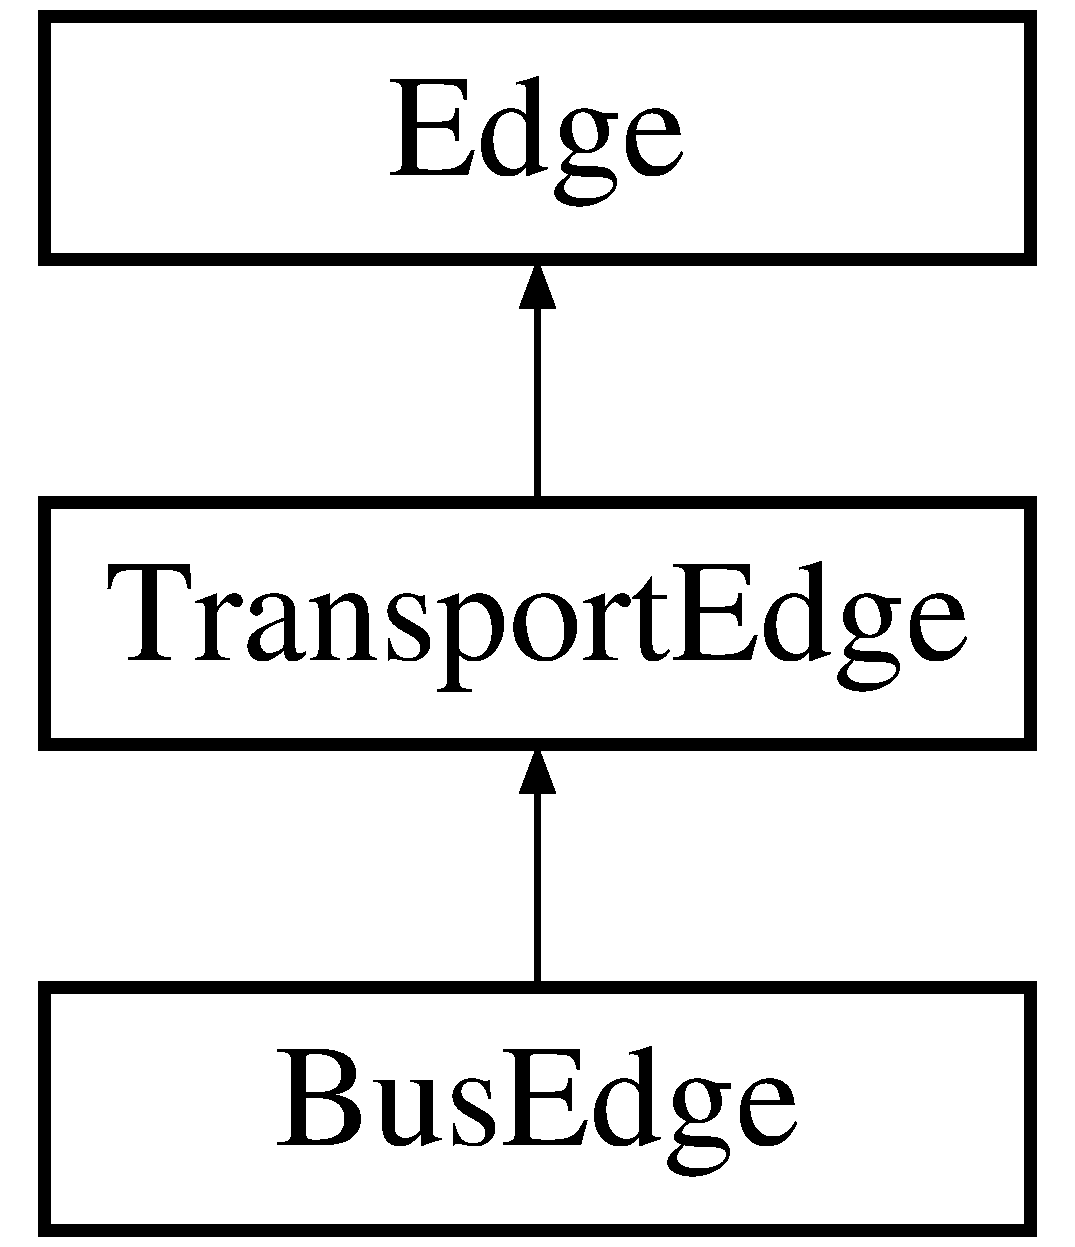
\includegraphics[height=3.000000cm]{class_bus_edge}
\end{center}
\end{figure}
\subsection*{Public Member Functions}
\begin{DoxyCompactItemize}
\item 
\hyperlink{class_bus_edge_a339f95411a13acf7c8b700af36a43f93}{Bus\+Edge} (\hyperlink{class_vertex}{Vertex} $\ast$src, \hyperlink{class_vertex}{Vertex} $\ast$dst, const vector$<$ \hyperlink{class_coordinates}{Coordinates} $>$ \&line)
\begin{DoxyCompactList}\small\item\em bus edge constructor \end{DoxyCompactList}\item 
\hypertarget{class_bus_edge_a8724578c3c10c755f3936e754c58bf57}{}void \hyperlink{class_bus_edge_a8724578c3c10c755f3936e754c58bf57}{print} () const \label{class_bus_edge_a8724578c3c10c755f3936e754c58bf57}

\begin{DoxyCompactList}\small\item\em print the busedge \end{DoxyCompactList}\item 
virtual double \hyperlink{class_bus_edge_ad89c82a7f0bf9a49610b5ef437f3dcca}{get\+Speed} () const 
\begin{DoxyCompactList}\small\item\em get the speed of a bus \end{DoxyCompactList}\item 
double \hyperlink{class_bus_edge_a186045a2fc5cf2694390552627b5f985}{get\+Weight} ()
\begin{DoxyCompactList}\small\item\em get weight of edge \end{DoxyCompactList}\item 
\hypertarget{class_bus_edge_ab8473fb0562c52e08ff70ae0b3ccf6b4}{}virtual \hyperlink{class_bus_edge_ab8473fb0562c52e08ff70ae0b3ccf6b4}{$\sim$\+Bus\+Edge} ()\label{class_bus_edge_ab8473fb0562c52e08ff70ae0b3ccf6b4}

\begin{DoxyCompactList}\small\item\em edge destructor \end{DoxyCompactList}\end{DoxyCompactItemize}
\subsection*{Additional Inherited Members}


\subsection{Detailed Description}
represents a connection between two \hyperlink{class_bus_stop}{Bus\+Stop} \textquotesingle{}s 

\subsection{Constructor \& Destructor Documentation}
\hypertarget{class_bus_edge_a339f95411a13acf7c8b700af36a43f93}{}\index{Bus\+Edge@{Bus\+Edge}!Bus\+Edge@{Bus\+Edge}}
\index{Bus\+Edge@{Bus\+Edge}!Bus\+Edge@{Bus\+Edge}}
\subsubsection[{Bus\+Edge}]{\setlength{\rightskip}{0pt plus 5cm}Bus\+Edge\+::\+Bus\+Edge (
\begin{DoxyParamCaption}
\item[{{\bf Vertex} $\ast$}]{src, }
\item[{{\bf Vertex} $\ast$}]{dst, }
\item[{const vector$<$ {\bf Coordinates} $>$ \&}]{line}
\end{DoxyParamCaption}
)}\label{class_bus_edge_a339f95411a13acf7c8b700af36a43f93}


bus edge constructor 


\begin{DoxyParams}{Parameters}
{\em src} & source vertex for edge \\
\hline
{\em dst} & source vertex for edge \\
\hline
{\em line} & set of points for the line \\
\hline
\end{DoxyParams}


\subsection{Member Function Documentation}
\hypertarget{class_bus_edge_ad89c82a7f0bf9a49610b5ef437f3dcca}{}\index{Bus\+Edge@{Bus\+Edge}!get\+Speed@{get\+Speed}}
\index{get\+Speed@{get\+Speed}!Bus\+Edge@{Bus\+Edge}}
\subsubsection[{get\+Speed}]{\setlength{\rightskip}{0pt plus 5cm}double Bus\+Edge\+::get\+Speed (
\begin{DoxyParamCaption}
{}
\end{DoxyParamCaption}
) const\hspace{0.3cm}{\ttfamily [virtual]}}\label{class_bus_edge_ad89c82a7f0bf9a49610b5ef437f3dcca}


get the speed of a bus 

\begin{DoxyReturn}{Returns}
bus speed 
\end{DoxyReturn}


Reimplemented from \hyperlink{class_transport_edge_a1e85cb198714507e2b1466b86f97b676}{Transport\+Edge}.

\hypertarget{class_bus_edge_a186045a2fc5cf2694390552627b5f985}{}\index{Bus\+Edge@{Bus\+Edge}!get\+Weight@{get\+Weight}}
\index{get\+Weight@{get\+Weight}!Bus\+Edge@{Bus\+Edge}}
\subsubsection[{get\+Weight}]{\setlength{\rightskip}{0pt plus 5cm}double Bus\+Edge\+::get\+Weight (
\begin{DoxyParamCaption}
{}
\end{DoxyParamCaption}
)\hspace{0.3cm}{\ttfamily [virtual]}}\label{class_bus_edge_a186045a2fc5cf2694390552627b5f985}


get weight of edge 

\begin{DoxyReturn}{Returns}
weight of edge 
\end{DoxyReturn}


Reimplemented from \hyperlink{class_transport_edge_ad2b8f66adec9223e97752ae1fb621c0e}{Transport\+Edge}.



The documentation for this class was generated from the following files\+:\begin{DoxyCompactItemize}
\item 
C\+:/\+Users/\+André/\+Desktop/test/transport/Bus\+Edge.\+h\item 
C\+:/\+Users/\+André/\+Desktop/test/transport/Bus\+Edge.\+cpp\end{DoxyCompactItemize}

\hypertarget{class_bus_route}{}\section{Bus\+Route Class Reference}
\label{class_bus_route}\index{Bus\+Route@{Bus\+Route}}


Represents a \hyperlink{class_bus_route}{Bus\+Route}, having a set of \hyperlink{class_bus_stop}{Bus\+Stop} \textquotesingle{}s ordered in a certain way.  




{\ttfamily \#include $<$Bus\+Route.\+h$>$}

Inheritance diagram for Bus\+Route\+:\begin{figure}[H]
\begin{center}
\leavevmode
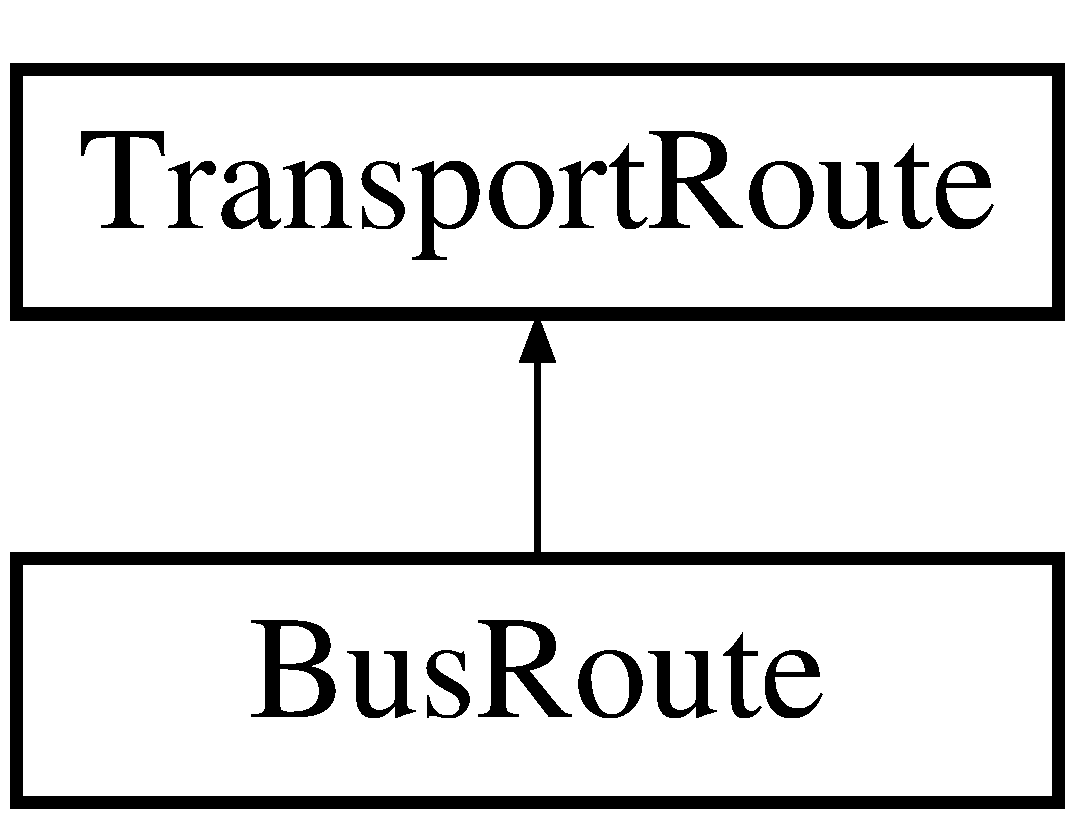
\includegraphics[height=2.000000cm]{class_bus_route}
\end{center}
\end{figure}
\subsection*{Public Member Functions}
\begin{DoxyCompactItemize}
\item 
\hyperlink{class_bus_route_a5b3f97c70fab168657fa24078bb4eecb}{Bus\+Route} (const std\+::string code, bool direction)
\begin{DoxyCompactList}\small\item\em bus route construtor \end{DoxyCompactList}\item 
double \hyperlink{class_bus_route_a6fd549a61adf27ce8a56259326fdc241}{get\+Speed} () const 
\begin{DoxyCompactList}\small\item\em get speed of buses \end{DoxyCompactList}\end{DoxyCompactItemize}
\subsection*{Static Public Attributes}
\begin{DoxyCompactItemize}
\item 
\hypertarget{class_bus_route_aca2d92a6ac67d67bf19654750ab26938}{}static const double {\bfseries speed} = 1\label{class_bus_route_aca2d92a6ac67d67bf19654750ab26938}

\end{DoxyCompactItemize}
\subsection*{Additional Inherited Members}


\subsection{Detailed Description}
Represents a \hyperlink{class_bus_route}{Bus\+Route}, having a set of \hyperlink{class_bus_stop}{Bus\+Stop} \textquotesingle{}s ordered in a certain way. 

\subsection{Constructor \& Destructor Documentation}
\hypertarget{class_bus_route_a5b3f97c70fab168657fa24078bb4eecb}{}\index{Bus\+Route@{Bus\+Route}!Bus\+Route@{Bus\+Route}}
\index{Bus\+Route@{Bus\+Route}!Bus\+Route@{Bus\+Route}}
\subsubsection[{Bus\+Route}]{\setlength{\rightskip}{0pt plus 5cm}Bus\+Route\+::\+Bus\+Route (
\begin{DoxyParamCaption}
\item[{const std\+::string}]{code, }
\item[{bool}]{direction}
\end{DoxyParamCaption}
)}\label{class_bus_route_a5b3f97c70fab168657fa24078bb4eecb}


bus route construtor 


\begin{DoxyParams}{Parameters}
{\em code} & code of busroute \\
\hline
{\em direction} & direction of route \\
\hline
\end{DoxyParams}


\subsection{Member Function Documentation}
\hypertarget{class_bus_route_a6fd549a61adf27ce8a56259326fdc241}{}\index{Bus\+Route@{Bus\+Route}!get\+Speed@{get\+Speed}}
\index{get\+Speed@{get\+Speed}!Bus\+Route@{Bus\+Route}}
\subsubsection[{get\+Speed}]{\setlength{\rightskip}{0pt plus 5cm}double Bus\+Route\+::get\+Speed (
\begin{DoxyParamCaption}
{}
\end{DoxyParamCaption}
) const\hspace{0.3cm}{\ttfamily [virtual]}}\label{class_bus_route_a6fd549a61adf27ce8a56259326fdc241}


get speed of buses 

\begin{DoxyReturn}{Returns}
buss speed 
\end{DoxyReturn}


Implements \hyperlink{class_transport_route_a76a8834e9595e973f61f3376ff3d9d34}{Transport\+Route}.



The documentation for this class was generated from the following files\+:\begin{DoxyCompactItemize}
\item 
C\+:/\+Users/\+André/\+Desktop/test/transport/Bus\+Route.\+h\item 
C\+:/\+Users/\+André/\+Desktop/test/transport/Bus\+Route.\+cpp\end{DoxyCompactItemize}

\hypertarget{class_bus_stop}{}\section{Bus\+Stop Class Reference}
\label{class_bus_stop}\index{Bus\+Stop@{Bus\+Stop}}


Represents a bus stop.  




{\ttfamily \#include $<$Bus\+Stop.\+h$>$}

Inheritance diagram for Bus\+Stop\+:\begin{figure}[H]
\begin{center}
\leavevmode
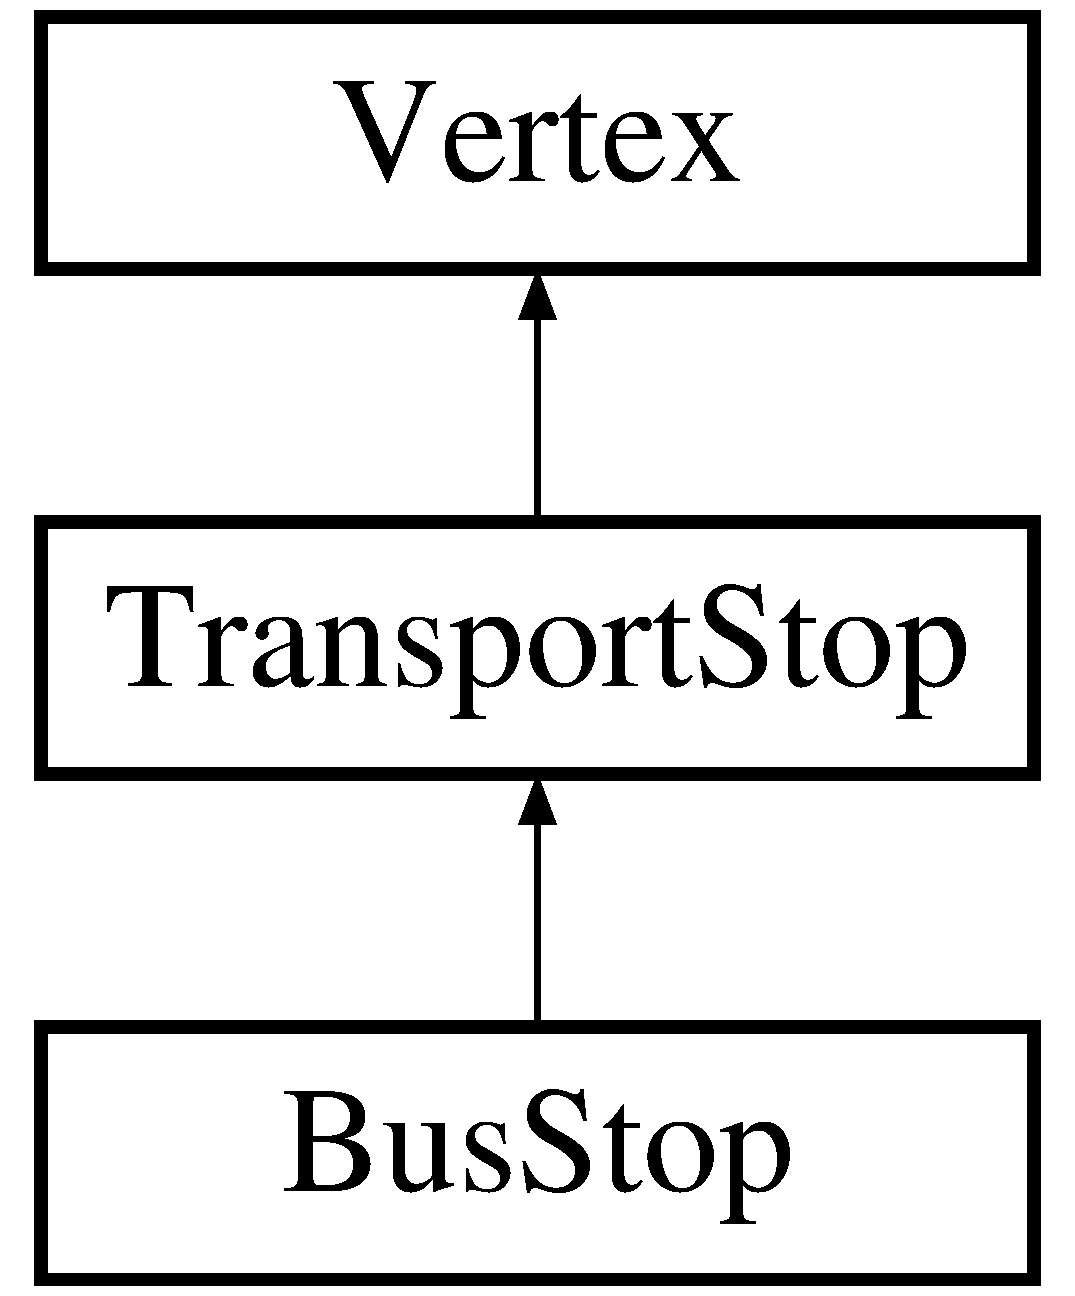
\includegraphics[height=3.000000cm]{class_bus_stop}
\end{center}
\end{figure}
\subsection*{Public Member Functions}
\begin{DoxyCompactItemize}
\item 
\hyperlink{class_bus_stop_ab48e6ec461fef340bb522e3569db716d}{Bus\+Stop} (const std\+::string \&code, const std\+::string \&name, const \hyperlink{class_coordinates}{Coordinates} \&coords, const std\+::string \&route\+\_\+name)
\begin{DoxyCompactList}\small\item\em bus stop construtor \end{DoxyCompactList}\item 
const string \& \hyperlink{class_bus_stop_a894b79e4e5582c9c89c3abc103c3a545}{get\+Code} () const 
\begin{DoxyCompactList}\small\item\em bus stop\textquotesingle{}s code \end{DoxyCompactList}\item 
\hypertarget{class_bus_stop_a8fa0c0a7f5252cd74a2e3337ef4e27e9}{}void \hyperlink{class_bus_stop_a8fa0c0a7f5252cd74a2e3337ef4e27e9}{print} () const \label{class_bus_stop_a8fa0c0a7f5252cd74a2e3337ef4e27e9}

\begin{DoxyCompactList}\small\item\em print the bus stop \end{DoxyCompactList}\item 
virtual std\+::string \hyperlink{class_bus_stop_a508c7cf008dcb6072ce4a5179cefd42d}{get\+Name\+And\+Type} () const 
\begin{DoxyCompactList}\small\item\em get a string containing the name of the stop and its type \end{DoxyCompactList}\end{DoxyCompactItemize}
\subsection*{Additional Inherited Members}


\subsection{Detailed Description}
Represents a bus stop. 

\subsection{Constructor \& Destructor Documentation}
\hypertarget{class_bus_stop_ab48e6ec461fef340bb522e3569db716d}{}\index{Bus\+Stop@{Bus\+Stop}!Bus\+Stop@{Bus\+Stop}}
\index{Bus\+Stop@{Bus\+Stop}!Bus\+Stop@{Bus\+Stop}}
\subsubsection[{Bus\+Stop}]{\setlength{\rightskip}{0pt plus 5cm}Bus\+Stop\+::\+Bus\+Stop (
\begin{DoxyParamCaption}
\item[{const std\+::string \&}]{code, }
\item[{const std\+::string \&}]{name, }
\item[{const {\bf Coordinates} \&}]{coords, }
\item[{const std\+::string \&}]{route\+\_\+name}
\end{DoxyParamCaption}
)}\label{class_bus_stop_ab48e6ec461fef340bb522e3569db716d}


bus stop construtor 


\begin{DoxyParams}{Parameters}
{\em code} & code of bus stop \\
\hline
{\em name} & name of bus stop \\
\hline
{\em coords} & coordinates of bus stop to create \\
\hline
{\em route\+\_\+name} & name of the stop\textquotesingle{}s route \\
\hline
\end{DoxyParams}


\subsection{Member Function Documentation}
\hypertarget{class_bus_stop_a894b79e4e5582c9c89c3abc103c3a545}{}\index{Bus\+Stop@{Bus\+Stop}!get\+Code@{get\+Code}}
\index{get\+Code@{get\+Code}!Bus\+Stop@{Bus\+Stop}}
\subsubsection[{get\+Code}]{\setlength{\rightskip}{0pt plus 5cm}const string\& Bus\+Stop\+::get\+Code (
\begin{DoxyParamCaption}
{}
\end{DoxyParamCaption}
) const\hspace{0.3cm}{\ttfamily [inline]}}\label{class_bus_stop_a894b79e4e5582c9c89c3abc103c3a545}


bus stop\textquotesingle{}s code 

\begin{DoxyReturn}{Returns}
code of bus stop 
\end{DoxyReturn}
\hypertarget{class_bus_stop_a508c7cf008dcb6072ce4a5179cefd42d}{}\index{Bus\+Stop@{Bus\+Stop}!get\+Name\+And\+Type@{get\+Name\+And\+Type}}
\index{get\+Name\+And\+Type@{get\+Name\+And\+Type}!Bus\+Stop@{Bus\+Stop}}
\subsubsection[{get\+Name\+And\+Type}]{\setlength{\rightskip}{0pt plus 5cm}virtual std\+::string Bus\+Stop\+::get\+Name\+And\+Type (
\begin{DoxyParamCaption}
{}
\end{DoxyParamCaption}
) const\hspace{0.3cm}{\ttfamily [inline]}, {\ttfamily [virtual]}}\label{class_bus_stop_a508c7cf008dcb6072ce4a5179cefd42d}


get a string containing the name of the stop and its type 

\begin{DoxyReturn}{Returns}
string containing the information 
\end{DoxyReturn}


Reimplemented from \hyperlink{class_transport_stop_a245cff19d0ef473d56b93036042478ef}{Transport\+Stop}.



The documentation for this class was generated from the following files\+:\begin{DoxyCompactItemize}
\item 
C\+:/\+Users/\+André/\+Desktop/test/transport/Bus\+Stop.\+h\item 
C\+:/\+Users/\+André/\+Desktop/test/transport/Bus\+Stop.\+cpp\end{DoxyCompactItemize}

\hypertarget{class_camera}{}\section{Camera Class Reference}
\label{class_camera}\index{Camera@{Camera}}


Implements a camera, able to zoom and drag in the graphical interface.  




{\ttfamily \#include $<$Camera.\+h$>$}

\subsection*{Public Member Functions}
\begin{DoxyCompactItemize}
\item 
\hypertarget{class_camera_a216588630410cfa52c6adaf374e240da}{}{\bfseries Camera} (double x0, double y0, double x1, double y1, double limit)\label{class_camera_a216588630410cfa52c6adaf374e240da}

\item 
\hypertarget{class_camera_a7133510d8b81dd969f44d21f07323246}{}void {\bfseries move\+Abs} (double x, double y)\label{class_camera_a7133510d8b81dd969f44d21f07323246}

\item 
\hypertarget{class_camera_aaa843df2a2989b898215726effa15cac}{}void {\bfseries move\+Partial\+Abs\+Centered} (double x, double y, int h\+\_\+res, int v\+\_\+res, double extent=1.\+0)\label{class_camera_aaa843df2a2989b898215726effa15cac}

\item 
\hypertarget{class_camera_a7dd0597323b13c42fee51a6dbb9ca935}{}void {\bfseries move\+Rel} (double x, double y)\label{class_camera_a7dd0597323b13c42fee51a6dbb9ca935}

\item 
\hypertarget{class_camera_a7ae9de71e0fa685debfc94db003b9d8b}{}void {\bfseries move\+Rel\+Scaled} (double x, double y, int h\+\_\+res, int v\+\_\+res)\label{class_camera_a7ae9de71e0fa685debfc94db003b9d8b}

\item 
\hypertarget{class_camera_a0e4d6f609f47758434f7d699226a5450}{}void {\bfseries move\+Rel\+Screen} (double x, double y, int h\+\_\+res, int v\+\_\+res)\label{class_camera_a0e4d6f609f47758434f7d699226a5450}

\item 
\hypertarget{class_camera_a389acf34b48d163f610f7fda36f715da}{}bool {\bfseries mul\+Scale} (double factorx, double factory)\label{class_camera_a389acf34b48d163f610f7fda36f715da}

\item 
\hypertarget{class_camera_a6da74cb911cf06f04bfaf38418fc77a9}{}bool {\bfseries uncentered\+Mul\+Scale} (double factorx, double factory, double x, double y, int h\+\_\+res, int v\+\_\+res)\label{class_camera_a6da74cb911cf06f04bfaf38418fc77a9}

\item 
\hypertarget{class_camera_ae21745d73e59d4a4a4e27a12a9cf91cb}{}void {\bfseries add\+Scale} (double addx, double addy)\label{class_camera_ae21745d73e59d4a4a4e27a12a9cf91cb}

\item 
\hypertarget{class_camera_a1f42a416c08d8328a4f6723bf7feafd9}{}void {\bfseries add\+Scale\+Uniform} (double add, bool on\+Width=true)\label{class_camera_a1f42a416c08d8328a4f6723bf7feafd9}

\item 
\hypertarget{class_camera_a379f195daa407ca0a9e76f47dae01ea2}{}double {\bfseries get\+X} () const \label{class_camera_a379f195daa407ca0a9e76f47dae01ea2}

\item 
\hypertarget{class_camera_a7f40c406bf769ac6fd6f3898f661f9b6}{}double {\bfseries get\+Y} () const \label{class_camera_a7f40c406bf769ac6fd6f3898f661f9b6}

\item 
\hypertarget{class_camera_abb31feca14c773a36d08d44d19f957ba}{}double {\bfseries get\+Final\+X} () const \label{class_camera_abb31feca14c773a36d08d44d19f957ba}

\item 
\hypertarget{class_camera_a842f8054c5348f32df5df432d88e9560}{}double {\bfseries get\+Final\+Y} () const \label{class_camera_a842f8054c5348f32df5df432d88e9560}

\item 
\hypertarget{class_camera_aee1e6f2957c75bb15068cd94d5cf08c4}{}double {\bfseries get\+Width} () const \label{class_camera_aee1e6f2957c75bb15068cd94d5cf08c4}

\item 
\hypertarget{class_camera_a8ce5a105319bd85379b669b004b1b3c9}{}double {\bfseries get\+Height} () const \label{class_camera_a8ce5a105319bd85379b669b004b1b3c9}

\item 
\hypertarget{class_camera_aeb960f4f7775bbc7abb34b8d7f667866}{}double {\bfseries get\+Render\+X} (int h\+\_\+res, double world\+X) const \label{class_camera_aeb960f4f7775bbc7abb34b8d7f667866}

\item 
\hypertarget{class_camera_a6af6702c0ef40d7cdb1d396a673af290}{}double {\bfseries get\+Render\+Y} (int v\+\_\+res, double world\+Y) const \label{class_camera_a6af6702c0ef40d7cdb1d396a673af290}

\item 
\hypertarget{class_camera_a509ea65044ffbd771f2ca3aa72040ef5}{}double {\bfseries get\+World\+X} (int h\+\_\+res, double render\+X) const \label{class_camera_a509ea65044ffbd771f2ca3aa72040ef5}

\item 
\hypertarget{class_camera_acfe0129236a227ab6203f83421552c83}{}double {\bfseries get\+World\+Y} (int v\+\_\+res, double render\+Y) const \label{class_camera_acfe0129236a227ab6203f83421552c83}

\item 
\hypertarget{class_camera_acca75da7b31a6d894673250ece0eb9c1}{}double {\bfseries get\+Zoom\+Scale\+X} () const \label{class_camera_acca75da7b31a6d894673250ece0eb9c1}

\item 
\hypertarget{class_camera_ae87bd07393cdd700fcc87d698d1011c2}{}double {\bfseries get\+Zoom\+Scale\+Y} () const \label{class_camera_ae87bd07393cdd700fcc87d698d1011c2}

\end{DoxyCompactItemize}


\subsection{Detailed Description}
Implements a camera, able to zoom and drag in the graphical interface. 

The documentation for this class was generated from the following files\+:\begin{DoxyCompactItemize}
\item 
C\+:/\+Users/\+André/\+Desktop/test/gui/Camera.\+h\item 
C\+:/\+Users/\+André/\+Desktop/test/gui/Camera.\+cpp\end{DoxyCompactItemize}

\hypertarget{class_coordinates}{}\section{Coordinates Class Reference}
\label{class_coordinates}\index{Coordinates@{Coordinates}}


Interface to store latitude and longitude of points.  




{\ttfamily \#include $<$Coordinates.\+h$>$}

\subsection*{Public Member Functions}
\begin{DoxyCompactItemize}
\item 
\hyperlink{class_coordinates_a008a2acb31c4606eac1969bc5f1892f0}{Coordinates} (double latitude, double longitude)
\begin{DoxyCompactList}\small\item\em coordinate constructor \end{DoxyCompactList}\item 
double \hyperlink{class_coordinates_aad64e70c40d1f25458b122559e289c7d}{get\+Latitude} () const 
\begin{DoxyCompactList}\small\item\em get latitude of coordinate \end{DoxyCompactList}\item 
double \hyperlink{class_coordinates_a865746116df79ade68631f5bb695c591}{get\+Longitude} () const 
\begin{DoxyCompactList}\small\item\em get longitude of coordinate \end{DoxyCompactList}\item 
double \hyperlink{class_coordinates_ae5a68f6d9304775a18af48bc3d0fef52}{calc\+Dist} (const \hyperlink{class_coordinates}{Coordinates} \&coordinates) const 
\begin{DoxyCompactList}\small\item\em bus stop construtor \end{DoxyCompactList}\item 
double \hyperlink{class_coordinates_ac0ab9ce22061bba4e6db2c4c27da398c}{calc\+Direct\+Dist\+Square} (const \hyperlink{class_coordinates}{Coordinates} \&coordinates) const 
\begin{DoxyCompactList}\small\item\em bus stop construtor \end{DoxyCompactList}\end{DoxyCompactItemize}


\subsection{Detailed Description}
Interface to store latitude and longitude of points. 

\subsection{Constructor \& Destructor Documentation}
\hypertarget{class_coordinates_a008a2acb31c4606eac1969bc5f1892f0}{}\index{Coordinates@{Coordinates}!Coordinates@{Coordinates}}
\index{Coordinates@{Coordinates}!Coordinates@{Coordinates}}
\subsubsection[{Coordinates}]{\setlength{\rightskip}{0pt plus 5cm}Coordinates\+::\+Coordinates (
\begin{DoxyParamCaption}
\item[{double}]{latitude, }
\item[{double}]{longitude}
\end{DoxyParamCaption}
)}\label{class_coordinates_a008a2acb31c4606eac1969bc5f1892f0}


coordinate constructor 


\begin{DoxyParams}{Parameters}
{\em latitude} & latitude of coordinate \\
\hline
{\em longitude} & longitude of coordinate \\
\hline
\end{DoxyParams}


\subsection{Member Function Documentation}
\hypertarget{class_coordinates_ac0ab9ce22061bba4e6db2c4c27da398c}{}\index{Coordinates@{Coordinates}!calc\+Direct\+Dist\+Square@{calc\+Direct\+Dist\+Square}}
\index{calc\+Direct\+Dist\+Square@{calc\+Direct\+Dist\+Square}!Coordinates@{Coordinates}}
\subsubsection[{calc\+Direct\+Dist\+Square}]{\setlength{\rightskip}{0pt plus 5cm}double Coordinates\+::calc\+Direct\+Dist\+Square (
\begin{DoxyParamCaption}
\item[{const {\bf Coordinates} \&}]{coordinates}
\end{DoxyParamCaption}
) const}\label{class_coordinates_ac0ab9ce22061bba4e6db2c4c27da398c}


bus stop construtor 


\begin{DoxyParams}{Parameters}
{\em code} & code of bus stop \\
\hline
{\em name} & name of bus stop \\
\hline
{\em coords} & coordinates of bus stop to create \\
\hline
\end{DoxyParams}
\hypertarget{class_coordinates_ae5a68f6d9304775a18af48bc3d0fef52}{}\index{Coordinates@{Coordinates}!calc\+Dist@{calc\+Dist}}
\index{calc\+Dist@{calc\+Dist}!Coordinates@{Coordinates}}
\subsubsection[{calc\+Dist}]{\setlength{\rightskip}{0pt plus 5cm}double Coordinates\+::calc\+Dist (
\begin{DoxyParamCaption}
\item[{const {\bf Coordinates} \&}]{coordinates}
\end{DoxyParamCaption}
) const}\label{class_coordinates_ae5a68f6d9304775a18af48bc3d0fef52}


bus stop construtor 


\begin{DoxyParams}{Parameters}
{\em code} & code of bus stop \\
\hline
{\em name} & name of bus stop \\
\hline
{\em coords} & coordinates of bus stop to create \\
\hline
\end{DoxyParams}
\hypertarget{class_coordinates_aad64e70c40d1f25458b122559e289c7d}{}\index{Coordinates@{Coordinates}!get\+Latitude@{get\+Latitude}}
\index{get\+Latitude@{get\+Latitude}!Coordinates@{Coordinates}}
\subsubsection[{get\+Latitude}]{\setlength{\rightskip}{0pt plus 5cm}double Coordinates\+::get\+Latitude (
\begin{DoxyParamCaption}
{}
\end{DoxyParamCaption}
) const}\label{class_coordinates_aad64e70c40d1f25458b122559e289c7d}


get latitude of coordinate 

\begin{DoxyReturn}{Returns}
latitude of coordinate 
\end{DoxyReturn}
\hypertarget{class_coordinates_a865746116df79ade68631f5bb695c591}{}\index{Coordinates@{Coordinates}!get\+Longitude@{get\+Longitude}}
\index{get\+Longitude@{get\+Longitude}!Coordinates@{Coordinates}}
\subsubsection[{get\+Longitude}]{\setlength{\rightskip}{0pt plus 5cm}double Coordinates\+::get\+Longitude (
\begin{DoxyParamCaption}
{}
\end{DoxyParamCaption}
) const}\label{class_coordinates_a865746116df79ade68631f5bb695c591}


get longitude of coordinate 

\begin{DoxyReturn}{Returns}
longitude of coordinate 
\end{DoxyReturn}


The documentation for this class was generated from the following files\+:\begin{DoxyCompactItemize}
\item 
C\+:/\+Users/\+André/\+Desktop/test/transport/Coordinates.\+h\item 
C\+:/\+Users/\+André/\+Desktop/test/transport/Coordinates.\+cpp\end{DoxyCompactItemize}

\hypertarget{struct_vertex_1_1_dijs_comp}{}\section{Vertex\+:\+:Dijs\+Comp Struct Reference}
\label{struct_vertex_1_1_dijs_comp}\index{Vertex\+::\+Dijs\+Comp@{Vertex\+::\+Dijs\+Comp}}


comparison struct for ordering of vertex pointers for use in Dijkstra\textquotesingle{}s algorithm  




{\ttfamily \#include $<$Vertex.\+h$>$}

\subsection*{Public Member Functions}
\begin{DoxyCompactItemize}
\item 
bool \hyperlink{struct_vertex_1_1_dijs_comp_a4d0ace3727b7cf44dfbbaea180ab6a29}{operator()} (\hyperlink{class_vertex}{Vertex} $\ast$v1, \hyperlink{class_vertex}{Vertex} $\ast$v2) const 
\begin{DoxyCompactList}\small\item\em comparison operator \end{DoxyCompactList}\end{DoxyCompactItemize}


\subsection{Detailed Description}
comparison struct for ordering of vertex pointers for use in Dijkstra\textquotesingle{}s algorithm 

\subsection{Member Function Documentation}
\hypertarget{struct_vertex_1_1_dijs_comp_a4d0ace3727b7cf44dfbbaea180ab6a29}{}\index{Vertex\+::\+Dijs\+Comp@{Vertex\+::\+Dijs\+Comp}!operator()@{operator()}}
\index{operator()@{operator()}!Vertex\+::\+Dijs\+Comp@{Vertex\+::\+Dijs\+Comp}}
\subsubsection[{operator()}]{\setlength{\rightskip}{0pt plus 5cm}bool Vertex\+::\+Dijs\+Comp\+::operator() (
\begin{DoxyParamCaption}
\item[{{\bf Vertex} $\ast$}]{v1, }
\item[{{\bf Vertex} $\ast$}]{v2}
\end{DoxyParamCaption}
) const\hspace{0.3cm}{\ttfamily [inline]}}\label{struct_vertex_1_1_dijs_comp_a4d0ace3727b7cf44dfbbaea180ab6a29}


comparison operator 


\begin{DoxyParams}{Parameters}
{\em v1} & first vertex to compare \\
\hline
{\em v2} & second vertex to compare \\
\hline
\end{DoxyParams}


The documentation for this struct was generated from the following file\+:\begin{DoxyCompactItemize}
\item 
C\+:/\+Users/\+André/\+Desktop/test/graph/Vertex.\+h\end{DoxyCompactItemize}

\hypertarget{class_edge}{}\section{Edge Class Reference}
\label{class_edge}\index{Edge@{Edge}}


Generic \hyperlink{class_edge}{Edge} interface.  




{\ttfamily \#include $<$Edge.\+h$>$}

Inheritance diagram for Edge\+:\begin{figure}[H]
\begin{center}
\leavevmode
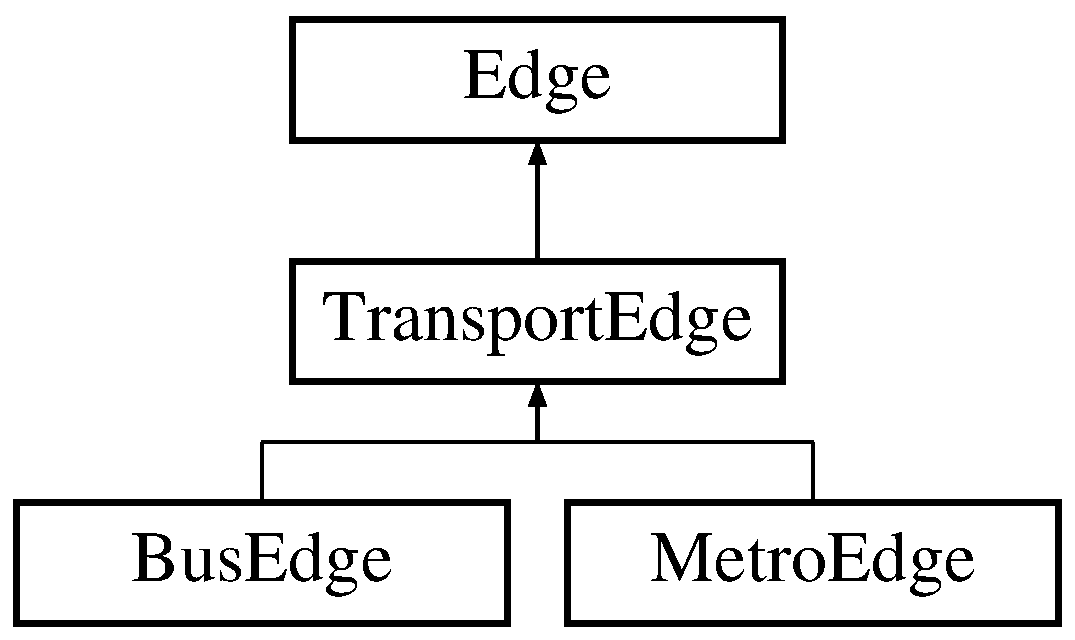
\includegraphics[height=3.000000cm]{class_edge}
\end{center}
\end{figure}
\subsection*{Public Member Functions}
\begin{DoxyCompactItemize}
\item 
\hyperlink{class_edge_a175c30ff76609608a96c498c13ef55b0}{Edge} (\hyperlink{class_vertex}{Vertex} $\ast$src, \hyperlink{class_vertex}{Vertex} $\ast$dst, double stored\+Weight=0)
\begin{DoxyCompactList}\small\item\em edge construtor \end{DoxyCompactList}\item 
virtual double \hyperlink{class_edge_a3a776c1ccafacdbdb10fdedd9cb329af}{get\+Weight} ()
\begin{DoxyCompactList}\small\item\em get the weight of this edge \end{DoxyCompactList}\item 
virtual void \hyperlink{class_edge_af7851a1bcd26d69b03010c85ae26be4d}{set\+Stored\+Weight} (double stored\+Weight)
\begin{DoxyCompactList}\small\item\em store a weight value in edge \end{DoxyCompactList}\item 
virtual \hyperlink{class_vertex}{Vertex} $\ast$ \hyperlink{class_edge_ac8602ef0c7762e086a719e5c300e80b8}{get\+Dst} () const 
\begin{DoxyCompactList}\small\item\em get the destination of this edge \end{DoxyCompactList}\item 
virtual void \hyperlink{class_edge_a43d8bf7d905ff0a4df84b2634e8e9860}{set\+Dst} (\hyperlink{class_vertex}{Vertex} $\ast$dst)
\begin{DoxyCompactList}\small\item\em set the destination of this edge \end{DoxyCompactList}\item 
virtual \hyperlink{class_vertex}{Vertex} $\ast$ \hyperlink{class_edge_a9942c08298b9abcdd39918c1e723ab6a}{get\+Src} () const 
\begin{DoxyCompactList}\small\item\em get the source of this edge \end{DoxyCompactList}\item 
virtual void \hyperlink{class_edge_af48131d832408a09b41ce0b39361c2ab}{set\+Src} (\hyperlink{class_vertex}{Vertex} $\ast$src)
\begin{DoxyCompactList}\small\item\em set the source of this edge \end{DoxyCompactList}\item 
\hypertarget{class_edge_afe6e80534a1f9805d2e8730d0d4d5cc7}{}virtual void \hyperlink{class_edge_afe6e80534a1f9805d2e8730d0d4d5cc7}{store\+Weight} ()\label{class_edge_afe6e80534a1f9805d2e8730d0d4d5cc7}

\begin{DoxyCompactList}\small\item\em store weight in edge \end{DoxyCompactList}\item 
virtual double \hyperlink{class_edge_a1ea100fde60c88afd5eb6f5b7829b796}{get\+Stored\+Weight} () const 
\begin{DoxyCompactList}\small\item\em retrived weight stored in edge \end{DoxyCompactList}\item 
virtual \hyperlink{class_s_d_l_r_g_b}{S\+D\+L\+R\+G\+B} \hyperlink{class_edge_a16081643290e304fd50a39144a716e2d}{get\+Color} ()
\begin{DoxyCompactList}\small\item\em get the vertex\textquotesingle{}s color \end{DoxyCompactList}\item 
\hypertarget{class_edge_a2f37b72f044427961d6730943daf10e0}{}virtual \hyperlink{class_edge_a2f37b72f044427961d6730943daf10e0}{$\sim$\+Edge} ()\label{class_edge_a2f37b72f044427961d6730943daf10e0}

\begin{DoxyCompactList}\small\item\em edge destructor \end{DoxyCompactList}\end{DoxyCompactItemize}
\subsection*{Protected Attributes}
\begin{DoxyCompactItemize}
\item 
\hypertarget{class_edge_a94f44a5a7b1110641414bc2e00a4ba2f}{}double {\bfseries stored\+Weight}\label{class_edge_a94f44a5a7b1110641414bc2e00a4ba2f}

\end{DoxyCompactItemize}


\subsection{Detailed Description}
Generic \hyperlink{class_edge}{Edge} interface. 

\subsection{Constructor \& Destructor Documentation}
\hypertarget{class_edge_a175c30ff76609608a96c498c13ef55b0}{}\index{Edge@{Edge}!Edge@{Edge}}
\index{Edge@{Edge}!Edge@{Edge}}
\subsubsection[{Edge}]{\setlength{\rightskip}{0pt plus 5cm}Edge\+::\+Edge (
\begin{DoxyParamCaption}
\item[{{\bf Vertex} $\ast$}]{src, }
\item[{{\bf Vertex} $\ast$}]{dst, }
\item[{double}]{stored\+Weight = {\ttfamily 0}}
\end{DoxyParamCaption}
)}\label{class_edge_a175c30ff76609608a96c498c13ef55b0}


edge construtor 


\begin{DoxyParams}{Parameters}
{\em src} & source vertex for edge \\
\hline
{\em dst} & source vertex for edge \\
\hline
{\em stored\+Weight} & source vertex for edge \\
\hline
\end{DoxyParams}


\subsection{Member Function Documentation}
\hypertarget{class_edge_a16081643290e304fd50a39144a716e2d}{}\index{Edge@{Edge}!get\+Color@{get\+Color}}
\index{get\+Color@{get\+Color}!Edge@{Edge}}
\subsubsection[{get\+Color}]{\setlength{\rightskip}{0pt plus 5cm}{\bf S\+D\+L\+R\+G\+B} Edge\+::get\+Color (
\begin{DoxyParamCaption}
{}
\end{DoxyParamCaption}
)\hspace{0.3cm}{\ttfamily [virtual]}}\label{class_edge_a16081643290e304fd50a39144a716e2d}


get the vertex\textquotesingle{}s color 

\begin{DoxyReturn}{Returns}
color of vertex 
\end{DoxyReturn}
\hypertarget{class_edge_ac8602ef0c7762e086a719e5c300e80b8}{}\index{Edge@{Edge}!get\+Dst@{get\+Dst}}
\index{get\+Dst@{get\+Dst}!Edge@{Edge}}
\subsubsection[{get\+Dst}]{\setlength{\rightskip}{0pt plus 5cm}{\bf Vertex} $\ast$ Edge\+::get\+Dst (
\begin{DoxyParamCaption}
{}
\end{DoxyParamCaption}
) const\hspace{0.3cm}{\ttfamily [virtual]}}\label{class_edge_ac8602ef0c7762e086a719e5c300e80b8}


get the destination of this edge 

\begin{DoxyReturn}{Returns}
destination 
\end{DoxyReturn}
\hypertarget{class_edge_a9942c08298b9abcdd39918c1e723ab6a}{}\index{Edge@{Edge}!get\+Src@{get\+Src}}
\index{get\+Src@{get\+Src}!Edge@{Edge}}
\subsubsection[{get\+Src}]{\setlength{\rightskip}{0pt plus 5cm}{\bf Vertex} $\ast$ Edge\+::get\+Src (
\begin{DoxyParamCaption}
{}
\end{DoxyParamCaption}
) const\hspace{0.3cm}{\ttfamily [virtual]}}\label{class_edge_a9942c08298b9abcdd39918c1e723ab6a}


get the source of this edge 

\begin{DoxyReturn}{Returns}
source 
\end{DoxyReturn}
\hypertarget{class_edge_a1ea100fde60c88afd5eb6f5b7829b796}{}\index{Edge@{Edge}!get\+Stored\+Weight@{get\+Stored\+Weight}}
\index{get\+Stored\+Weight@{get\+Stored\+Weight}!Edge@{Edge}}
\subsubsection[{get\+Stored\+Weight}]{\setlength{\rightskip}{0pt plus 5cm}double Edge\+::get\+Stored\+Weight (
\begin{DoxyParamCaption}
{}
\end{DoxyParamCaption}
) const\hspace{0.3cm}{\ttfamily [virtual]}}\label{class_edge_a1ea100fde60c88afd5eb6f5b7829b796}


retrived weight stored in edge 

\begin{DoxyReturn}{Returns}
stored value 
\end{DoxyReturn}
\hypertarget{class_edge_a3a776c1ccafacdbdb10fdedd9cb329af}{}\index{Edge@{Edge}!get\+Weight@{get\+Weight}}
\index{get\+Weight@{get\+Weight}!Edge@{Edge}}
\subsubsection[{get\+Weight}]{\setlength{\rightskip}{0pt plus 5cm}double Edge\+::get\+Weight (
\begin{DoxyParamCaption}
{}
\end{DoxyParamCaption}
)\hspace{0.3cm}{\ttfamily [virtual]}}\label{class_edge_a3a776c1ccafacdbdb10fdedd9cb329af}


get the weight of this edge 

\begin{DoxyReturn}{Returns}
weight of edge 
\end{DoxyReturn}


Reimplemented in \hyperlink{class_transport_edge_ad2b8f66adec9223e97752ae1fb621c0e}{Transport\+Edge}, \hyperlink{class_bus_edge_a186045a2fc5cf2694390552627b5f985}{Bus\+Edge}, and \hyperlink{class_metro_edge_abe40bacd0e3d7e72fcdf7d0e38b2b311}{Metro\+Edge}.

\hypertarget{class_edge_a43d8bf7d905ff0a4df84b2634e8e9860}{}\index{Edge@{Edge}!set\+Dst@{set\+Dst}}
\index{set\+Dst@{set\+Dst}!Edge@{Edge}}
\subsubsection[{set\+Dst}]{\setlength{\rightskip}{0pt plus 5cm}void Edge\+::set\+Dst (
\begin{DoxyParamCaption}
\item[{{\bf Vertex} $\ast$}]{dst}
\end{DoxyParamCaption}
)\hspace{0.3cm}{\ttfamily [virtual]}}\label{class_edge_a43d8bf7d905ff0a4df84b2634e8e9860}


set the destination of this edge 


\begin{DoxyParams}{Parameters}
{\em dst} & new destination \\
\hline
\end{DoxyParams}
\hypertarget{class_edge_af48131d832408a09b41ce0b39361c2ab}{}\index{Edge@{Edge}!set\+Src@{set\+Src}}
\index{set\+Src@{set\+Src}!Edge@{Edge}}
\subsubsection[{set\+Src}]{\setlength{\rightskip}{0pt plus 5cm}void Edge\+::set\+Src (
\begin{DoxyParamCaption}
\item[{{\bf Vertex} $\ast$}]{src}
\end{DoxyParamCaption}
)\hspace{0.3cm}{\ttfamily [virtual]}}\label{class_edge_af48131d832408a09b41ce0b39361c2ab}


set the source of this edge 


\begin{DoxyParams}{Parameters}
{\em src} & new source \\
\hline
\end{DoxyParams}
\hypertarget{class_edge_af7851a1bcd26d69b03010c85ae26be4d}{}\index{Edge@{Edge}!set\+Stored\+Weight@{set\+Stored\+Weight}}
\index{set\+Stored\+Weight@{set\+Stored\+Weight}!Edge@{Edge}}
\subsubsection[{set\+Stored\+Weight}]{\setlength{\rightskip}{0pt plus 5cm}void Edge\+::set\+Stored\+Weight (
\begin{DoxyParamCaption}
\item[{double}]{stored\+Weight}
\end{DoxyParamCaption}
)\hspace{0.3cm}{\ttfamily [virtual]}}\label{class_edge_af7851a1bcd26d69b03010c85ae26be4d}


store a weight value in edge 


\begin{DoxyParams}{Parameters}
{\em value} & to store \\
\hline
\end{DoxyParams}


The documentation for this class was generated from the following files\+:\begin{DoxyCompactItemize}
\item 
C\+:/\+Users/\+André/\+Desktop/test/graph/Edge.\+h\item 
C\+:/\+Users/\+André/\+Desktop/test/graph/Edge.\+cpp\end{DoxyCompactItemize}

\hypertarget{class_graph}{}\section{Graph Class Reference}
\label{class_graph}\index{Graph@{Graph}}


Generic \hyperlink{class_graph}{Graph} interface.  




{\ttfamily \#include $<$Graph.\+h$>$}

\subsection*{Public Member Functions}
\begin{DoxyCompactItemize}
\item 
\hypertarget{class_graph_ae4c72b8ac4d693c49800a4c7e273654f}{}\hyperlink{class_graph_ae4c72b8ac4d693c49800a4c7e273654f}{Graph} ()\label{class_graph_ae4c72b8ac4d693c49800a4c7e273654f}

\begin{DoxyCompactList}\small\item\em graph constructor \end{DoxyCompactList}\item 
vector$<$ \hyperlink{class_vertex}{Vertex} $\ast$ $>$ \hyperlink{class_graph_a4cca9b48f61d44104aa2ebc959a8728c}{get\+Vertex\+Set} () const 
\begin{DoxyCompactList}\small\item\em get the list of vertices in the graph \end{DoxyCompactList}\item 
void \hyperlink{class_graph_aa95e129c42fe7150ee07d13377547324}{add\+Vertex} (\hyperlink{class_vertex}{Vertex} $\ast$v)
\begin{DoxyCompactList}\small\item\em add vertex to graph, setting its index appropriately \end{DoxyCompactList}\item 
unsigned int \hyperlink{class_graph_a89fc060f50dc936026dea4c334dd86b1}{get\+Num\+Edges} () const 
\begin{DoxyCompactList}\small\item\em count the total number of edges in graph \end{DoxyCompactList}\item 
\hypertarget{class_graph_a0d0be9182f1ff998b46122873a7d6cae}{}void \hyperlink{class_graph_a0d0be9182f1ff998b46122873a7d6cae}{remove\+Last} ()\label{class_graph_a0d0be9182f1ff998b46122873a7d6cae}

\begin{DoxyCompactList}\small\item\em remove the last vertex from the graph \end{DoxyCompactList}\end{DoxyCompactItemize}


\subsection{Detailed Description}
Generic \hyperlink{class_graph}{Graph} interface. 

\subsection{Member Function Documentation}
\hypertarget{class_graph_aa95e129c42fe7150ee07d13377547324}{}\index{Graph@{Graph}!add\+Vertex@{add\+Vertex}}
\index{add\+Vertex@{add\+Vertex}!Graph@{Graph}}
\subsubsection[{add\+Vertex}]{\setlength{\rightskip}{0pt plus 5cm}void Graph\+::add\+Vertex (
\begin{DoxyParamCaption}
\item[{{\bf Vertex} $\ast$}]{v}
\end{DoxyParamCaption}
)}\label{class_graph_aa95e129c42fe7150ee07d13377547324}


add vertex to graph, setting its index appropriately 


\begin{DoxyParams}{Parameters}
{\em v} & vertex to add \\
\hline
\end{DoxyParams}
\hypertarget{class_graph_a89fc060f50dc936026dea4c334dd86b1}{}\index{Graph@{Graph}!get\+Num\+Edges@{get\+Num\+Edges}}
\index{get\+Num\+Edges@{get\+Num\+Edges}!Graph@{Graph}}
\subsubsection[{get\+Num\+Edges}]{\setlength{\rightskip}{0pt plus 5cm}unsigned int Graph\+::get\+Num\+Edges (
\begin{DoxyParamCaption}
{}
\end{DoxyParamCaption}
) const}\label{class_graph_a89fc060f50dc936026dea4c334dd86b1}


count the total number of edges in graph 

\begin{DoxyReturn}{Returns}
number of edges in graph 
\end{DoxyReturn}
\hypertarget{class_graph_a4cca9b48f61d44104aa2ebc959a8728c}{}\index{Graph@{Graph}!get\+Vertex\+Set@{get\+Vertex\+Set}}
\index{get\+Vertex\+Set@{get\+Vertex\+Set}!Graph@{Graph}}
\subsubsection[{get\+Vertex\+Set}]{\setlength{\rightskip}{0pt plus 5cm}vector$<$ {\bf Vertex} $\ast$ $>$ Graph\+::get\+Vertex\+Set (
\begin{DoxyParamCaption}
{}
\end{DoxyParamCaption}
) const}\label{class_graph_a4cca9b48f61d44104aa2ebc959a8728c}


get the list of vertices in the graph 

\begin{DoxyReturn}{Returns}
list of vertices 
\end{DoxyReturn}


The documentation for this class was generated from the following files\+:\begin{DoxyCompactItemize}
\item 
C\+:/\+Users/\+André/\+Desktop/test/graph/Graph.\+h\item 
C\+:/\+Users/\+André/\+Desktop/test/graph/Graph.\+cpp\end{DoxyCompactItemize}

\hypertarget{class_graph_gen}{}\section{Graph\+Gen Class Reference}
\label{class_graph_gen}\index{Graph\+Gen@{Graph\+Gen}}


Interface to generate a random graph.  




{\ttfamily \#include $<$Graph\+Gen.\+h$>$}

\subsection*{Static Public Member Functions}
\begin{DoxyCompactItemize}
\item 
\hypertarget{class_graph_gen_a62e8bdf0456f2a50369a440d62c73f7d}{}static \hyperlink{class_graph}{Graph} $\ast$ {\bfseries rand\+Graph} (unsigned int num\+Vertices, unsigned int num\+Edges, unsigned int minx, unsigned int maxx, unsigned int miny, unsigned int maxy)\label{class_graph_gen_a62e8bdf0456f2a50369a440d62c73f7d}

\end{DoxyCompactItemize}


\subsection{Detailed Description}
Interface to generate a random graph. 

The documentation for this class was generated from the following file\+:\begin{DoxyCompactItemize}
\item 
C\+:/\+Users/\+André/\+Desktop/test/graph/Graph\+Gen.\+h\end{DoxyCompactItemize}

\hypertarget{class_graph_queue}{}\section{Graph\+Queue$<$ Comp $>$ Class Template Reference}
\label{class_graph_queue}\index{Graph\+Queue$<$ Comp $>$@{Graph\+Queue$<$ Comp $>$}}


generic inteface to be used in algorithms, allows the underlying data structure to switched dynamically  




{\ttfamily \#include $<$Graph\+Queue.\+h$>$}

Inheritance diagram for Graph\+Queue$<$ Comp $>$\+:\begin{figure}[H]
\begin{center}
\leavevmode
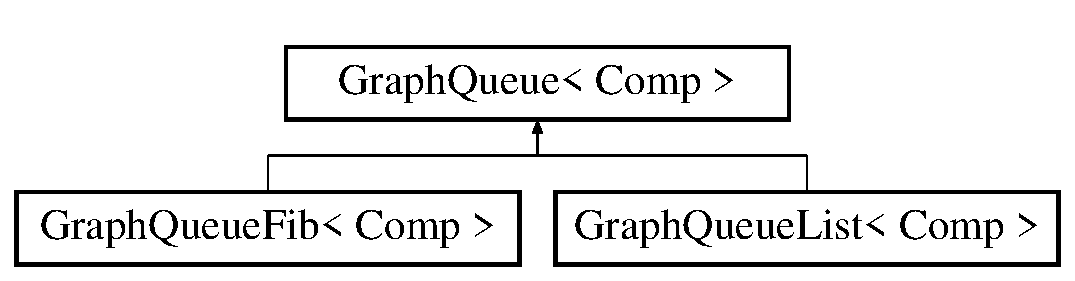
\includegraphics[height=2.000000cm]{class_graph_queue}
\end{center}
\end{figure}
\subsection*{Public Member Functions}
\begin{DoxyCompactItemize}
\item 
virtual void \hyperlink{class_graph_queue_ae29f8312580139ff26acc47b185ef946}{reset} (int num\+Vertices)=0
\begin{DoxyCompactList}\small\item\em reset the queue \end{DoxyCompactList}\item 
virtual int \hyperlink{class_graph_queue_a3fc6e39f16b7d44cd4a2e7d10f320eb8}{size} ()=0
\begin{DoxyCompactList}\small\item\em get the size of the queue \end{DoxyCompactList}\item 
virtual void \hyperlink{class_graph_queue_a613b3e0e0f4efe16abfc7c1e4c9ebe2a}{push} (\hyperlink{class_vertex}{Vertex} $\ast$v)=0
\begin{DoxyCompactList}\small\item\em add vertex to the queue \end{DoxyCompactList}\item 
virtual \hyperlink{class_vertex}{Vertex} $\ast$ \hyperlink{class_graph_queue_a81b7e172ff17a06ce84a679ff80b6a16}{top} () const =0
\begin{DoxyCompactList}\small\item\em get the highest priority vertex in queue \end{DoxyCompactList}\item 
virtual \hyperlink{class_vertex}{Vertex} $\ast$ \hyperlink{class_graph_queue_a6b6b42957573d03686dbaaa14893b9d4}{pop} ()=0
\begin{DoxyCompactList}\small\item\em remove highest priority vertex in queu \end{DoxyCompactList}\item 
virtual void \hyperlink{class_graph_queue_ae6bace12508bbbbd86a594a2ca8b9e30}{increase} (\hyperlink{class_vertex}{Vertex} $\ast$v)=0
\begin{DoxyCompactList}\small\item\em increase priority of vertex in queue \end{DoxyCompactList}\end{DoxyCompactItemize}


\subsection{Detailed Description}
\subsubsection*{template$<$class Comp$>$class Graph\+Queue$<$ Comp $>$}

generic inteface to be used in algorithms, allows the underlying data structure to switched dynamically 

\subsection{Member Function Documentation}
\hypertarget{class_graph_queue_ae6bace12508bbbbd86a594a2ca8b9e30}{}\index{Graph\+Queue@{Graph\+Queue}!increase@{increase}}
\index{increase@{increase}!Graph\+Queue@{Graph\+Queue}}
\subsubsection[{increase}]{\setlength{\rightskip}{0pt plus 5cm}template$<$class Comp$>$ virtual void {\bf Graph\+Queue}$<$ Comp $>$\+::increase (
\begin{DoxyParamCaption}
\item[{{\bf Vertex} $\ast$}]{v}
\end{DoxyParamCaption}
)\hspace{0.3cm}{\ttfamily [pure virtual]}}\label{class_graph_queue_ae6bace12508bbbbd86a594a2ca8b9e30}


increase priority of vertex in queue 


\begin{DoxyParams}{Parameters}
{\em v} & vertex to increase \\
\hline
\end{DoxyParams}


Implemented in \hyperlink{class_graph_queue_fib_a9c1a2e35ab5a0a02dc527a29c935eda7}{Graph\+Queue\+Fib$<$ Comp $>$}, and \hyperlink{class_graph_queue_list_a27345d639d6719d91c552345d400f5f6}{Graph\+Queue\+List$<$ Comp $>$}.

\hypertarget{class_graph_queue_a6b6b42957573d03686dbaaa14893b9d4}{}\index{Graph\+Queue@{Graph\+Queue}!pop@{pop}}
\index{pop@{pop}!Graph\+Queue@{Graph\+Queue}}
\subsubsection[{pop}]{\setlength{\rightskip}{0pt plus 5cm}template$<$class Comp$>$ virtual {\bf Vertex}$\ast$ {\bf Graph\+Queue}$<$ Comp $>$\+::pop (
\begin{DoxyParamCaption}
{}
\end{DoxyParamCaption}
)\hspace{0.3cm}{\ttfamily [pure virtual]}}\label{class_graph_queue_a6b6b42957573d03686dbaaa14893b9d4}


remove highest priority vertex in queu 

\begin{DoxyReturn}{Returns}
highest priority vertex in queue 
\end{DoxyReturn}


Implemented in \hyperlink{class_graph_queue_fib_ae0ab49ac553d1872c9cc7da0790b0ee3}{Graph\+Queue\+Fib$<$ Comp $>$}, and \hyperlink{class_graph_queue_list_a17fc1e6582e763755c6b174a44ccd8ec}{Graph\+Queue\+List$<$ Comp $>$}.

\hypertarget{class_graph_queue_a613b3e0e0f4efe16abfc7c1e4c9ebe2a}{}\index{Graph\+Queue@{Graph\+Queue}!push@{push}}
\index{push@{push}!Graph\+Queue@{Graph\+Queue}}
\subsubsection[{push}]{\setlength{\rightskip}{0pt plus 5cm}template$<$class Comp$>$ virtual void {\bf Graph\+Queue}$<$ Comp $>$\+::push (
\begin{DoxyParamCaption}
\item[{{\bf Vertex} $\ast$}]{v}
\end{DoxyParamCaption}
)\hspace{0.3cm}{\ttfamily [pure virtual]}}\label{class_graph_queue_a613b3e0e0f4efe16abfc7c1e4c9ebe2a}


add vertex to the queue 


\begin{DoxyParams}{Parameters}
{\em v} & vertex to add \\
\hline
\end{DoxyParams}


Implemented in \hyperlink{class_graph_queue_fib_adbf6c8d5e43cfcb5cedc2fcce60c643a}{Graph\+Queue\+Fib$<$ Comp $>$}, and \hyperlink{class_graph_queue_list_aeb2202e70dd2e556e7507327bd8824e9}{Graph\+Queue\+List$<$ Comp $>$}.

\hypertarget{class_graph_queue_ae29f8312580139ff26acc47b185ef946}{}\index{Graph\+Queue@{Graph\+Queue}!reset@{reset}}
\index{reset@{reset}!Graph\+Queue@{Graph\+Queue}}
\subsubsection[{reset}]{\setlength{\rightskip}{0pt plus 5cm}template$<$class Comp$>$ virtual void {\bf Graph\+Queue}$<$ Comp $>$\+::reset (
\begin{DoxyParamCaption}
\item[{int}]{num\+Vertices}
\end{DoxyParamCaption}
)\hspace{0.3cm}{\ttfamily [pure virtual]}}\label{class_graph_queue_ae29f8312580139ff26acc47b185ef946}


reset the queue 


\begin{DoxyParams}{Parameters}
{\em num\+Vertices} & number of vertices of grah the structure will be used on \\
\hline
\end{DoxyParams}


Implemented in \hyperlink{class_graph_queue_fib_a121fe18933b525f9c3d6aed394e9a69c}{Graph\+Queue\+Fib$<$ Comp $>$}, and \hyperlink{class_graph_queue_list_af404c9018114e84516ac28a3eeeee853}{Graph\+Queue\+List$<$ Comp $>$}.

\hypertarget{class_graph_queue_a3fc6e39f16b7d44cd4a2e7d10f320eb8}{}\index{Graph\+Queue@{Graph\+Queue}!size@{size}}
\index{size@{size}!Graph\+Queue@{Graph\+Queue}}
\subsubsection[{size}]{\setlength{\rightskip}{0pt plus 5cm}template$<$class Comp$>$ virtual int {\bf Graph\+Queue}$<$ Comp $>$\+::size (
\begin{DoxyParamCaption}
{}
\end{DoxyParamCaption}
)\hspace{0.3cm}{\ttfamily [pure virtual]}}\label{class_graph_queue_a3fc6e39f16b7d44cd4a2e7d10f320eb8}


get the size of the queue 

\begin{DoxyReturn}{Returns}
number of elements in queue 
\end{DoxyReturn}


Implemented in \hyperlink{class_graph_queue_fib_a0ce2194cd1779da1f22551f5e0ffd0f2}{Graph\+Queue\+Fib$<$ Comp $>$}, and \hyperlink{class_graph_queue_list_afc858c2e41de40db8f7b217890cfc75c}{Graph\+Queue\+List$<$ Comp $>$}.

\hypertarget{class_graph_queue_a81b7e172ff17a06ce84a679ff80b6a16}{}\index{Graph\+Queue@{Graph\+Queue}!top@{top}}
\index{top@{top}!Graph\+Queue@{Graph\+Queue}}
\subsubsection[{top}]{\setlength{\rightskip}{0pt plus 5cm}template$<$class Comp$>$ virtual {\bf Vertex}$\ast$ {\bf Graph\+Queue}$<$ Comp $>$\+::top (
\begin{DoxyParamCaption}
{}
\end{DoxyParamCaption}
) const\hspace{0.3cm}{\ttfamily [pure virtual]}}\label{class_graph_queue_a81b7e172ff17a06ce84a679ff80b6a16}


get the highest priority vertex in queue 

\begin{DoxyReturn}{Returns}
highest priority vertex in queue 
\end{DoxyReturn}


Implemented in \hyperlink{class_graph_queue_fib_a3b1b6a0bf8007559ba3f66978413845c}{Graph\+Queue\+Fib$<$ Comp $>$}, and \hyperlink{class_graph_queue_list_a56493dd03e8378a67033eaba8c71d9ea}{Graph\+Queue\+List$<$ Comp $>$}.



The documentation for this class was generated from the following file\+:\begin{DoxyCompactItemize}
\item 
C\+:/\+Users/\+André/\+Desktop/test/algorithms/Graph\+Queue.\+h\end{DoxyCompactItemize}

\hypertarget{class_graph_queue_fib}{}\section{Graph\+Queue\+Fib$<$ Comp $>$ Class Template Reference}
\label{class_graph_queue_fib}\index{Graph\+Queue\+Fib$<$ Comp $>$@{Graph\+Queue\+Fib$<$ Comp $>$}}


Implements Fibonacci\+Heaps able to be used with the algorithm\textquotesingle{}s template.  




{\ttfamily \#include $<$Graph\+Queue\+Fib.\+h$>$}

Inheritance diagram for Graph\+Queue\+Fib$<$ Comp $>$\+:\begin{figure}[H]
\begin{center}
\leavevmode
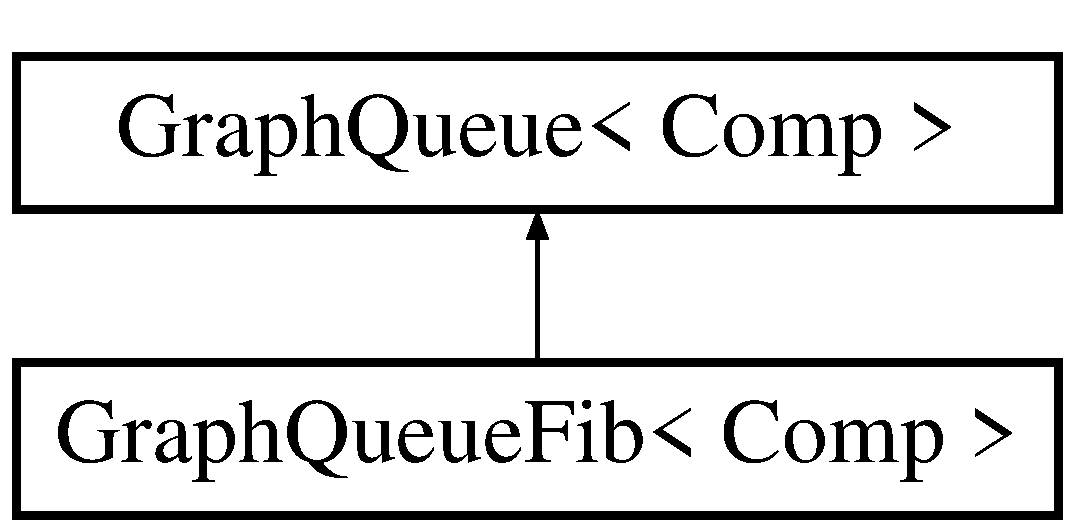
\includegraphics[height=2.000000cm]{class_graph_queue_fib}
\end{center}
\end{figure}
\subsection*{Public Member Functions}
\begin{DoxyCompactItemize}
\item 
\hyperlink{class_graph_queue_fib_ac6d57ed1a0dc58f986aea1a1d149a154}{Graph\+Queue\+Fib} (int num\+Vertices)
\begin{DoxyCompactList}\small\item\em queue constructor \end{DoxyCompactList}\item 
void \hyperlink{class_graph_queue_fib_adbf6c8d5e43cfcb5cedc2fcce60c643a}{push} (\hyperlink{class_vertex}{Vertex} $\ast$v)
\begin{DoxyCompactList}\small\item\em add vertex to the queue \end{DoxyCompactList}\item 
\hyperlink{class_vertex}{Vertex} $\ast$ \hyperlink{class_graph_queue_fib_a3b1b6a0bf8007559ba3f66978413845c}{top} () const 
\begin{DoxyCompactList}\small\item\em get the highest priority vertex in queue \end{DoxyCompactList}\item 
\hyperlink{class_vertex}{Vertex} $\ast$ \hyperlink{class_graph_queue_fib_ae0ab49ac553d1872c9cc7da0790b0ee3}{pop} ()
\begin{DoxyCompactList}\small\item\em remove highest priority vertex in queu \end{DoxyCompactList}\item 
void \hyperlink{class_graph_queue_fib_a9c1a2e35ab5a0a02dc527a29c935eda7}{increase} (\hyperlink{class_vertex}{Vertex} $\ast$v)
\begin{DoxyCompactList}\small\item\em increase priority of vertex in queue \end{DoxyCompactList}\item 
void \hyperlink{class_graph_queue_fib_a121fe18933b525f9c3d6aed394e9a69c}{reset} (int num\+Vertices)
\begin{DoxyCompactList}\small\item\em reset the queue \end{DoxyCompactList}\item 
int \hyperlink{class_graph_queue_fib_a0ce2194cd1779da1f22551f5e0ffd0f2}{size} ()
\begin{DoxyCompactList}\small\item\em get the size of the queue \end{DoxyCompactList}\end{DoxyCompactItemize}


\subsection{Detailed Description}
\subsubsection*{template$<$class Comp$>$class Graph\+Queue\+Fib$<$ Comp $>$}

Implements Fibonacci\+Heaps able to be used with the algorithm\textquotesingle{}s template. 

\subsection{Constructor \& Destructor Documentation}
\hypertarget{class_graph_queue_fib_ac6d57ed1a0dc58f986aea1a1d149a154}{}\index{Graph\+Queue\+Fib@{Graph\+Queue\+Fib}!Graph\+Queue\+Fib@{Graph\+Queue\+Fib}}
\index{Graph\+Queue\+Fib@{Graph\+Queue\+Fib}!Graph\+Queue\+Fib@{Graph\+Queue\+Fib}}
\subsubsection[{Graph\+Queue\+Fib}]{\setlength{\rightskip}{0pt plus 5cm}template$<$class Comp $>$ {\bf Graph\+Queue\+Fib}$<$ Comp $>$\+::{\bf Graph\+Queue\+Fib} (
\begin{DoxyParamCaption}
\item[{int}]{num\+Vertices}
\end{DoxyParamCaption}
)}\label{class_graph_queue_fib_ac6d57ed1a0dc58f986aea1a1d149a154}


queue constructor 


\begin{DoxyParams}{Parameters}
{\em num\+Vertices} & number of vertices of grah the structure will be used on \\
\hline
\end{DoxyParams}


\subsection{Member Function Documentation}
\hypertarget{class_graph_queue_fib_a9c1a2e35ab5a0a02dc527a29c935eda7}{}\index{Graph\+Queue\+Fib@{Graph\+Queue\+Fib}!increase@{increase}}
\index{increase@{increase}!Graph\+Queue\+Fib@{Graph\+Queue\+Fib}}
\subsubsection[{increase}]{\setlength{\rightskip}{0pt plus 5cm}template$<$class Comp $>$ void {\bf Graph\+Queue\+Fib}$<$ Comp $>$\+::increase (
\begin{DoxyParamCaption}
\item[{{\bf Vertex} $\ast$}]{v}
\end{DoxyParamCaption}
)\hspace{0.3cm}{\ttfamily [virtual]}}\label{class_graph_queue_fib_a9c1a2e35ab5a0a02dc527a29c935eda7}


increase priority of vertex in queue 


\begin{DoxyParams}{Parameters}
{\em v} & vertex to increase \\
\hline
\end{DoxyParams}


Implements \hyperlink{class_graph_queue_ae6bace12508bbbbd86a594a2ca8b9e30}{Graph\+Queue$<$ Comp $>$}.

\hypertarget{class_graph_queue_fib_ae0ab49ac553d1872c9cc7da0790b0ee3}{}\index{Graph\+Queue\+Fib@{Graph\+Queue\+Fib}!pop@{pop}}
\index{pop@{pop}!Graph\+Queue\+Fib@{Graph\+Queue\+Fib}}
\subsubsection[{pop}]{\setlength{\rightskip}{0pt plus 5cm}template$<$class Comp $>$ {\bf Vertex} $\ast$ {\bf Graph\+Queue\+Fib}$<$ Comp $>$\+::pop (
\begin{DoxyParamCaption}
{}
\end{DoxyParamCaption}
)\hspace{0.3cm}{\ttfamily [virtual]}}\label{class_graph_queue_fib_ae0ab49ac553d1872c9cc7da0790b0ee3}


remove highest priority vertex in queu 

\begin{DoxyReturn}{Returns}
highest priority vertex in queue 
\end{DoxyReturn}


Implements \hyperlink{class_graph_queue_a6b6b42957573d03686dbaaa14893b9d4}{Graph\+Queue$<$ Comp $>$}.

\hypertarget{class_graph_queue_fib_adbf6c8d5e43cfcb5cedc2fcce60c643a}{}\index{Graph\+Queue\+Fib@{Graph\+Queue\+Fib}!push@{push}}
\index{push@{push}!Graph\+Queue\+Fib@{Graph\+Queue\+Fib}}
\subsubsection[{push}]{\setlength{\rightskip}{0pt plus 5cm}template$<$class Comp $>$ void {\bf Graph\+Queue\+Fib}$<$ Comp $>$\+::push (
\begin{DoxyParamCaption}
\item[{{\bf Vertex} $\ast$}]{v}
\end{DoxyParamCaption}
)\hspace{0.3cm}{\ttfamily [virtual]}}\label{class_graph_queue_fib_adbf6c8d5e43cfcb5cedc2fcce60c643a}


add vertex to the queue 


\begin{DoxyParams}{Parameters}
{\em v} & vertex to add \\
\hline
\end{DoxyParams}


Implements \hyperlink{class_graph_queue_a613b3e0e0f4efe16abfc7c1e4c9ebe2a}{Graph\+Queue$<$ Comp $>$}.

\hypertarget{class_graph_queue_fib_a121fe18933b525f9c3d6aed394e9a69c}{}\index{Graph\+Queue\+Fib@{Graph\+Queue\+Fib}!reset@{reset}}
\index{reset@{reset}!Graph\+Queue\+Fib@{Graph\+Queue\+Fib}}
\subsubsection[{reset}]{\setlength{\rightskip}{0pt plus 5cm}template$<$class Comp $>$ void {\bf Graph\+Queue\+Fib}$<$ Comp $>$\+::reset (
\begin{DoxyParamCaption}
\item[{int}]{num\+Vertices}
\end{DoxyParamCaption}
)\hspace{0.3cm}{\ttfamily [virtual]}}\label{class_graph_queue_fib_a121fe18933b525f9c3d6aed394e9a69c}


reset the queue 


\begin{DoxyParams}{Parameters}
{\em num\+Vertices} & number of vertices of grah the structure will be used on \\
\hline
\end{DoxyParams}


Implements \hyperlink{class_graph_queue_ae29f8312580139ff26acc47b185ef946}{Graph\+Queue$<$ Comp $>$}.

\hypertarget{class_graph_queue_fib_a0ce2194cd1779da1f22551f5e0ffd0f2}{}\index{Graph\+Queue\+Fib@{Graph\+Queue\+Fib}!size@{size}}
\index{size@{size}!Graph\+Queue\+Fib@{Graph\+Queue\+Fib}}
\subsubsection[{size}]{\setlength{\rightskip}{0pt plus 5cm}template$<$class Comp $>$ int {\bf Graph\+Queue\+Fib}$<$ Comp $>$\+::size (
\begin{DoxyParamCaption}
{}
\end{DoxyParamCaption}
)\hspace{0.3cm}{\ttfamily [virtual]}}\label{class_graph_queue_fib_a0ce2194cd1779da1f22551f5e0ffd0f2}


get the size of the queue 

\begin{DoxyReturn}{Returns}
number of elements in queue 
\end{DoxyReturn}


Implements \hyperlink{class_graph_queue_a3fc6e39f16b7d44cd4a2e7d10f320eb8}{Graph\+Queue$<$ Comp $>$}.

\hypertarget{class_graph_queue_fib_a3b1b6a0bf8007559ba3f66978413845c}{}\index{Graph\+Queue\+Fib@{Graph\+Queue\+Fib}!top@{top}}
\index{top@{top}!Graph\+Queue\+Fib@{Graph\+Queue\+Fib}}
\subsubsection[{top}]{\setlength{\rightskip}{0pt plus 5cm}template$<$class Comp $>$ {\bf Vertex} $\ast$ {\bf Graph\+Queue\+Fib}$<$ Comp $>$\+::top (
\begin{DoxyParamCaption}
{}
\end{DoxyParamCaption}
) const\hspace{0.3cm}{\ttfamily [virtual]}}\label{class_graph_queue_fib_a3b1b6a0bf8007559ba3f66978413845c}


get the highest priority vertex in queue 

\begin{DoxyReturn}{Returns}
highest priority vertex in queue 
\end{DoxyReturn}


Implements \hyperlink{class_graph_queue_a81b7e172ff17a06ce84a679ff80b6a16}{Graph\+Queue$<$ Comp $>$}.



The documentation for this class was generated from the following file\+:\begin{DoxyCompactItemize}
\item 
C\+:/\+Users/\+André/\+Desktop/test/algorithms/Graph\+Queue\+Fib.\+h\end{DoxyCompactItemize}

\hypertarget{class_graph_queue_list}{}\section{Graph\+Queue\+List$<$ Comp $>$ Class Template Reference}
\label{class_graph_queue_list}\index{Graph\+Queue\+List$<$ Comp $>$@{Graph\+Queue\+List$<$ Comp $>$}}


Implements a list able to be used with the algorithm\textquotesingle{}s template.  




{\ttfamily \#include $<$Graph\+Queue\+List.\+h$>$}

Inheritance diagram for Graph\+Queue\+List$<$ Comp $>$\+:\begin{figure}[H]
\begin{center}
\leavevmode
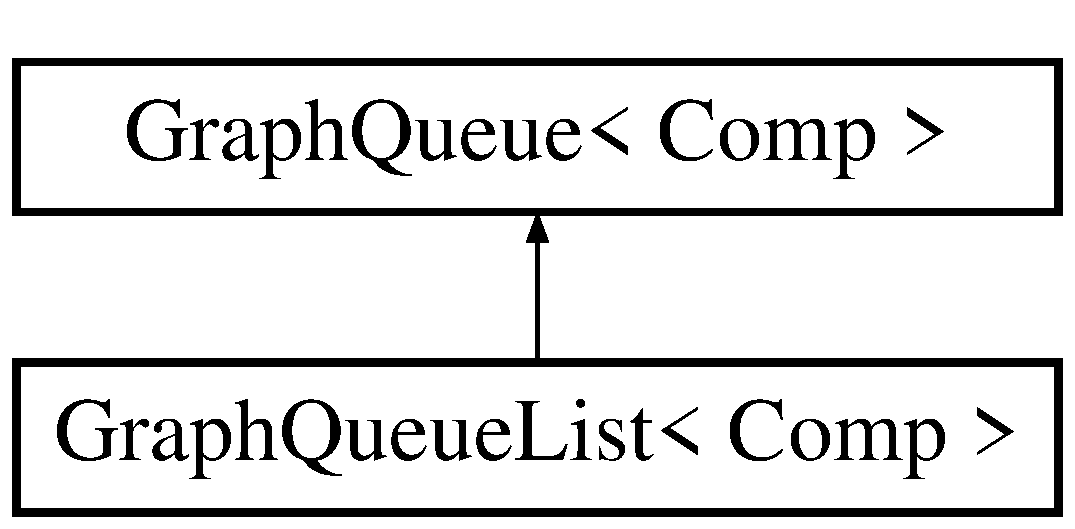
\includegraphics[height=2.000000cm]{class_graph_queue_list}
\end{center}
\end{figure}
\subsection*{Public Member Functions}
\begin{DoxyCompactItemize}
\item 
\hyperlink{class_graph_queue_list_a61c2e8ecb3fe52fca17dd84216f356a0}{Graph\+Queue\+List} (int num\+Vertices)
\begin{DoxyCompactList}\small\item\em queue constructor \end{DoxyCompactList}\item 
void \hyperlink{class_graph_queue_list_aeb2202e70dd2e556e7507327bd8824e9}{push} (\hyperlink{class_vertex}{Vertex} $\ast$v)
\begin{DoxyCompactList}\small\item\em add vertex to the queue \end{DoxyCompactList}\item 
\hyperlink{class_vertex}{Vertex} $\ast$ \hyperlink{class_graph_queue_list_a56493dd03e8378a67033eaba8c71d9ea}{top} () const 
\begin{DoxyCompactList}\small\item\em get the highest priority vertex in queue \end{DoxyCompactList}\item 
\hyperlink{class_vertex}{Vertex} $\ast$ \hyperlink{class_graph_queue_list_a17fc1e6582e763755c6b174a44ccd8ec}{pop} ()
\begin{DoxyCompactList}\small\item\em remove highest priority vertex in queu \end{DoxyCompactList}\item 
void \hyperlink{class_graph_queue_list_a27345d639d6719d91c552345d400f5f6}{increase} (\hyperlink{class_vertex}{Vertex} $\ast$v)
\begin{DoxyCompactList}\small\item\em increase priority of vertex in queue \end{DoxyCompactList}\item 
void \hyperlink{class_graph_queue_list_af404c9018114e84516ac28a3eeeee853}{reset} (int num\+Vertices)
\begin{DoxyCompactList}\small\item\em reset the queue \end{DoxyCompactList}\item 
int \hyperlink{class_graph_queue_list_afc858c2e41de40db8f7b217890cfc75c}{size} ()
\begin{DoxyCompactList}\small\item\em get the size of the queue \end{DoxyCompactList}\end{DoxyCompactItemize}


\subsection{Detailed Description}
\subsubsection*{template$<$class Comp$>$class Graph\+Queue\+List$<$ Comp $>$}

Implements a list able to be used with the algorithm\textquotesingle{}s template. 

\subsection{Constructor \& Destructor Documentation}
\hypertarget{class_graph_queue_list_a61c2e8ecb3fe52fca17dd84216f356a0}{}\index{Graph\+Queue\+List@{Graph\+Queue\+List}!Graph\+Queue\+List@{Graph\+Queue\+List}}
\index{Graph\+Queue\+List@{Graph\+Queue\+List}!Graph\+Queue\+List@{Graph\+Queue\+List}}
\subsubsection[{Graph\+Queue\+List}]{\setlength{\rightskip}{0pt plus 5cm}template$<$class Comp $>$ {\bf Graph\+Queue\+List}$<$ Comp $>$\+::{\bf Graph\+Queue\+List} (
\begin{DoxyParamCaption}
\item[{int}]{num\+Vertices}
\end{DoxyParamCaption}
)}\label{class_graph_queue_list_a61c2e8ecb3fe52fca17dd84216f356a0}


queue constructor 


\begin{DoxyParams}{Parameters}
{\em num\+Vertices} & number of vertices of grah the structure will be used on \\
\hline
\end{DoxyParams}


\subsection{Member Function Documentation}
\hypertarget{class_graph_queue_list_a27345d639d6719d91c552345d400f5f6}{}\index{Graph\+Queue\+List@{Graph\+Queue\+List}!increase@{increase}}
\index{increase@{increase}!Graph\+Queue\+List@{Graph\+Queue\+List}}
\subsubsection[{increase}]{\setlength{\rightskip}{0pt plus 5cm}template$<$class Comp $>$ void {\bf Graph\+Queue\+List}$<$ Comp $>$\+::increase (
\begin{DoxyParamCaption}
\item[{{\bf Vertex} $\ast$}]{v}
\end{DoxyParamCaption}
)\hspace{0.3cm}{\ttfamily [virtual]}}\label{class_graph_queue_list_a27345d639d6719d91c552345d400f5f6}


increase priority of vertex in queue 


\begin{DoxyParams}{Parameters}
{\em v} & vertex to increase \\
\hline
\end{DoxyParams}


Implements \hyperlink{class_graph_queue_ae6bace12508bbbbd86a594a2ca8b9e30}{Graph\+Queue$<$ Comp $>$}.

\hypertarget{class_graph_queue_list_a17fc1e6582e763755c6b174a44ccd8ec}{}\index{Graph\+Queue\+List@{Graph\+Queue\+List}!pop@{pop}}
\index{pop@{pop}!Graph\+Queue\+List@{Graph\+Queue\+List}}
\subsubsection[{pop}]{\setlength{\rightskip}{0pt plus 5cm}template$<$class Comp $>$ {\bf Vertex} $\ast$ {\bf Graph\+Queue\+List}$<$ Comp $>$\+::pop (
\begin{DoxyParamCaption}
{}
\end{DoxyParamCaption}
)\hspace{0.3cm}{\ttfamily [virtual]}}\label{class_graph_queue_list_a17fc1e6582e763755c6b174a44ccd8ec}


remove highest priority vertex in queu 

\begin{DoxyReturn}{Returns}
highest priority vertex in queue 
\end{DoxyReturn}


Implements \hyperlink{class_graph_queue_a6b6b42957573d03686dbaaa14893b9d4}{Graph\+Queue$<$ Comp $>$}.

\hypertarget{class_graph_queue_list_aeb2202e70dd2e556e7507327bd8824e9}{}\index{Graph\+Queue\+List@{Graph\+Queue\+List}!push@{push}}
\index{push@{push}!Graph\+Queue\+List@{Graph\+Queue\+List}}
\subsubsection[{push}]{\setlength{\rightskip}{0pt plus 5cm}template$<$class Comp $>$ void {\bf Graph\+Queue\+List}$<$ Comp $>$\+::push (
\begin{DoxyParamCaption}
\item[{{\bf Vertex} $\ast$}]{v}
\end{DoxyParamCaption}
)\hspace{0.3cm}{\ttfamily [virtual]}}\label{class_graph_queue_list_aeb2202e70dd2e556e7507327bd8824e9}


add vertex to the queue 


\begin{DoxyParams}{Parameters}
{\em v} & vertex to add \\
\hline
\end{DoxyParams}


Implements \hyperlink{class_graph_queue_a613b3e0e0f4efe16abfc7c1e4c9ebe2a}{Graph\+Queue$<$ Comp $>$}.

\hypertarget{class_graph_queue_list_af404c9018114e84516ac28a3eeeee853}{}\index{Graph\+Queue\+List@{Graph\+Queue\+List}!reset@{reset}}
\index{reset@{reset}!Graph\+Queue\+List@{Graph\+Queue\+List}}
\subsubsection[{reset}]{\setlength{\rightskip}{0pt plus 5cm}template$<$class Comp $>$ void {\bf Graph\+Queue\+List}$<$ Comp $>$\+::reset (
\begin{DoxyParamCaption}
\item[{int}]{num\+Vertices}
\end{DoxyParamCaption}
)\hspace{0.3cm}{\ttfamily [virtual]}}\label{class_graph_queue_list_af404c9018114e84516ac28a3eeeee853}


reset the queue 


\begin{DoxyParams}{Parameters}
{\em num\+Vertices} & number of vertices of grah the structure will be used on \\
\hline
\end{DoxyParams}


Implements \hyperlink{class_graph_queue_ae29f8312580139ff26acc47b185ef946}{Graph\+Queue$<$ Comp $>$}.

\hypertarget{class_graph_queue_list_afc858c2e41de40db8f7b217890cfc75c}{}\index{Graph\+Queue\+List@{Graph\+Queue\+List}!size@{size}}
\index{size@{size}!Graph\+Queue\+List@{Graph\+Queue\+List}}
\subsubsection[{size}]{\setlength{\rightskip}{0pt plus 5cm}template$<$class Comp $>$ int {\bf Graph\+Queue\+List}$<$ Comp $>$\+::size (
\begin{DoxyParamCaption}
{}
\end{DoxyParamCaption}
)\hspace{0.3cm}{\ttfamily [virtual]}}\label{class_graph_queue_list_afc858c2e41de40db8f7b217890cfc75c}


get the size of the queue 

\begin{DoxyReturn}{Returns}
number of elements in queue 
\end{DoxyReturn}


Implements \hyperlink{class_graph_queue_a3fc6e39f16b7d44cd4a2e7d10f320eb8}{Graph\+Queue$<$ Comp $>$}.

\hypertarget{class_graph_queue_list_a56493dd03e8378a67033eaba8c71d9ea}{}\index{Graph\+Queue\+List@{Graph\+Queue\+List}!top@{top}}
\index{top@{top}!Graph\+Queue\+List@{Graph\+Queue\+List}}
\subsubsection[{top}]{\setlength{\rightskip}{0pt plus 5cm}template$<$class Comp $>$ {\bf Vertex} $\ast$ {\bf Graph\+Queue\+List}$<$ Comp $>$\+::top (
\begin{DoxyParamCaption}
{}
\end{DoxyParamCaption}
) const\hspace{0.3cm}{\ttfamily [virtual]}}\label{class_graph_queue_list_a56493dd03e8378a67033eaba8c71d9ea}


get the highest priority vertex in queue 

\begin{DoxyReturn}{Returns}
highest priority vertex in queue 
\end{DoxyReturn}


Implements \hyperlink{class_graph_queue_a81b7e172ff17a06ce84a679ff80b6a16}{Graph\+Queue$<$ Comp $>$}.



The documentation for this class was generated from the following file\+:\begin{DoxyCompactItemize}
\item 
C\+:/\+Users/\+André/\+Desktop/test/algorithms/Graph\+Queue\+List.\+h\end{DoxyCompactItemize}

\hypertarget{class_hour}{}\section{Hour Class Reference}
\label{class_hour}\index{Hour@{Hour}}


Interface for a hour-\/minute-\/second timestamp.  




{\ttfamily \#include $<$Hour.\+h$>$}

\subsection*{Public Member Functions}
\begin{DoxyCompactItemize}
\item 
\hyperlink{class_hour_a596868e9c3802335f81f538efc0911f3}{Hour} (const std\+::string \&hour)
\begin{DoxyCompactList}\small\item\em construct hour object from a string \end{DoxyCompactList}\item 
\hypertarget{class_hour_a2fd12606e010fc8a07af09de5cd28d83}{}{\bfseries Hour} (unsigned seconds)\label{class_hour_a2fd12606e010fc8a07af09de5cd28d83}

\item 
\hyperlink{class_hour_a3da244a601fba002d20eb9a7de724574}{Hour} (unsigned hours, unsigned minutes, unsigned seconds=0)
\begin{DoxyCompactList}\small\item\em construct hour object from a number of hours, minutes and seconds \end{DoxyCompactList}\item 
\hypertarget{class_hour_aa370ac8ba17cf52dc7f00e6f3b529c2b}{}unsigned \hyperlink{class_hour_aa370ac8ba17cf52dc7f00e6f3b529c2b}{get\+Hourstamp} () const \label{class_hour_aa370ac8ba17cf52dc7f00e6f3b529c2b}

\begin{DoxyCompactList}\small\item\em get the number of seconds \end{DoxyCompactList}\item 
\hypertarget{class_hour_a4aa915a1163bfbc028d2e31a6a8a3b90}{}void {\bfseries set\+Hourstamp} (unsigned hourstamp)\label{class_hour_a4aa915a1163bfbc028d2e31a6a8a3b90}

\item 
\hypertarget{class_hour_a07e78b2131a713ec25f88c459032987c}{}\hyperlink{class_hour}{Hour} \& {\bfseries operator+=} (const \hyperlink{class_hour}{Hour} \&hour)\label{class_hour_a07e78b2131a713ec25f88c459032987c}

\item 
\hypertarget{class_hour_a4883bfa83e28707fc3088bba441fcecd}{}\hyperlink{class_hour}{Hour} {\bfseries operator+} (const \hyperlink{class_hour}{Hour} \&hour) const \label{class_hour_a4883bfa83e28707fc3088bba441fcecd}

\item 
\hypertarget{class_hour_a9e38c8fb275a7c298889be34f706573a}{}\hyperlink{class_hour}{Hour} \& {\bfseries operator-\/=} (const \hyperlink{class_hour}{Hour} \&hour)\label{class_hour_a9e38c8fb275a7c298889be34f706573a}

\item 
\hypertarget{class_hour_a7a8530d730ee3cf31523543bd0af2508}{}\hyperlink{class_hour}{Hour} {\bfseries operator-\/} (const \hyperlink{class_hour}{Hour} \&hour) const \label{class_hour_a7a8530d730ee3cf31523543bd0af2508}

\item 
\hypertarget{class_hour_ae0122e41355427701ff951470432e7bd}{}\hyperlink{class_hour}{Hour} \& {\bfseries operator/=} (double quocient)\label{class_hour_ae0122e41355427701ff951470432e7bd}

\item 
\hypertarget{class_hour_a593c1d0d96ddf7ac7f0ce786a0865955}{}\hyperlink{class_hour}{Hour} {\bfseries operator/} (double quocient) const \label{class_hour_a593c1d0d96ddf7ac7f0ce786a0865955}

\item 
\hypertarget{class_hour_a208b4071e81037cf9c65a385cff0beb4}{}bool {\bfseries operator$<$} (const \hyperlink{class_hour}{Hour} \&hour) const \label{class_hour_a208b4071e81037cf9c65a385cff0beb4}

\item 
\hypertarget{class_hour_a1e97cf9ea7a47499516c62462af7c4a2}{}bool {\bfseries operator$>$} (const \hyperlink{class_hour}{Hour} \&hour) const \label{class_hour_a1e97cf9ea7a47499516c62462af7c4a2}

\end{DoxyCompactItemize}
\subsection*{Static Public Attributes}
\begin{DoxyCompactItemize}
\item 
\hypertarget{class_hour_a564c0da9badbb2e51b882f5655fc4cff}{}static const unsigned {\bfseries seconds\+Per\+Minute} = 60\label{class_hour_a564c0da9badbb2e51b882f5655fc4cff}

\item 
\hypertarget{class_hour_accca3564855b553925b64af70ee735a8}{}static const unsigned {\bfseries minutes\+Per\+Hour} = 60\label{class_hour_accca3564855b553925b64af70ee735a8}

\item 
\hypertarget{class_hour_a03cdb980e42ccbe6897559ff28c51439}{}static const unsigned {\bfseries hours\+Per\+Day} = 24\label{class_hour_a03cdb980e42ccbe6897559ff28c51439}

\item 
\hypertarget{class_hour_aebe16a850ba082b7b5a056ac41aaade9}{}static const unsigned {\bfseries minutes\+Per\+Day} = Hour\+::hours\+Per\+Day $\ast$ Hour\+::minutes\+Per\+Hour\label{class_hour_aebe16a850ba082b7b5a056ac41aaade9}

\item 
\hypertarget{class_hour_af4843be5f00f94cf53ce1770d15d4b77}{}static const unsigned {\bfseries seconds\+Per\+Day} = Hour\+::minutes\+Per\+Day $\ast$ Hour\+::seconds\+Per\+Minute\label{class_hour_af4843be5f00f94cf53ce1770d15d4b77}

\item 
\hypertarget{class_hour_aedcfa9fbea1342493ba563723a01b37c}{}static const unsigned {\bfseries seconds\+Per\+Hour} = Hour\+::minutes\+Per\+Hour $\ast$ Hour\+::seconds\+Per\+Minute\label{class_hour_aedcfa9fbea1342493ba563723a01b37c}

\end{DoxyCompactItemize}
\subsection*{Friends}
\begin{DoxyCompactItemize}
\item 
\hypertarget{class_hour_ac4eba5ff16ebc7f457a494230cd0ac5d}{}\hyperlink{class_hour}{Hour} {\bfseries operator$\ast$} (const \hyperlink{class_hour}{Hour} \&hour, double factor)\label{class_hour_ac4eba5ff16ebc7f457a494230cd0ac5d}

\item 
\hypertarget{class_hour_a5a8828bbd135c58b3a15a30ac2e512e4}{}\hyperlink{class_hour}{Hour} {\bfseries operator+} (const \hyperlink{class_hour}{Hour} \&hour, double x)\label{class_hour_a5a8828bbd135c58b3a15a30ac2e512e4}

\item 
\hypertarget{class_hour_ad5e7eb1ac08edb6d5aad033e54136a5a}{}std\+::ostream \& {\bfseries operator$<$$<$} (std\+::ostream \&os, const \hyperlink{class_hour}{Hour} \&hour)\label{class_hour_ad5e7eb1ac08edb6d5aad033e54136a5a}

\end{DoxyCompactItemize}


\subsection{Detailed Description}
Interface for a hour-\/minute-\/second timestamp. 

\subsection{Constructor \& Destructor Documentation}
\hypertarget{class_hour_a596868e9c3802335f81f538efc0911f3}{}\index{Hour@{Hour}!Hour@{Hour}}
\index{Hour@{Hour}!Hour@{Hour}}
\subsubsection[{Hour}]{\setlength{\rightskip}{0pt plus 5cm}Hour\+::\+Hour (
\begin{DoxyParamCaption}
\item[{const std\+::string \&}]{hour}
\end{DoxyParamCaption}
)}\label{class_hour_a596868e9c3802335f81f538efc0911f3}


construct hour object from a string 


\begin{DoxyParams}{Parameters}
{\em hour} & string in format H\+H\+:M\+M \\
\hline
\end{DoxyParams}
\hypertarget{class_hour_a3da244a601fba002d20eb9a7de724574}{}\index{Hour@{Hour}!Hour@{Hour}}
\index{Hour@{Hour}!Hour@{Hour}}
\subsubsection[{Hour}]{\setlength{\rightskip}{0pt plus 5cm}Hour\+::\+Hour (
\begin{DoxyParamCaption}
\item[{unsigned}]{hours, }
\item[{unsigned}]{minutes, }
\item[{unsigned}]{seconds = {\ttfamily 0}}
\end{DoxyParamCaption}
)\hspace{0.3cm}{\ttfamily [inline]}}\label{class_hour_a3da244a601fba002d20eb9a7de724574}


construct hour object from a number of hours, minutes and seconds 


\begin{DoxyParams}{Parameters}
{\em hours} & hours \\
\hline
{\em minutes} & minutes \\
\hline
{\em seconds} & seconds (optional) \\
\hline
\end{DoxyParams}


The documentation for this class was generated from the following files\+:\begin{DoxyCompactItemize}
\item 
C\+:/\+Users/\+André/\+Desktop/test/transport/Hour.\+h\item 
C\+:/\+Users/\+André/\+Desktop/test/transport/Hour.\+cpp\end{DoxyCompactItemize}

\hypertarget{class_map_1_1_loader_1_1_invalid_input_exception}{}\section{Map\+:\+:Loader\+:\+:Invalid\+Input\+Exception Class Reference}
\label{class_map_1_1_loader_1_1_invalid_input_exception}\index{Map\+::\+Loader\+::\+Invalid\+Input\+Exception@{Map\+::\+Loader\+::\+Invalid\+Input\+Exception}}
\subsection*{Public Member Functions}
\begin{DoxyCompactItemize}
\item 
\hypertarget{class_map_1_1_loader_1_1_invalid_input_exception_a23d2558846f42f211465f08c38191944}{}{\bfseries Invalid\+Input\+Exception} (const string \&info)\label{class_map_1_1_loader_1_1_invalid_input_exception_a23d2558846f42f211465f08c38191944}

\item 
\hypertarget{class_map_1_1_loader_1_1_invalid_input_exception_a73aacf27d8a4a1b071381ff00253f3a3}{}const string \& {\bfseries get\+Info} ()\label{class_map_1_1_loader_1_1_invalid_input_exception_a73aacf27d8a4a1b071381ff00253f3a3}

\end{DoxyCompactItemize}


The documentation for this class was generated from the following file\+:\begin{DoxyCompactItemize}
\item 
C\+:/\+Users/\+André/\+Desktop/test/transport/Map.\+h\end{DoxyCompactItemize}

\hypertarget{class_map_1_1_loader}{}\section{Map\+:\+:Loader Class Reference}
\label{class_map_1_1_loader}\index{Map\+::\+Loader@{Map\+::\+Loader}}
\subsection*{Classes}
\begin{DoxyCompactItemize}
\item 
class \hyperlink{class_map_1_1_loader_1_1_invalid_input_exception}{Invalid\+Input\+Exception}
\end{DoxyCompactItemize}
\subsection*{Public Member Functions}
\begin{DoxyCompactItemize}
\item 
\hypertarget{class_map_1_1_loader_a2cd5aceed982a568149fffb0e3786215}{}void {\bfseries load} (\hyperlink{class_map}{Map} \&map)\label{class_map_1_1_loader_a2cd5aceed982a568149fffb0e3786215}

\end{DoxyCompactItemize}


The documentation for this class was generated from the following files\+:\begin{DoxyCompactItemize}
\item 
C\+:/\+Users/\+André/\+Desktop/test/transport/Map.\+h\item 
C\+:/\+Users/\+André/\+Desktop/test/transport/Map.\+cpp\end{DoxyCompactItemize}

\hypertarget{class_map}{}\section{Map Class Reference}
\label{class_map}\index{Map@{Map}}


Abstraction to the real \char`\"{}world\char`\"{} map, able to convert it to a \hyperlink{class_graph}{Graph}.  




{\ttfamily \#include $<$Map.\+h$>$}

\subsection*{Classes}
\begin{DoxyCompactItemize}
\item 
class \hyperlink{class_map_1_1_loader}{Loader}
\end{DoxyCompactItemize}
\subsection*{Public Member Functions}
\begin{DoxyCompactItemize}
\item 
\hypertarget{class_map_a0f5ad0fd4563497b4214038cbca8b582}{}\hyperlink{class_map_a0f5ad0fd4563497b4214038cbca8b582}{Map} ()\label{class_map_a0f5ad0fd4563497b4214038cbca8b582}

\begin{DoxyCompactList}\small\item\em map construtor \end{DoxyCompactList}\item 
\hypertarget{class_map_af125f0e44cfce711a534d679f585398d}{}const std\+::vector$<$ \hyperlink{class_bus_route}{Bus\+Route} $>$ \& {\bfseries get\+Bus\+Routes} () const \label{class_map_af125f0e44cfce711a534d679f585398d}

\item 
\hypertarget{class_map_accd8e5fc6cf0bce023c49573c392e792}{}const std\+::vector$<$ \hyperlink{class_bus_stop}{Bus\+Stop} $\ast$ $>$ \& {\bfseries get\+Bus\+Stops} () const \label{class_map_accd8e5fc6cf0bce023c49573c392e792}

\item 
\hypertarget{class_map_ac235446e8626f7a71e10317549b20cbf}{}\hyperlink{class_graph}{Graph} {\bfseries generate\+Graph} () const \label{class_map_ac235446e8626f7a71e10317549b20cbf}

\end{DoxyCompactItemize}
\subsection*{Friends}
\begin{DoxyCompactItemize}
\item 
\hypertarget{class_map_ac8e5438321e35520c4088ff6ca4116ee}{}class {\bfseries Loader}\label{class_map_ac8e5438321e35520c4088ff6ca4116ee}

\end{DoxyCompactItemize}


\subsection{Detailed Description}
Abstraction to the real \char`\"{}world\char`\"{} map, able to convert it to a \hyperlink{class_graph}{Graph}. 

The documentation for this class was generated from the following files\+:\begin{DoxyCompactItemize}
\item 
C\+:/\+Users/\+André/\+Desktop/test/transport/Map.\+h\item 
C\+:/\+Users/\+André/\+Desktop/test/transport/Map.\+cpp\end{DoxyCompactItemize}

\hypertarget{class_metro_edge}{}\section{Metro\+Edge Class Reference}
\label{class_metro_edge}\index{Metro\+Edge@{Metro\+Edge}}


Connection between two metro stops.  




{\ttfamily \#include $<$Metro\+Edge.\+h$>$}

Inheritance diagram for Metro\+Edge\+:\begin{figure}[H]
\begin{center}
\leavevmode
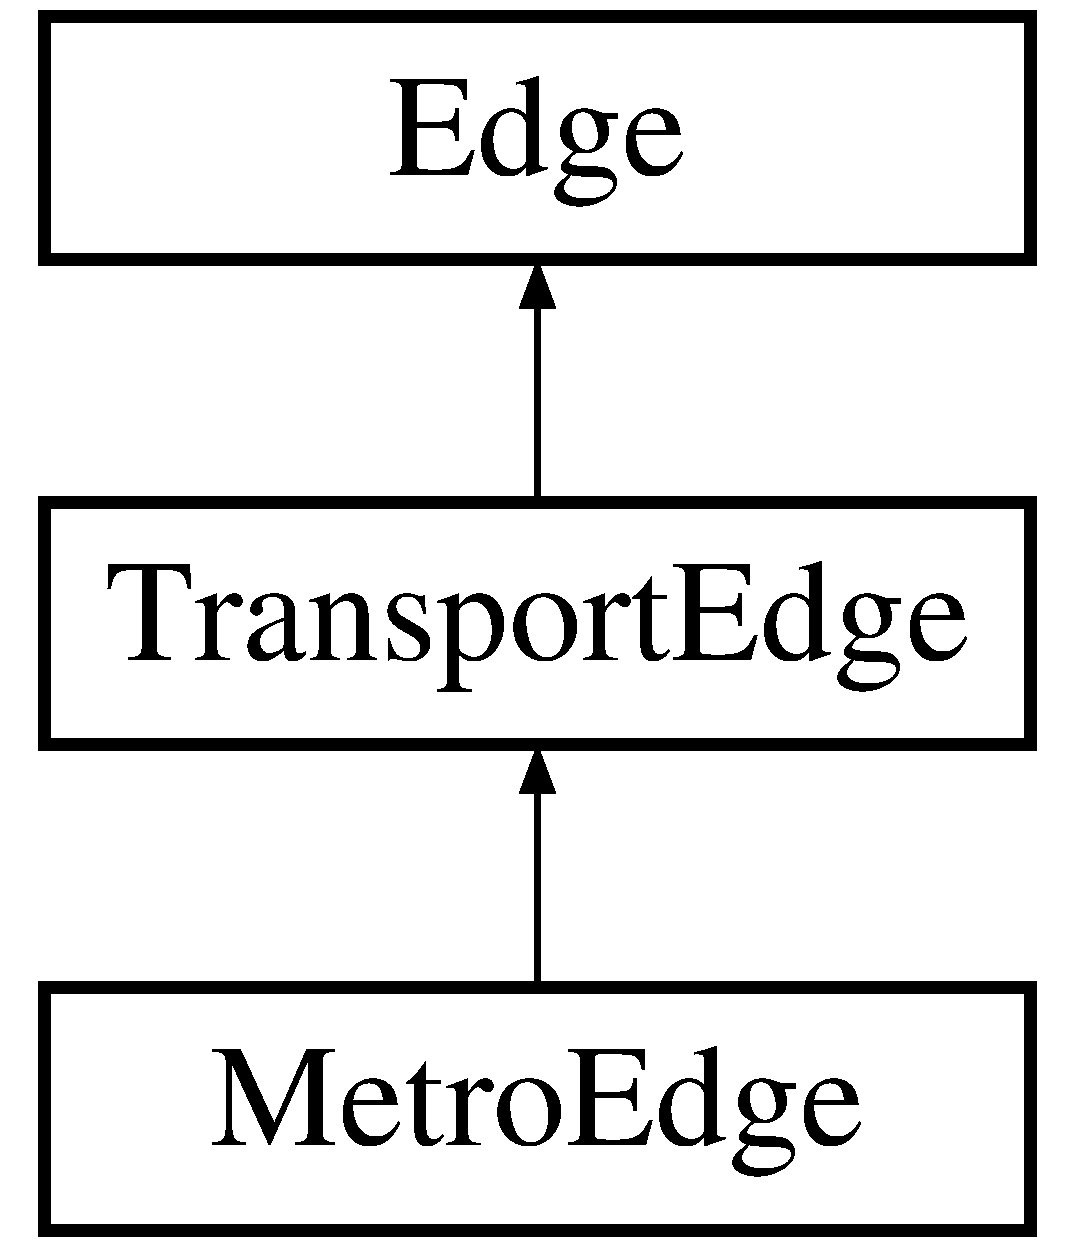
\includegraphics[height=3.000000cm]{class_metro_edge}
\end{center}
\end{figure}
\subsection*{Public Member Functions}
\begin{DoxyCompactItemize}
\item 
\hypertarget{class_metro_edge_acebfc5acd956610cf5dfd5c8dc3b645a}{}{\bfseries Metro\+Edge} (\hyperlink{class_vertex}{Vertex} $\ast$src, \hyperlink{class_vertex}{Vertex} $\ast$dst)\label{class_metro_edge_acebfc5acd956610cf5dfd5c8dc3b645a}

\item 
\hypertarget{class_metro_edge_aebaa11e7a8370e6adc2c525d97c36a1f}{}{\bfseries Metro\+Edge} (\hyperlink{class_vertex}{Vertex} $\ast$src, \hyperlink{class_vertex}{Vertex} $\ast$dst, const std\+::vector$<$ \hyperlink{class_coordinates}{Coordinates} $>$ \&line)\label{class_metro_edge_aebaa11e7a8370e6adc2c525d97c36a1f}

\item 
double \hyperlink{class_metro_edge_abe40bacd0e3d7e72fcdf7d0e38b2b311}{get\+Weight} ()
\begin{DoxyCompactList}\small\item\em calculates the edge\textquotesingle{}s weight (using Wight\+Info) \end{DoxyCompactList}\item 
double \hyperlink{class_metro_edge_a4cba8dae978df61bc931879b7ef2d528}{get\+Speed} () const 
\begin{DoxyCompactList}\small\item\em calculates the speed of the edge\textquotesingle{}s transport \end{DoxyCompactList}\end{DoxyCompactItemize}
\subsection*{Additional Inherited Members}


\subsection{Detailed Description}
Connection between two metro stops. 

\subsection{Member Function Documentation}
\hypertarget{class_metro_edge_a4cba8dae978df61bc931879b7ef2d528}{}\index{Metro\+Edge@{Metro\+Edge}!get\+Speed@{get\+Speed}}
\index{get\+Speed@{get\+Speed}!Metro\+Edge@{Metro\+Edge}}
\subsubsection[{get\+Speed}]{\setlength{\rightskip}{0pt plus 5cm}double Metro\+Edge\+::get\+Speed (
\begin{DoxyParamCaption}
{}
\end{DoxyParamCaption}
) const\hspace{0.3cm}{\ttfamily [virtual]}}\label{class_metro_edge_a4cba8dae978df61bc931879b7ef2d528}


calculates the speed of the edge\textquotesingle{}s transport 

\begin{DoxyReturn}{Returns}
speed of the transport 
\end{DoxyReturn}


Reimplemented from \hyperlink{class_transport_edge_a1e85cb198714507e2b1466b86f97b676}{Transport\+Edge}.

\hypertarget{class_metro_edge_abe40bacd0e3d7e72fcdf7d0e38b2b311}{}\index{Metro\+Edge@{Metro\+Edge}!get\+Weight@{get\+Weight}}
\index{get\+Weight@{get\+Weight}!Metro\+Edge@{Metro\+Edge}}
\subsubsection[{get\+Weight}]{\setlength{\rightskip}{0pt plus 5cm}double Metro\+Edge\+::get\+Weight (
\begin{DoxyParamCaption}
{}
\end{DoxyParamCaption}
)\hspace{0.3cm}{\ttfamily [virtual]}}\label{class_metro_edge_abe40bacd0e3d7e72fcdf7d0e38b2b311}


calculates the edge\textquotesingle{}s weight (using Wight\+Info) 

\begin{DoxyReturn}{Returns}
edge\textquotesingle{}s weighted cost 
\end{DoxyReturn}


Reimplemented from \hyperlink{class_transport_edge_ad2b8f66adec9223e97752ae1fb621c0e}{Transport\+Edge}.



The documentation for this class was generated from the following files\+:\begin{DoxyCompactItemize}
\item 
C\+:/\+Users/\+André/\+Desktop/test/transport/Metro\+Edge.\+h\item 
C\+:/\+Users/\+André/\+Desktop/test/transport/Metro\+Edge.\+cpp\end{DoxyCompactItemize}

\hypertarget{class_metro_route}{}\section{Metro\+Route Class Reference}
\label{class_metro_route}\index{Metro\+Route@{Metro\+Route}}


Represents a Metro Route -\/ set of metro stops ordered in a certain way.  




{\ttfamily \#include $<$Metro\+Route.\+h$>$}

Inheritance diagram for Metro\+Route\+:\begin{figure}[H]
\begin{center}
\leavevmode
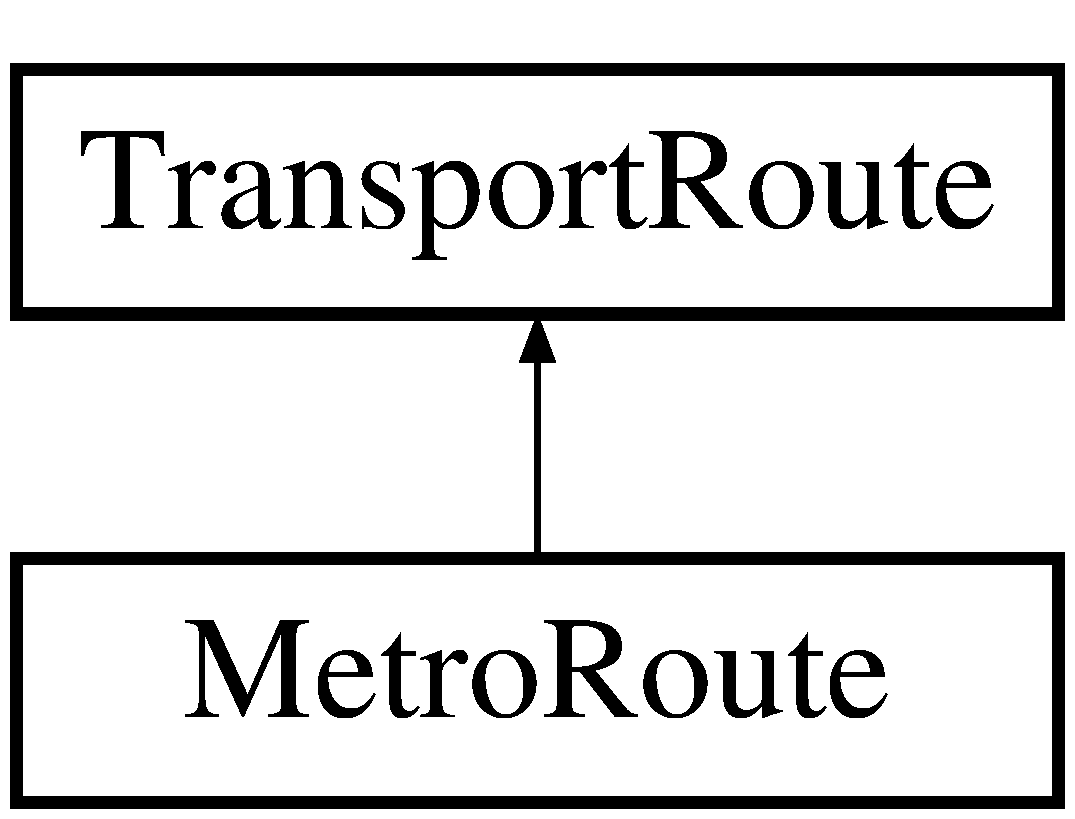
\includegraphics[height=2.000000cm]{class_metro_route}
\end{center}
\end{figure}
\subsection*{Public Member Functions}
\begin{DoxyCompactItemize}
\item 
\hyperlink{class_metro_route_aeb6e7b46697d63fd8373ca92a6ba9290}{Metro\+Route} (const std\+::string code, bool direction)
\begin{DoxyCompactList}\small\item\em class constructor \end{DoxyCompactList}\item 
\hypertarget{class_metro_route_a2445c22d84f3c3a2a6ccf65140b6b88d}{}double \hyperlink{class_metro_route_a2445c22d84f3c3a2a6ccf65140b6b88d}{get\+Speed} () const \label{class_metro_route_a2445c22d84f3c3a2a6ccf65140b6b88d}

\begin{DoxyCompactList}\small\item\em returns the Metro\textquotesingle{}s speed \end{DoxyCompactList}\item 
\hypertarget{class_metro_route_ae9c460e869b09a5a46abae9e3491978c}{}virtual \hyperlink{class_metro_route_ae9c460e869b09a5a46abae9e3491978c}{$\sim$\+Metro\+Route} ()\label{class_metro_route_ae9c460e869b09a5a46abae9e3491978c}

\begin{DoxyCompactList}\small\item\em class destructor \end{DoxyCompactList}\end{DoxyCompactItemize}
\subsection*{Additional Inherited Members}


\subsection{Detailed Description}
Represents a Metro Route -\/ set of metro stops ordered in a certain way. 

\subsection{Constructor \& Destructor Documentation}
\hypertarget{class_metro_route_aeb6e7b46697d63fd8373ca92a6ba9290}{}\index{Metro\+Route@{Metro\+Route}!Metro\+Route@{Metro\+Route}}
\index{Metro\+Route@{Metro\+Route}!Metro\+Route@{Metro\+Route}}
\subsubsection[{Metro\+Route}]{\setlength{\rightskip}{0pt plus 5cm}Metro\+Route\+::\+Metro\+Route (
\begin{DoxyParamCaption}
\item[{const std\+::string}]{code, }
\item[{bool}]{direction}
\end{DoxyParamCaption}
)}\label{class_metro_route_aeb6e7b46697d63fd8373ca92a6ba9290}


class constructor 


\begin{DoxyParams}{Parameters}
{\em code} & Route\textquotesingle{}s code \\
\hline
{\em directior} & specifies the direction of the route (true and false are opposite route directions, for the same route) \\
\hline
\end{DoxyParams}


The documentation for this class was generated from the following files\+:\begin{DoxyCompactItemize}
\item 
C\+:/\+Users/\+André/\+Desktop/test/transport/Metro\+Route.\+h\item 
C\+:/\+Users/\+André/\+Desktop/test/transport/Metro\+Route.\+cpp\end{DoxyCompactItemize}

\hypertarget{class_metro_stop}{}\section{Metro\+Stop Class Reference}
\label{class_metro_stop}\index{Metro\+Stop@{Metro\+Stop}}


Represents a Metro Stop.  




{\ttfamily \#include $<$Metro\+Stop.\+h$>$}

Inheritance diagram for Metro\+Stop\+:\begin{figure}[H]
\begin{center}
\leavevmode
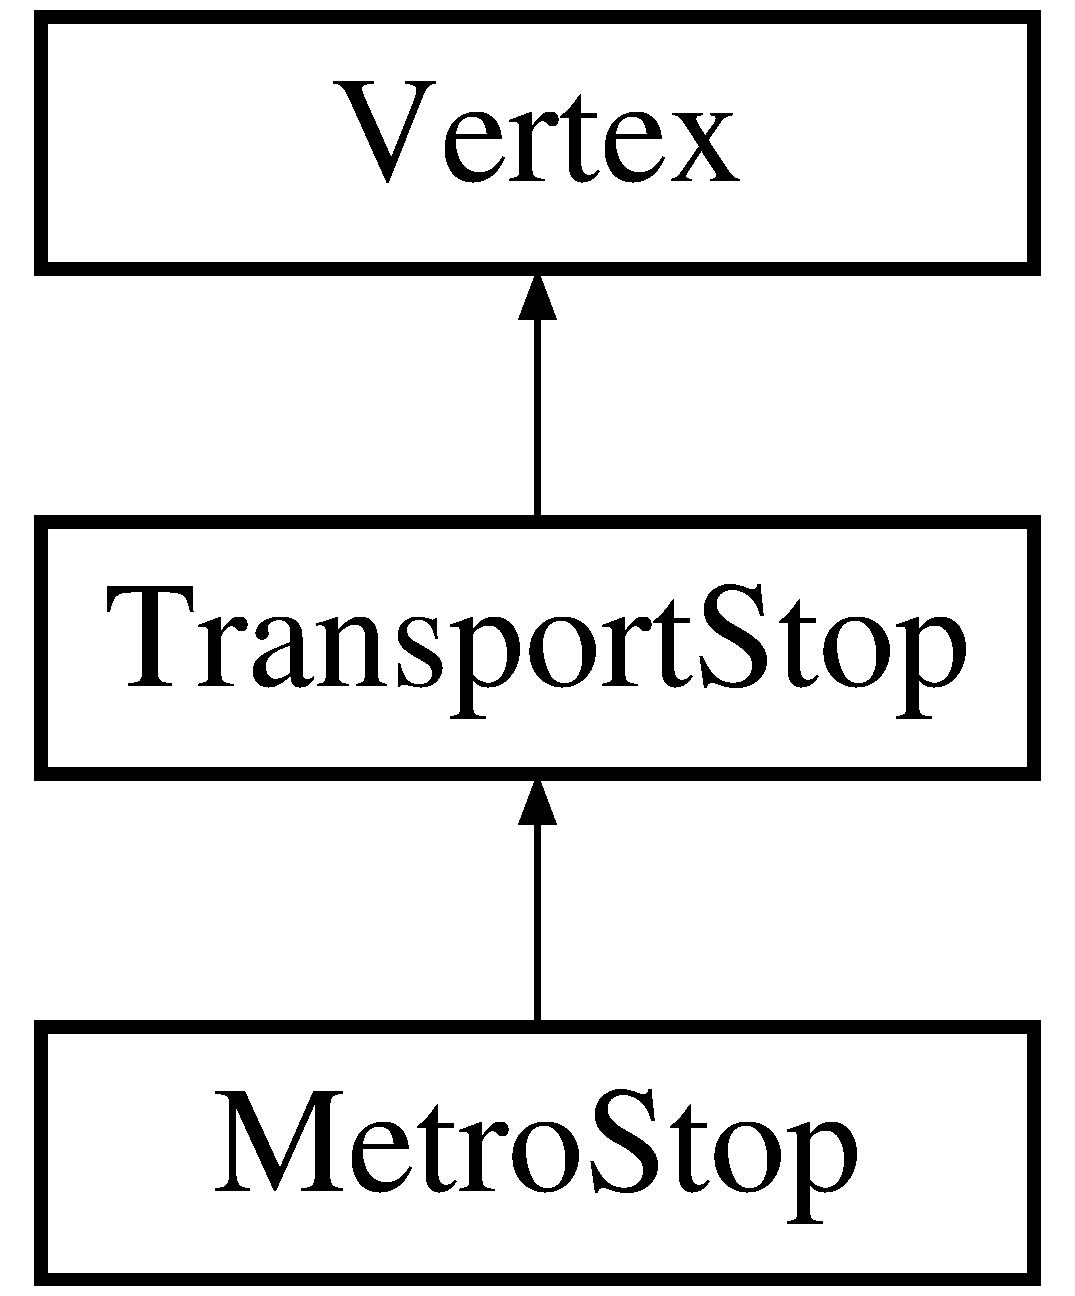
\includegraphics[height=3.000000cm]{class_metro_stop}
\end{center}
\end{figure}
\subsection*{Public Member Functions}
\begin{DoxyCompactItemize}
\item 
\hyperlink{class_metro_stop_a704608563c82fbd737f03df09f9b5fa9}{Metro\+Stop} (const std\+::string name, const \hyperlink{class_coordinates}{Coordinates} \&coords, const std\+::string \&route\+\_\+name)
\begin{DoxyCompactList}\small\item\em class constructor \end{DoxyCompactList}\item 
virtual std\+::string \hyperlink{class_metro_stop_ab2805dfc9f452e981ca71028c64cef38}{get\+Name\+And\+Type} () const 
\begin{DoxyCompactList}\small\item\em returns the stop\textquotesingle{}s name and type (e.\+x. Metro\+: I\+P\+O) \end{DoxyCompactList}\end{DoxyCompactItemize}
\subsection*{Static Public Attributes}
\begin{DoxyCompactItemize}
\item 
\hypertarget{class_metro_stop_a1d90f089b3625a13fce91942cdc99d50}{}static const double {\bfseries speed} = 1\label{class_metro_stop_a1d90f089b3625a13fce91942cdc99d50}

\end{DoxyCompactItemize}
\subsection*{Additional Inherited Members}


\subsection{Detailed Description}
Represents a Metro Stop. 

\subsection{Constructor \& Destructor Documentation}
\hypertarget{class_metro_stop_a704608563c82fbd737f03df09f9b5fa9}{}\index{Metro\+Stop@{Metro\+Stop}!Metro\+Stop@{Metro\+Stop}}
\index{Metro\+Stop@{Metro\+Stop}!Metro\+Stop@{Metro\+Stop}}
\subsubsection[{Metro\+Stop}]{\setlength{\rightskip}{0pt plus 5cm}Metro\+Stop\+::\+Metro\+Stop (
\begin{DoxyParamCaption}
\item[{const std\+::string}]{name, }
\item[{const {\bf Coordinates} \&}]{coords, }
\item[{const std\+::string \&}]{route\+\_\+name}
\end{DoxyParamCaption}
)}\label{class_metro_stop_a704608563c82fbd737f03df09f9b5fa9}


class constructor 


\begin{DoxyParams}{Parameters}
{\em name} & Stop\textquotesingle{}s name \\
\hline
{\em coords} & \hyperlink{class_coordinates}{Coordinates} of the Stop \\
\hline
\end{DoxyParams}


\subsection{Member Function Documentation}
\hypertarget{class_metro_stop_ab2805dfc9f452e981ca71028c64cef38}{}\index{Metro\+Stop@{Metro\+Stop}!get\+Name\+And\+Type@{get\+Name\+And\+Type}}
\index{get\+Name\+And\+Type@{get\+Name\+And\+Type}!Metro\+Stop@{Metro\+Stop}}
\subsubsection[{get\+Name\+And\+Type}]{\setlength{\rightskip}{0pt plus 5cm}virtual std\+::string Metro\+Stop\+::get\+Name\+And\+Type (
\begin{DoxyParamCaption}
{}
\end{DoxyParamCaption}
) const\hspace{0.3cm}{\ttfamily [inline]}, {\ttfamily [virtual]}}\label{class_metro_stop_ab2805dfc9f452e981ca71028c64cef38}


returns the stop\textquotesingle{}s name and type (e.\+x. Metro\+: I\+P\+O) 

\begin{DoxyReturn}{Returns}
string with stop name and type 
\end{DoxyReturn}


Reimplemented from \hyperlink{class_transport_stop_a245cff19d0ef473d56b93036042478ef}{Transport\+Stop}.



The documentation for this class was generated from the following files\+:\begin{DoxyCompactItemize}
\item 
C\+:/\+Users/\+André/\+Desktop/test/transport/Metro\+Stop.\+h\item 
C\+:/\+Users/\+André/\+Desktop/test/transport/Metro\+Stop.\+cpp\end{DoxyCompactItemize}

\hypertarget{class_path}{}\section{Path Class Reference}
\label{class_path}\index{Path@{Path}}


A set of edges representing a path between two points.  




{\ttfamily \#include $<$Path.\+h$>$}

\subsection*{Public Member Functions}
\begin{DoxyCompactItemize}
\item 
\hyperlink{class_path_ad2c6ad256aaa8f14e04a454e5690c961}{Path} (double cost)
\begin{DoxyCompactList}\small\item\em constructor for path \end{DoxyCompactList}\item 
vector$<$ \hyperlink{class_edge}{Edge} $\ast$ $>$ \hyperlink{class_path_a71778fdc2ff927535b0701d9064f7648}{get\+Edges} () const 
\begin{DoxyCompactList}\small\item\em get edges that form this path \end{DoxyCompactList}\item 
void \hyperlink{class_path_a3422b044fb9e5a713949278627ee1a9e}{add\+Edge\+End} (\hyperlink{class_edge}{Edge} $\ast$e)
\begin{DoxyCompactList}\small\item\em add edge to end of path \end{DoxyCompactList}\item 
void \hyperlink{class_path_a21f45a6d06681e5dc1b55f70bfdb877e}{add\+Edge\+Beginning} (\hyperlink{class_edge}{Edge} $\ast$e)
\begin{DoxyCompactList}\small\item\em add edge to beginning of path \end{DoxyCompactList}\item 
bool \hyperlink{class_path_ab1a846eee63b13e03724965d12d0a501}{operator==} (const \hyperlink{class_path}{Path} p2) const 
\begin{DoxyCompactList}\small\item\em equalitycomparison for paths \end{DoxyCompactList}\item 
\hypertarget{class_path_a8db20815826ef0f30515cb9e5c415da4}{}void \hyperlink{class_path_a8db20815826ef0f30515cb9e5c415da4}{remove\+Edge\+End} ()\label{class_path_a8db20815826ef0f30515cb9e5c415da4}

\begin{DoxyCompactList}\small\item\em remove the last edge from the path \end{DoxyCompactList}\item 
double \hyperlink{class_path_a2e92339063f0a7df0db8043828864c6d}{get\+Cost} () const 
\begin{DoxyCompactList}\small\item\em get the total weight of the path, assuming the it was correctly set \end{DoxyCompactList}\item 
void \hyperlink{class_path_a3b5228a0e1d37ca0293e82e32ba0fcce}{set\+Cost} (double cost)
\begin{DoxyCompactList}\small\item\em set the total weight of the path \end{DoxyCompactList}\item 
\hyperlink{class_path}{Path} \& \hyperlink{class_path_ad99e1ee379832d5ddb7f94c28759e771}{operator=} (const \hyperlink{class_path}{Path} \&p)
\begin{DoxyCompactList}\small\item\em set this path to be equal to another \end{DoxyCompactList}\end{DoxyCompactItemize}
\subsection*{Friends}
\begin{DoxyCompactItemize}
\item 
ostream \& \hyperlink{class_path_a46ad3a4bc74d84677e6c41299334a15e}{operator$<$$<$} (ostream \&os, \hyperlink{class_path}{Path} \&p)
\begin{DoxyCompactList}\small\item\em write path to outputstream \end{DoxyCompactList}\end{DoxyCompactItemize}


\subsection{Detailed Description}
A set of edges representing a path between two points. 

\subsection{Constructor \& Destructor Documentation}
\hypertarget{class_path_ad2c6ad256aaa8f14e04a454e5690c961}{}\index{Path@{Path}!Path@{Path}}
\index{Path@{Path}!Path@{Path}}
\subsubsection[{Path}]{\setlength{\rightskip}{0pt plus 5cm}Path\+::\+Path (
\begin{DoxyParamCaption}
\item[{double}]{cost}
\end{DoxyParamCaption}
)\hspace{0.3cm}{\ttfamily [inline]}}\label{class_path_ad2c6ad256aaa8f14e04a454e5690c961}


constructor for path 


\begin{DoxyParams}{Parameters}
{\em cost} & initial cost of path \\
\hline
\end{DoxyParams}


\subsection{Member Function Documentation}
\hypertarget{class_path_a21f45a6d06681e5dc1b55f70bfdb877e}{}\index{Path@{Path}!add\+Edge\+Beginning@{add\+Edge\+Beginning}}
\index{add\+Edge\+Beginning@{add\+Edge\+Beginning}!Path@{Path}}
\subsubsection[{add\+Edge\+Beginning}]{\setlength{\rightskip}{0pt plus 5cm}void Path\+::add\+Edge\+Beginning (
\begin{DoxyParamCaption}
\item[{{\bf Edge} $\ast$}]{e}
\end{DoxyParamCaption}
)\hspace{0.3cm}{\ttfamily [inline]}}\label{class_path_a21f45a6d06681e5dc1b55f70bfdb877e}


add edge to beginning of path 


\begin{DoxyParams}{Parameters}
{\em e} & new edge to add \\
\hline
\end{DoxyParams}
\hypertarget{class_path_a3422b044fb9e5a713949278627ee1a9e}{}\index{Path@{Path}!add\+Edge\+End@{add\+Edge\+End}}
\index{add\+Edge\+End@{add\+Edge\+End}!Path@{Path}}
\subsubsection[{add\+Edge\+End}]{\setlength{\rightskip}{0pt plus 5cm}void Path\+::add\+Edge\+End (
\begin{DoxyParamCaption}
\item[{{\bf Edge} $\ast$}]{e}
\end{DoxyParamCaption}
)\hspace{0.3cm}{\ttfamily [inline]}}\label{class_path_a3422b044fb9e5a713949278627ee1a9e}


add edge to end of path 


\begin{DoxyParams}{Parameters}
{\em e} & new edge to add \\
\hline
\end{DoxyParams}
\hypertarget{class_path_a2e92339063f0a7df0db8043828864c6d}{}\index{Path@{Path}!get\+Cost@{get\+Cost}}
\index{get\+Cost@{get\+Cost}!Path@{Path}}
\subsubsection[{get\+Cost}]{\setlength{\rightskip}{0pt plus 5cm}double Path\+::get\+Cost (
\begin{DoxyParamCaption}
{}
\end{DoxyParamCaption}
) const\hspace{0.3cm}{\ttfamily [inline]}}\label{class_path_a2e92339063f0a7df0db8043828864c6d}


get the total weight of the path, assuming the it was correctly set 

\begin{DoxyReturn}{Returns}
total cost of path 
\end{DoxyReturn}
\hypertarget{class_path_a71778fdc2ff927535b0701d9064f7648}{}\index{Path@{Path}!get\+Edges@{get\+Edges}}
\index{get\+Edges@{get\+Edges}!Path@{Path}}
\subsubsection[{get\+Edges}]{\setlength{\rightskip}{0pt plus 5cm}vector$<${\bf Edge}$\ast$$>$ Path\+::get\+Edges (
\begin{DoxyParamCaption}
{}
\end{DoxyParamCaption}
) const\hspace{0.3cm}{\ttfamily [inline]}}\label{class_path_a71778fdc2ff927535b0701d9064f7648}


get edges that form this path 

\begin{DoxyReturn}{Returns}
edges of path 
\end{DoxyReturn}
\hypertarget{class_path_ad99e1ee379832d5ddb7f94c28759e771}{}\index{Path@{Path}!operator=@{operator=}}
\index{operator=@{operator=}!Path@{Path}}
\subsubsection[{operator=}]{\setlength{\rightskip}{0pt plus 5cm}{\bf Path}\& Path\+::operator= (
\begin{DoxyParamCaption}
\item[{const {\bf Path} \&}]{p}
\end{DoxyParamCaption}
)\hspace{0.3cm}{\ttfamily [inline]}}\label{class_path_ad99e1ee379832d5ddb7f94c28759e771}


set this path to be equal to another 


\begin{DoxyParams}{Parameters}
{\em p} & path \\
\hline
\end{DoxyParams}
\begin{DoxyReturn}{Returns}
this path 
\end{DoxyReturn}
\hypertarget{class_path_ab1a846eee63b13e03724965d12d0a501}{}\index{Path@{Path}!operator==@{operator==}}
\index{operator==@{operator==}!Path@{Path}}
\subsubsection[{operator==}]{\setlength{\rightskip}{0pt plus 5cm}bool Path\+::operator== (
\begin{DoxyParamCaption}
\item[{const {\bf Path}}]{p2}
\end{DoxyParamCaption}
) const\hspace{0.3cm}{\ttfamily [inline]}}\label{class_path_ab1a846eee63b13e03724965d12d0a501}


equalitycomparison for paths 


\begin{DoxyParams}{Parameters}
{\em p2} & path to check for equality \\
\hline
\end{DoxyParams}
\begin{DoxyReturn}{Returns}
true if paths are equal 
\end{DoxyReturn}
\hypertarget{class_path_a3b5228a0e1d37ca0293e82e32ba0fcce}{}\index{Path@{Path}!set\+Cost@{set\+Cost}}
\index{set\+Cost@{set\+Cost}!Path@{Path}}
\subsubsection[{set\+Cost}]{\setlength{\rightskip}{0pt plus 5cm}void Path\+::set\+Cost (
\begin{DoxyParamCaption}
\item[{double}]{cost}
\end{DoxyParamCaption}
)\hspace{0.3cm}{\ttfamily [inline]}}\label{class_path_a3b5228a0e1d37ca0293e82e32ba0fcce}


set the total weight of the path 


\begin{DoxyParams}{Parameters}
{\em cost} & new cost of path \\
\hline
\end{DoxyParams}


\subsection{Friends And Related Function Documentation}
\hypertarget{class_path_a46ad3a4bc74d84677e6c41299334a15e}{}\index{Path@{Path}!operator$<$$<$@{operator$<$$<$}}
\index{operator$<$$<$@{operator$<$$<$}!Path@{Path}}
\subsubsection[{operator$<$$<$}]{\setlength{\rightskip}{0pt plus 5cm}ostream\& operator$<$$<$ (
\begin{DoxyParamCaption}
\item[{ostream \&}]{os, }
\item[{{\bf Path} \&}]{p}
\end{DoxyParamCaption}
)\hspace{0.3cm}{\ttfamily [friend]}}\label{class_path_a46ad3a4bc74d84677e6c41299334a15e}


write path to outputstream 


\begin{DoxyParams}{Parameters}
{\em os} & outputstream \\
\hline
{\em p} & path to write \\
\hline
\end{DoxyParams}
\begin{DoxyReturn}{Returns}
used outputstream 
\end{DoxyReturn}


The documentation for this class was generated from the following file\+:\begin{DoxyCompactItemize}
\item 
C\+:/\+Users/\+André/\+Desktop/test/graph/Path.\+h\end{DoxyCompactItemize}

\hypertarget{class_path_finder}{}\section{Path\+Finder Class Reference}
\label{class_path_finder}\index{Path\+Finder@{Path\+Finder}}


Interface to read user configurations and select algorithms and data structures to use.  




{\ttfamily \#include $<$Path\+Finder.\+h$>$}

\subsection*{Static Public Member Functions}
\begin{DoxyCompactItemize}
\item 
static \hyperlink{class_path}{Path} $\ast$ \hyperlink{class_path_finder_a7dcc8ea6a25e5ac9e42a94cb76340467}{find\+\_\+path} (\hyperlink{class_graph}{Graph} $\ast$g, \hyperlink{class_vertex}{Vertex} $\ast$ini, \hyperlink{class_vertex}{Vertex} $\ast$f, \hyperlink{class_program_config}{Program\+Config} conf)
\begin{DoxyCompactList}\small\item\em search for lowest cost path in graph from one vertex to another using the specified data structure and specified algorithm \end{DoxyCompactList}\end{DoxyCompactItemize}


\subsection{Detailed Description}
Interface to read user configurations and select algorithms and data structures to use. 

\subsection{Member Function Documentation}
\hypertarget{class_path_finder_a7dcc8ea6a25e5ac9e42a94cb76340467}{}\index{Path\+Finder@{Path\+Finder}!find\+\_\+path@{find\+\_\+path}}
\index{find\+\_\+path@{find\+\_\+path}!Path\+Finder@{Path\+Finder}}
\subsubsection[{find\+\_\+path}]{\setlength{\rightskip}{0pt plus 5cm}{\bf Path} $\ast$ Path\+Finder\+::find\+\_\+path (
\begin{DoxyParamCaption}
\item[{{\bf Graph} $\ast$}]{g, }
\item[{{\bf Vertex} $\ast$}]{ini, }
\item[{{\bf Vertex} $\ast$}]{f, }
\item[{{\bf Program\+Config}}]{conf}
\end{DoxyParamCaption}
)\hspace{0.3cm}{\ttfamily [static]}}\label{class_path_finder_a7dcc8ea6a25e5ac9e42a94cb76340467}


search for lowest cost path in graph from one vertex to another using the specified data structure and specified algorithm 


\begin{DoxyParams}{Parameters}
{\em g} & graph on which to perform search \\
\hline
{\em ini} & initial vertex \\
\hline
{\em f} & goal vertex \\
\hline
{\em conf} & configuration of program specifying chosen options \\
\hline
\end{DoxyParams}
\begin{DoxyReturn}{Returns}
path from initial vertex to goal of lowest cost, if there is none, the path will have no edges 
\end{DoxyReturn}


The documentation for this class was generated from the following files\+:\begin{DoxyCompactItemize}
\item 
C\+:/\+Users/\+André/\+Desktop/test/algorithms/Path\+Finder.\+h\item 
C\+:/\+Users/\+André/\+Desktop/test/algorithms/Path\+Finder.\+cpp\end{DoxyCompactItemize}

\hypertarget{class_program_config}{}\section{Program\+Config Class Reference}
\label{class_program_config}\index{Program\+Config@{Program\+Config}}


Stores the user configurations for the program\textquotesingle{}s execution.  




{\ttfamily \#include $<$Program\+Config.\+h$>$}

\subsection*{Public Member Functions}
\begin{DoxyCompactItemize}
\item 
\hypertarget{class_program_config_a518cb5f9a8c0a7470ea51b218cb9e2f3}{}bool {\bfseries wants\+Algorithm\+Performance} ()\label{class_program_config_a518cb5f9a8c0a7470ea51b218cb9e2f3}

\item 
\hypertarget{class_program_config_ae95569a91e2202d5ab11695af1a57620}{}Algorithm {\bfseries desired\+Algorithm} ()\label{class_program_config_ae95569a91e2202d5ab11695af1a57620}

\item 
\hypertarget{class_program_config_ae4d324614f4ce6918689c2d9bedb4548}{}Data\+Structure {\bfseries desired\+Data\+Structure} ()\label{class_program_config_ae4d324614f4ce6918689c2d9bedb4548}

\item 
\hypertarget{class_program_config_a5294986dc3d06899c9e75167e8296e83}{}Running\+Mode {\bfseries running\+Mode} ()\label{class_program_config_a5294986dc3d06899c9e75167e8296e83}

\item 
\hypertarget{class_program_config_a785a49f77c7eff93c43a82d1cac4973d}{}\hyperlink{class_hour}{Hour} {\bfseries get\+Start\+Hour} ()\label{class_program_config_a785a49f77c7eff93c43a82d1cac4973d}

\item 
\hypertarget{class_program_config_a6f2ba674157caea3c2d9bc20f1d6b46d}{}void {\bfseries set\+Wants\+Algorithm\+Performance} (bool wants)\label{class_program_config_a6f2ba674157caea3c2d9bc20f1d6b46d}

\item 
\hypertarget{class_program_config_a51efcb092f033936a1529f6903412bba}{}void {\bfseries set\+Algorithm} (Algorithm algorithm)\label{class_program_config_a51efcb092f033936a1529f6903412bba}

\item 
\hypertarget{class_program_config_a03787f2856673d700a5d04a9c7bb194e}{}void {\bfseries set\+Data\+Structure} (Data\+Structure data\+Structure)\label{class_program_config_a03787f2856673d700a5d04a9c7bb194e}

\item 
\hypertarget{class_program_config_aea84cce034f1b30e3231254028f7dbfe}{}void {\bfseries set\+Running\+Mode} (Running\+Mode running\+Mode)\label{class_program_config_aea84cce034f1b30e3231254028f7dbfe}

\item 
\hypertarget{class_program_config_a36f7574c78063a11777bc65d7822b602}{}void {\bfseries set\+Start\+Hour} (\hyperlink{class_hour}{Hour} start)\label{class_program_config_a36f7574c78063a11777bc65d7822b602}

\item 
\hypertarget{class_program_config_a04c3f32f627abf6ba27be5281b8dad47}{}void {\bfseries get\+From\+Console} ()\label{class_program_config_a04c3f32f627abf6ba27be5281b8dad47}

\item 
\hypertarget{class_program_config_af244c6ad33a0ed742eab41ac68c4424a}{}bool {\bfseries upon\+Exit\+Action} ()\label{class_program_config_af244c6ad33a0ed742eab41ac68c4424a}

\end{DoxyCompactItemize}


\subsection{Detailed Description}
Stores the user configurations for the program\textquotesingle{}s execution. 

The documentation for this class was generated from the following files\+:\begin{DoxyCompactItemize}
\item 
C\+:/\+Users/\+André/\+Desktop/test/Program\+Config.\+h\item 
C\+:/\+Users/\+André/\+Desktop/test/Program\+Config.\+cpp\end{DoxyCompactItemize}

\hypertarget{class_s_d_l_graph_draw}{}\section{S\+D\+L\+Graph\+Draw Class Reference}
\label{class_s_d_l_graph_draw}\index{S\+D\+L\+Graph\+Draw@{S\+D\+L\+Graph\+Draw}}


Implements an interface to draw a graph using S\+D\+L.  




{\ttfamily \#include $<$S\+D\+L\+Graph\+Draw.\+h$>$}

\subsection*{Static Public Member Functions}
\begin{DoxyCompactItemize}
\item 
\hypertarget{class_s_d_l_graph_draw_ae56dbc9d582adecd6fd98fd8808885aa}{}static void {\bfseries set\+Res} (unsigned int h, unsigned int v)\label{class_s_d_l_graph_draw_ae56dbc9d582adecd6fd98fd8808885aa}

\item 
\hypertarget{class_s_d_l_graph_draw_a6a0b3dcf2f40921433bc75f607367490}{}static int {\bfseries get\+Draw\+X} (double longi)\label{class_s_d_l_graph_draw_a6a0b3dcf2f40921433bc75f607367490}

\item 
\hypertarget{class_s_d_l_graph_draw_ab9ea987f3e278b871cda4dd52c2ea895}{}static int {\bfseries get\+Draw\+Y} (double lat)\label{class_s_d_l_graph_draw_ab9ea987f3e278b871cda4dd52c2ea895}

\item 
\hypertarget{class_s_d_l_graph_draw_afafb91d2683ba268d0996d7083b655db}{}static void {\bfseries draw\+Edge} (S\+D\+L\+\_\+\+Renderer $\ast$renderer, \hyperlink{class_edge}{Edge} $\ast$e, \hyperlink{class_s_d_l_r_g_b}{S\+D\+L\+R\+G\+B} color)\label{class_s_d_l_graph_draw_afafb91d2683ba268d0996d7083b655db}

\item 
\hypertarget{class_s_d_l_graph_draw_a25159ed823e3ad2630453d6c13b51f33}{}static void {\bfseries draw\+Graph} (S\+D\+L\+\_\+\+Renderer $\ast$renderer, \hyperlink{class_graph}{Graph} $\ast$e)\label{class_s_d_l_graph_draw_a25159ed823e3ad2630453d6c13b51f33}

\item 
\hypertarget{class_s_d_l_graph_draw_af84f868a9558733840d64d82751bdd85}{}static void {\bfseries draw\+Path} (S\+D\+L\+\_\+\+Renderer $\ast$renderer, \hyperlink{class_path}{Path} $\ast$e)\label{class_s_d_l_graph_draw_af84f868a9558733840d64d82751bdd85}

\item 
\hypertarget{class_s_d_l_graph_draw_af9a230f883ac350775a38d0eee926556}{}static void {\bfseries draw\+Vertex} (S\+D\+L\+\_\+\+Renderer $\ast$renderer, \hyperlink{class_vertex}{Vertex} $\ast$v, int size, \hyperlink{class_s_d_l_r_g_b}{S\+D\+L\+R\+G\+B} color)\label{class_s_d_l_graph_draw_af9a230f883ac350775a38d0eee926556}

\item 
\hypertarget{class_s_d_l_graph_draw_aa9c19af048839c159e655a30c7a7c192}{}static void {\bfseries draw\+Edge} (S\+D\+L\+\_\+\+Renderer $\ast$renderer, \hyperlink{class_camera}{Camera} $\ast$c, \hyperlink{class_edge}{Edge} $\ast$e, \hyperlink{class_s_d_l_r_g_b}{S\+D\+L\+R\+G\+B} color)\label{class_s_d_l_graph_draw_aa9c19af048839c159e655a30c7a7c192}

\item 
\hypertarget{class_s_d_l_graph_draw_a4585253ab552da3e2c0d30a9cee26b25}{}static void {\bfseries draw\+Graph} (S\+D\+L\+\_\+\+Renderer $\ast$renderer, \hyperlink{class_camera}{Camera} $\ast$c, \hyperlink{class_graph}{Graph} $\ast$e)\label{class_s_d_l_graph_draw_a4585253ab552da3e2c0d30a9cee26b25}

\item 
\hypertarget{class_s_d_l_graph_draw_a1fedec02c2544aa6ac98f39912d068da}{}static void {\bfseries draw\+Path} (S\+D\+L\+\_\+\+Renderer $\ast$renderer, \hyperlink{class_camera}{Camera} $\ast$c, \hyperlink{class_path}{Path} $\ast$e, \hyperlink{class_s_d_l_r_g_b}{S\+D\+L\+R\+G\+B} color)\label{class_s_d_l_graph_draw_a1fedec02c2544aa6ac98f39912d068da}

\item 
\hypertarget{class_s_d_l_graph_draw_aa9606dc080a41bf5f135544f070a974a}{}static void {\bfseries draw\+Vertex} (S\+D\+L\+\_\+\+Renderer $\ast$renderer, \hyperlink{class_camera}{Camera} $\ast$c, \hyperlink{class_vertex}{Vertex} $\ast$v, int size, \hyperlink{class_s_d_l_r_g_b}{S\+D\+L\+R\+G\+B} color)\label{class_s_d_l_graph_draw_aa9606dc080a41bf5f135544f070a974a}

\item 
\hypertarget{class_s_d_l_graph_draw_a5204f8ce650f7acab334b4f38c8c13d0}{}static void {\bfseries draw\+Slider} (S\+D\+L\+\_\+\+Renderer $\ast$renderer, \hyperlink{class_slider}{Slider} $\ast$slider, \hyperlink{class_s_d_l_r_g_b}{S\+D\+L\+R\+G\+B} color1, \hyperlink{class_s_d_l_r_g_b}{S\+D\+L\+R\+G\+B} color2)\label{class_s_d_l_graph_draw_a5204f8ce650f7acab334b4f38c8c13d0}

\item 
\hypertarget{class_s_d_l_graph_draw_a4d8be1f34ec8eccb2e7e80d7228cf4b6}{}static unsigned int {\bfseries get\+H\+Res} ()\label{class_s_d_l_graph_draw_a4d8be1f34ec8eccb2e7e80d7228cf4b6}

\item 
\hypertarget{class_s_d_l_graph_draw_ae9350eadef9862b43aa9e6c5c5f87fb3}{}static unsigned int {\bfseries get\+V\+Res} ()\label{class_s_d_l_graph_draw_ae9350eadef9862b43aa9e6c5c5f87fb3}

\item 
\hypertarget{class_s_d_l_graph_draw_aeb392bdfcb20bc810b957078606785c7}{}static double {\bfseries get\+Maxlat} ()\label{class_s_d_l_graph_draw_aeb392bdfcb20bc810b957078606785c7}

\item 
\hypertarget{class_s_d_l_graph_draw_afc9db32ed6b0f8e4c4038b54c64ead17}{}static void {\bfseries set\+Maxlat} (double value)\label{class_s_d_l_graph_draw_afc9db32ed6b0f8e4c4038b54c64ead17}

\item 
\hypertarget{class_s_d_l_graph_draw_ada42c2cc2296ebb0a3aadd0251ad2ae1}{}static double {\bfseries get\+Maxlong} ()\label{class_s_d_l_graph_draw_ada42c2cc2296ebb0a3aadd0251ad2ae1}

\item 
\hypertarget{class_s_d_l_graph_draw_abc69645ab176b5641e86f381a01808f3}{}static void {\bfseries set\+Maxlong} (double value)\label{class_s_d_l_graph_draw_abc69645ab176b5641e86f381a01808f3}

\item 
\hypertarget{class_s_d_l_graph_draw_a04f1f6a61bdb041f1aac598c1cb07587}{}static double {\bfseries get\+Minlat} ()\label{class_s_d_l_graph_draw_a04f1f6a61bdb041f1aac598c1cb07587}

\item 
\hypertarget{class_s_d_l_graph_draw_aac068db479965497c6a3c4e0735f9980}{}static void {\bfseries set\+Minlat} (double value)\label{class_s_d_l_graph_draw_aac068db479965497c6a3c4e0735f9980}

\item 
\hypertarget{class_s_d_l_graph_draw_a7047fc03c8b1032b8f3a4fda05c483ae}{}static double {\bfseries get\+Minlong} ()\label{class_s_d_l_graph_draw_a7047fc03c8b1032b8f3a4fda05c483ae}

\item 
\hypertarget{class_s_d_l_graph_draw_a8af0e7e103ed4b2f4fbdddf77e90dc2c}{}static void {\bfseries set\+Minlong} (double value)\label{class_s_d_l_graph_draw_a8af0e7e103ed4b2f4fbdddf77e90dc2c}

\item 
\hypertarget{class_s_d_l_graph_draw_a8606399583858d969b2e0cd0b5e832ca}{}static void {\bfseries set\+Values} (double minx, double miny, double maxx, double maxy)\label{class_s_d_l_graph_draw_a8606399583858d969b2e0cd0b5e832ca}

\item 
\hypertarget{class_s_d_l_graph_draw_a825f75426a2b290bc511215e1a25dc2c}{}static void {\bfseries draw\+Map\+Edge} (S\+D\+L\+\_\+\+Renderer $\ast$renderer, \hyperlink{class_camera}{Camera} $\ast$c, \hyperlink{class_edge}{Edge} $\ast$e, bool debug)\label{class_s_d_l_graph_draw_a825f75426a2b290bc511215e1a25dc2c}

\item 
\hypertarget{class_s_d_l_graph_draw_a6cf3b33aa5828e7ef9f60925f9f915e9}{}static void {\bfseries draw\+Map\+Vertex} (S\+D\+L\+\_\+\+Renderer $\ast$renderer, \hyperlink{class_camera}{Camera} $\ast$c, \hyperlink{class_vertex}{Vertex} $\ast$e, \hyperlink{class_s_d_l_r_g_b}{S\+D\+L\+R\+G\+B} color)\label{class_s_d_l_graph_draw_a6cf3b33aa5828e7ef9f60925f9f915e9}

\item 
\hypertarget{class_s_d_l_graph_draw_aa15194fdd2703387939b859d6e6e30aa}{}static void {\bfseries draw\+Map\+Vertex\+Pos} (S\+D\+L\+\_\+\+Renderer $\ast$renderer, \hyperlink{class_camera}{Camera} $\ast$c, int renderx, int rendery, \hyperlink{class_s_d_l_r_g_b}{S\+D\+L\+R\+G\+B} color)\label{class_s_d_l_graph_draw_aa15194fdd2703387939b859d6e6e30aa}

\item 
\hypertarget{class_s_d_l_graph_draw_a6cf48dea85e7383cf40c532bc7bdeae1}{}static void {\bfseries draw\+Map\+Graph} (S\+D\+L\+\_\+\+Renderer $\ast$renderer, \hyperlink{class_camera}{Camera} $\ast$c, \hyperlink{class_graph}{Graph} $\ast$g, \hyperlink{class_vertex}{Vertex} $\ast$src, \hyperlink{class_vertex}{Vertex} $\ast$dst, \hyperlink{class_path}{Path} $\ast$p)\label{class_s_d_l_graph_draw_a6cf48dea85e7383cf40c532bc7bdeae1}

\item 
\hypertarget{class_s_d_l_graph_draw_ad220735800321912cb928b92d3cee3fb}{}static void {\bfseries draw\+Map\+Graph\+Performance} (S\+D\+L\+\_\+\+Renderer $\ast$renderer, \hyperlink{class_camera}{Camera} $\ast$c, \hyperlink{class_graph}{Graph} $\ast$g, \hyperlink{class_vertex}{Vertex} $\ast$src, \hyperlink{class_vertex}{Vertex} $\ast$dst, \hyperlink{class_path}{Path} $\ast$p)\label{class_s_d_l_graph_draw_ad220735800321912cb928b92d3cee3fb}

\end{DoxyCompactItemize}


\subsection{Detailed Description}
Implements an interface to draw a graph using S\+D\+L. 

The documentation for this class was generated from the following files\+:\begin{DoxyCompactItemize}
\item 
C\+:/\+Users/\+André/\+Desktop/test/gui/S\+D\+L\+Graph\+Draw.\+h\item 
C\+:/\+Users/\+André/\+Desktop/test/gui/S\+D\+L\+Graph\+Draw.\+cpp\end{DoxyCompactItemize}

\hypertarget{class_s_d_l_r_g_b}{}\section{S\+D\+L\+R\+G\+B Class Reference}
\label{class_s_d_l_r_g_b}\index{S\+D\+L\+R\+G\+B@{S\+D\+L\+R\+G\+B}}
\subsection*{Public Member Functions}
\begin{DoxyCompactItemize}
\item 
\hypertarget{class_s_d_l_r_g_b_ab1c9e2530d04232a85fe11e0419adc40}{}{\bfseries S\+D\+L\+R\+G\+B} (unsigned char red, unsigned char blue, unsigned char green)\label{class_s_d_l_r_g_b_ab1c9e2530d04232a85fe11e0419adc40}

\end{DoxyCompactItemize}
\subsection*{Public Attributes}
\begin{DoxyCompactItemize}
\item 
\hypertarget{class_s_d_l_r_g_b_ae89fec7cd2e6b0f3ca07d82cb530878f}{}unsigned char {\bfseries red}\label{class_s_d_l_r_g_b_ae89fec7cd2e6b0f3ca07d82cb530878f}

\item 
\hypertarget{class_s_d_l_r_g_b_adea42fe779da29234102660d5b340990}{}unsigned char {\bfseries blue}\label{class_s_d_l_r_g_b_adea42fe779da29234102660d5b340990}

\item 
\hypertarget{class_s_d_l_r_g_b_a84a775d2f8e889d051258c421b318f9b}{}unsigned char {\bfseries green}\label{class_s_d_l_r_g_b_a84a775d2f8e889d051258c421b318f9b}

\end{DoxyCompactItemize}


The documentation for this class was generated from the following file\+:\begin{DoxyCompactItemize}
\item 
C\+:/\+Users/\+André/\+Desktop/test/gui/S\+D\+L\+R\+G\+B.\+h\end{DoxyCompactItemize}

\hypertarget{class_slider}{}\section{Slider Class Reference}
\label{class_slider}\index{Slider@{Slider}}


A slider interface, with a bar able to slide over another, representing a value between two limits.  




{\ttfamily \#include $<$Slider.\+h$>$}

\subsection*{Public Member Functions}
\begin{DoxyCompactItemize}
\item 
\hypertarget{class_slider_ac456725827e4cdc35cb5d5c1e2662910}{}{\bfseries Slider} (int x, int y, int width, int height, int cursor\+Width, int cursor\+Height, double min, double max, double value, bool horizontal=true)\label{class_slider_ac456725827e4cdc35cb5d5c1e2662910}

\item 
\hypertarget{class_slider_a2909285efe7aa44f9ff1372fa679e842}{}bool {\bfseries set\+Value} (double value)\label{class_slider_a2909285efe7aa44f9ff1372fa679e842}

\item 
\hypertarget{class_slider_ace4fffe8ad4e2b2c4cd2cda06dedc848}{}double {\bfseries get\+Value} () const \label{class_slider_ace4fffe8ad4e2b2c4cd2cda06dedc848}

\item 
\hypertarget{class_slider_a579ee955a2b54659b00b1a42e32e3c66}{}int {\bfseries get\+Height} () const \label{class_slider_a579ee955a2b54659b00b1a42e32e3c66}

\item 
\hypertarget{class_slider_a670f1e9dd575682f3d41489ed11bfab6}{}void {\bfseries set\+Height} (int height)\label{class_slider_a670f1e9dd575682f3d41489ed11bfab6}

\item 
\hypertarget{class_slider_a5482e9d9ea595b16c9b47dc0dfe9145d}{}double {\bfseries get\+Max} () const \label{class_slider_a5482e9d9ea595b16c9b47dc0dfe9145d}

\item 
\hypertarget{class_slider_abcb2840e64fc0ff5efe25e54884aef2c}{}void {\bfseries set\+Max} (double max)\label{class_slider_abcb2840e64fc0ff5efe25e54884aef2c}

\item 
\hypertarget{class_slider_a1e896244a3456cd73ed6a15b099613c4}{}double {\bfseries get\+Min} () const \label{class_slider_a1e896244a3456cd73ed6a15b099613c4}

\item 
\hypertarget{class_slider_a3928cc8e14d3f0707721306893f6c838}{}void {\bfseries set\+Min} (double min)\label{class_slider_a3928cc8e14d3f0707721306893f6c838}

\item 
\hypertarget{class_slider_a7795bfcac92d4e15cbdc211f4491c326}{}int {\bfseries get\+Width} () const \label{class_slider_a7795bfcac92d4e15cbdc211f4491c326}

\item 
\hypertarget{class_slider_aa49137d24889b83a49b77bd060237278}{}void {\bfseries set\+Width} (int width)\label{class_slider_aa49137d24889b83a49b77bd060237278}

\item 
\hypertarget{class_slider_a7b088eb7c67e386db8b7a3ad60eccb6a}{}int {\bfseries get\+X} () const \label{class_slider_a7b088eb7c67e386db8b7a3ad60eccb6a}

\item 
\hypertarget{class_slider_a7d00227f6acc8326f845181ccfc7e0a2}{}void {\bfseries set\+X} (int x)\label{class_slider_a7d00227f6acc8326f845181ccfc7e0a2}

\item 
\hypertarget{class_slider_a8e193dacb39f493e9bd9f3527a36f0cc}{}int {\bfseries get\+Y} () const \label{class_slider_a8e193dacb39f493e9bd9f3527a36f0cc}

\item 
\hypertarget{class_slider_ae37e42aa2ac576b080b7258dbe418453}{}void {\bfseries set\+Y} (int y)\label{class_slider_ae37e42aa2ac576b080b7258dbe418453}

\item 
\hypertarget{class_slider_a83d87d20e8081183cfcb1e3280de05e4}{}bool {\bfseries is\+Horizontal} () const \label{class_slider_a83d87d20e8081183cfcb1e3280de05e4}

\item 
\hypertarget{class_slider_ac434719cecbc1ddc246f9f565b3bef29}{}void {\bfseries set\+Horizontal} (bool horizontal)\label{class_slider_ac434719cecbc1ddc246f9f565b3bef29}

\item 
\hypertarget{class_slider_a487abaeb6b222126010bd0bde03c19d3}{}bool {\bfseries set\+Value\+U\+I} (int screen\+Pos)\label{class_slider_a487abaeb6b222126010bd0bde03c19d3}

\item 
\hypertarget{class_slider_ad866de0efb61986a82bdb50512acff3c}{}double {\bfseries res\+To\+Value} (int res)\label{class_slider_ad866de0efb61986a82bdb50512acff3c}

\item 
\hypertarget{class_slider_a1dde4ef475c2dff3b5f6542bf1964867}{}int {\bfseries value\+To\+Res} (double value)\label{class_slider_a1dde4ef475c2dff3b5f6542bf1964867}

\item 
\hypertarget{class_slider_ada143a519b663770b66de77fc3ef857e}{}int {\bfseries get\+Cursor\+Height} () const \label{class_slider_ada143a519b663770b66de77fc3ef857e}

\item 
\hypertarget{class_slider_a8f4543769959217510a5ac1e8bfaa635}{}void {\bfseries set\+Cursor\+Height} (int cursor\+Height)\label{class_slider_a8f4543769959217510a5ac1e8bfaa635}

\item 
\hypertarget{class_slider_aa163928f61bc81520c0c7fd93afbf5d2}{}int {\bfseries get\+Cursor\+Width} () const \label{class_slider_aa163928f61bc81520c0c7fd93afbf5d2}

\item 
\hypertarget{class_slider_ac05a2d600978b4624bcf5d0a03e1d038}{}void {\bfseries set\+Cursor\+Width} (int cursor\+Width)\label{class_slider_ac05a2d600978b4624bcf5d0a03e1d038}

\item 
\hypertarget{class_slider_aa10105d4f3e2a2437ed1e02a6e658406}{}int {\bfseries get\+Cursor\+X} ()\label{class_slider_aa10105d4f3e2a2437ed1e02a6e658406}

\item 
\hypertarget{class_slider_a06b36fa75a35eaef9e1ae4c1c94f4648}{}int {\bfseries get\+Cursor\+Y} ()\label{class_slider_a06b36fa75a35eaef9e1ae4c1c94f4648}

\item 
\hypertarget{class_slider_a0224c749072fc2123f4fd41e08fcc06e}{}bool {\bfseries select} (int pos\+X, int pos\+Y)\label{class_slider_a0224c749072fc2123f4fd41e08fcc06e}

\item 
\hypertarget{class_slider_a4ddcc0bd4e801071f7b32f6612d59a23}{}bool {\bfseries is\+Selected} () const \label{class_slider_a4ddcc0bd4e801071f7b32f6612d59a23}

\item 
\hypertarget{class_slider_a82aeb84ffd329dc6148827c2418a8e87}{}void {\bfseries set\+Selected} (bool selected)\label{class_slider_a82aeb84ffd329dc6148827c2418a8e87}

\end{DoxyCompactItemize}


\subsection{Detailed Description}
A slider interface, with a bar able to slide over another, representing a value between two limits. 

The documentation for this class was generated from the following file\+:\begin{DoxyCompactItemize}
\item 
C\+:/\+Users/\+André/\+Desktop/test/gui/Slider.\+h\end{DoxyCompactItemize}

\hypertarget{class_transport_edge}{}\section{Transport\+Edge Class Reference}
\label{class_transport_edge}\index{Transport\+Edge@{Transport\+Edge}}


represents the connection between two stops  




{\ttfamily \#include $<$Transport\+Edge.\+h$>$}

Inheritance diagram for Transport\+Edge\+:\begin{figure}[H]
\begin{center}
\leavevmode
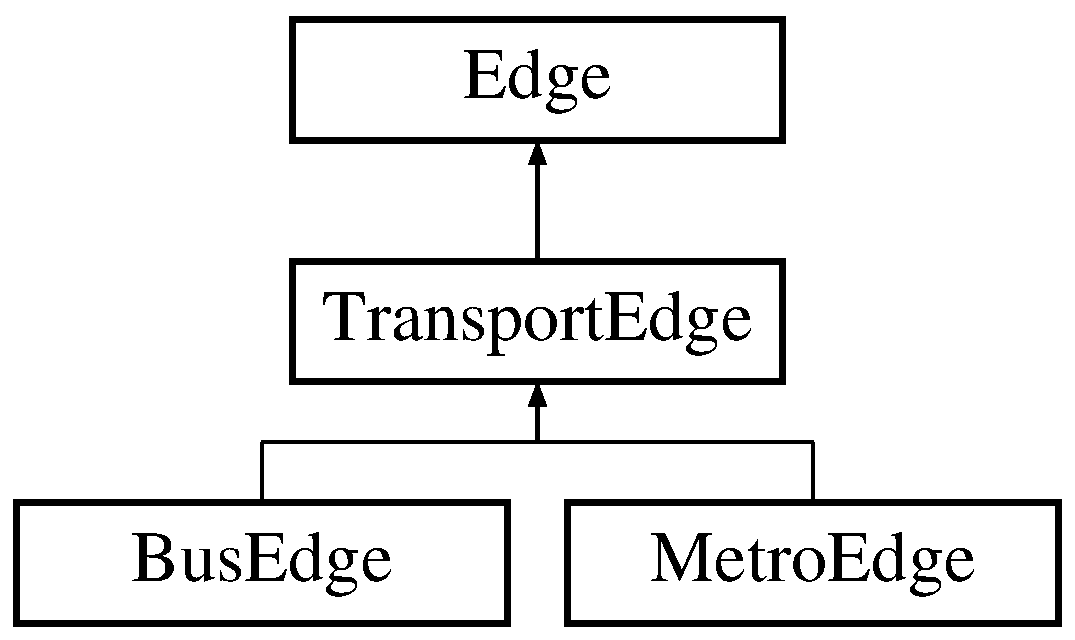
\includegraphics[height=3.000000cm]{class_transport_edge}
\end{center}
\end{figure}
\subsection*{Public Member Functions}
\begin{DoxyCompactItemize}
\item 
\hyperlink{class_transport_edge_a17138b409239b50080a9401bd1f5d55b}{Transport\+Edge} (\hyperlink{class_vertex}{Vertex} $\ast$src, \hyperlink{class_vertex}{Vertex} $\ast$dst)
\begin{DoxyCompactList}\small\item\em class constructor \end{DoxyCompactList}\item 
\hyperlink{class_transport_edge_a1b92b947e39bf283dfd9288559f44132}{Transport\+Edge} (\hyperlink{class_vertex}{Vertex} $\ast$src, \hyperlink{class_vertex}{Vertex} $\ast$dst, const vector$<$ \hyperlink{class_coordinates}{Coordinates} $>$ \&line)
\begin{DoxyCompactList}\small\item\em class constructor \end{DoxyCompactList}\item 
void \hyperlink{class_transport_edge_aa1da957ea215ff6ec5aa6dc8132eb381}{add\+Point} (const \hyperlink{class_coordinates}{Coordinates} \&coords)
\begin{DoxyCompactList}\small\item\em adds a geographical point to the edge\textquotesingle{}s set of points \end{DoxyCompactList}\item 
virtual double \hyperlink{class_transport_edge_ad2b8f66adec9223e97752ae1fb621c0e}{get\+Weight} ()
\begin{DoxyCompactList}\small\item\em calculates the edge\textquotesingle{}s weight (using Wight\+Info) \end{DoxyCompactList}\item 
\hyperlink{class_weight_info}{Weight\+Info} \hyperlink{class_transport_edge_a0087341702150f0cd7fe35c667222ee8}{get\+Weight\+Info} ()
\begin{DoxyCompactList}\small\item\em returns the \hyperlink{class_weight_info}{Weight\+Info} of the edge (thus separating the different weights of crossing the edge) \end{DoxyCompactList}\item 
const std\+::vector$<$ \hyperlink{class_coordinates}{Coordinates} $>$ \& \hyperlink{class_transport_edge_a9332ec7a11cd5d9b5f01df7422a8a178}{get\+Line} () const 
\begin{DoxyCompactList}\small\item\em returns the set of points that represent the edge \end{DoxyCompactList}\item 
virtual double \hyperlink{class_transport_edge_a1e85cb198714507e2b1466b86f97b676}{get\+Speed} () const 
\begin{DoxyCompactList}\small\item\em calculates the speed of the edge\textquotesingle{}s transport \end{DoxyCompactList}\item 
virtual double \hyperlink{class_transport_edge_ac9ece7be6c95ec5fa56cae347f2716dd}{calculate\+Time} () const 
\begin{DoxyCompactList}\small\item\em calculates the time it takes to cross the edge \end{DoxyCompactList}\item 
\hypertarget{class_transport_edge_a36780733e6cf6784e895e2562042abee}{}virtual \hyperlink{class_transport_edge_a36780733e6cf6784e895e2562042abee}{$\sim$\+Transport\+Edge} ()\label{class_transport_edge_a36780733e6cf6784e895e2562042abee}

\begin{DoxyCompactList}\small\item\em class destructor \end{DoxyCompactList}\item 
bool \hyperlink{class_transport_edge_ac1513075a93041cea50ea82927760bec}{get\+Visible} ()
\begin{DoxyCompactList}\small\item\em returns a boolean that represents wether the edge must be drawn or not \end{DoxyCompactList}\end{DoxyCompactItemize}
\subsection*{Protected Attributes}
\begin{DoxyCompactItemize}
\item 
\hypertarget{class_transport_edge_a907da2ef63c5d90cfe12a78b21e2292e}{}std\+::vector$<$ \hyperlink{class_coordinates}{Coordinates} $>$ {\bfseries line}\label{class_transport_edge_a907da2ef63c5d90cfe12a78b21e2292e}

\item 
\hypertarget{class_transport_edge_aac54ca3f2f4fc0248dc20efd93806f0c}{}\hyperlink{class_weight_info}{Weight\+Info} {\bfseries weight}\label{class_transport_edge_aac54ca3f2f4fc0248dc20efd93806f0c}

\item 
\hypertarget{class_transport_edge_a3f7f7bfb6bdcbca7ce1d58e5fe102e86}{}bool {\bfseries visible}\label{class_transport_edge_a3f7f7bfb6bdcbca7ce1d58e5fe102e86}

\end{DoxyCompactItemize}


\subsection{Detailed Description}
represents the connection between two stops 

\subsection{Constructor \& Destructor Documentation}
\hypertarget{class_transport_edge_a17138b409239b50080a9401bd1f5d55b}{}\index{Transport\+Edge@{Transport\+Edge}!Transport\+Edge@{Transport\+Edge}}
\index{Transport\+Edge@{Transport\+Edge}!Transport\+Edge@{Transport\+Edge}}
\subsubsection[{Transport\+Edge}]{\setlength{\rightskip}{0pt plus 5cm}Transport\+Edge\+::\+Transport\+Edge (
\begin{DoxyParamCaption}
\item[{{\bf Vertex} $\ast$}]{src, }
\item[{{\bf Vertex} $\ast$}]{dst}
\end{DoxyParamCaption}
)}\label{class_transport_edge_a17138b409239b50080a9401bd1f5d55b}


class constructor 


\begin{DoxyParams}{Parameters}
{\em src} & \hyperlink{class_edge}{Edge}\textquotesingle{}s source vertex \\
\hline
{\em dst} & \hyperlink{class_edge}{Edge}\textquotesingle{}s destination vertex \\
\hline
\end{DoxyParams}
\hypertarget{class_transport_edge_a1b92b947e39bf283dfd9288559f44132}{}\index{Transport\+Edge@{Transport\+Edge}!Transport\+Edge@{Transport\+Edge}}
\index{Transport\+Edge@{Transport\+Edge}!Transport\+Edge@{Transport\+Edge}}
\subsubsection[{Transport\+Edge}]{\setlength{\rightskip}{0pt plus 5cm}Transport\+Edge\+::\+Transport\+Edge (
\begin{DoxyParamCaption}
\item[{{\bf Vertex} $\ast$}]{src, }
\item[{{\bf Vertex} $\ast$}]{dst, }
\item[{const vector$<$ {\bf Coordinates} $>$ \&}]{line}
\end{DoxyParamCaption}
)}\label{class_transport_edge_a1b92b947e39bf283dfd9288559f44132}


class constructor 


\begin{DoxyParams}{Parameters}
{\em src} & \hyperlink{class_edge}{Edge}\textquotesingle{}s source vertex \\
\hline
{\em dst} & \hyperlink{class_edge}{Edge}\textquotesingle{}s destination vertex \\
\hline
{\em line} & set of points representing the edge\textquotesingle{}s path (so that it might not be a straight line) \\
\hline
\end{DoxyParams}


\subsection{Member Function Documentation}
\hypertarget{class_transport_edge_aa1da957ea215ff6ec5aa6dc8132eb381}{}\index{Transport\+Edge@{Transport\+Edge}!add\+Point@{add\+Point}}
\index{add\+Point@{add\+Point}!Transport\+Edge@{Transport\+Edge}}
\subsubsection[{add\+Point}]{\setlength{\rightskip}{0pt plus 5cm}void Transport\+Edge\+::add\+Point (
\begin{DoxyParamCaption}
\item[{const {\bf Coordinates} \&}]{coords}
\end{DoxyParamCaption}
)}\label{class_transport_edge_aa1da957ea215ff6ec5aa6dc8132eb381}


adds a geographical point to the edge\textquotesingle{}s set of points 


\begin{DoxyParams}{Parameters}
{\em coords} & point to be added \\
\hline
\end{DoxyParams}
\hypertarget{class_transport_edge_ac9ece7be6c95ec5fa56cae347f2716dd}{}\index{Transport\+Edge@{Transport\+Edge}!calculate\+Time@{calculate\+Time}}
\index{calculate\+Time@{calculate\+Time}!Transport\+Edge@{Transport\+Edge}}
\subsubsection[{calculate\+Time}]{\setlength{\rightskip}{0pt plus 5cm}virtual double Transport\+Edge\+::calculate\+Time (
\begin{DoxyParamCaption}
{}
\end{DoxyParamCaption}
) const\hspace{0.3cm}{\ttfamily [inline]}, {\ttfamily [virtual]}}\label{class_transport_edge_ac9ece7be6c95ec5fa56cae347f2716dd}


calculates the time it takes to cross the edge 

\begin{DoxyReturn}{Returns}
time in seconds 
\end{DoxyReturn}
\hypertarget{class_transport_edge_a9332ec7a11cd5d9b5f01df7422a8a178}{}\index{Transport\+Edge@{Transport\+Edge}!get\+Line@{get\+Line}}
\index{get\+Line@{get\+Line}!Transport\+Edge@{Transport\+Edge}}
\subsubsection[{get\+Line}]{\setlength{\rightskip}{0pt plus 5cm}const vector$<$ {\bf Coordinates} $>$ \& Transport\+Edge\+::get\+Line (
\begin{DoxyParamCaption}
{}
\end{DoxyParamCaption}
) const}\label{class_transport_edge_a9332ec7a11cd5d9b5f01df7422a8a178}


returns the set of points that represent the edge 

\begin{DoxyReturn}{Returns}
vector of points (\hyperlink{class_coordinates}{Coordinates}) 
\end{DoxyReturn}
\hypertarget{class_transport_edge_a1e85cb198714507e2b1466b86f97b676}{}\index{Transport\+Edge@{Transport\+Edge}!get\+Speed@{get\+Speed}}
\index{get\+Speed@{get\+Speed}!Transport\+Edge@{Transport\+Edge}}
\subsubsection[{get\+Speed}]{\setlength{\rightskip}{0pt plus 5cm}virtual double Transport\+Edge\+::get\+Speed (
\begin{DoxyParamCaption}
{}
\end{DoxyParamCaption}
) const\hspace{0.3cm}{\ttfamily [inline]}, {\ttfamily [virtual]}}\label{class_transport_edge_a1e85cb198714507e2b1466b86f97b676}


calculates the speed of the edge\textquotesingle{}s transport 

\begin{DoxyReturn}{Returns}
speed of the transport 
\end{DoxyReturn}


Reimplemented in \hyperlink{class_bus_edge_ad89c82a7f0bf9a49610b5ef437f3dcca}{Bus\+Edge}, and \hyperlink{class_metro_edge_a4cba8dae978df61bc931879b7ef2d528}{Metro\+Edge}.

\hypertarget{class_transport_edge_ac1513075a93041cea50ea82927760bec}{}\index{Transport\+Edge@{Transport\+Edge}!get\+Visible@{get\+Visible}}
\index{get\+Visible@{get\+Visible}!Transport\+Edge@{Transport\+Edge}}
\subsubsection[{get\+Visible}]{\setlength{\rightskip}{0pt plus 5cm}bool Transport\+Edge\+::get\+Visible (
\begin{DoxyParamCaption}
{}
\end{DoxyParamCaption}
)\hspace{0.3cm}{\ttfamily [inline]}}\label{class_transport_edge_ac1513075a93041cea50ea82927760bec}


returns a boolean that represents wether the edge must be drawn or not 

\begin{DoxyReturn}{Returns}
true if the edge must be drawn, false otherwise 
\end{DoxyReturn}
\hypertarget{class_transport_edge_ad2b8f66adec9223e97752ae1fb621c0e}{}\index{Transport\+Edge@{Transport\+Edge}!get\+Weight@{get\+Weight}}
\index{get\+Weight@{get\+Weight}!Transport\+Edge@{Transport\+Edge}}
\subsubsection[{get\+Weight}]{\setlength{\rightskip}{0pt plus 5cm}double Transport\+Edge\+::get\+Weight (
\begin{DoxyParamCaption}
{}
\end{DoxyParamCaption}
)\hspace{0.3cm}{\ttfamily [virtual]}}\label{class_transport_edge_ad2b8f66adec9223e97752ae1fb621c0e}


calculates the edge\textquotesingle{}s weight (using Wight\+Info) 

\begin{DoxyReturn}{Returns}
edge\textquotesingle{}s weighted cost 
\end{DoxyReturn}


Reimplemented from \hyperlink{class_edge_a3a776c1ccafacdbdb10fdedd9cb329af}{Edge}.



Reimplemented in \hyperlink{class_bus_edge_a186045a2fc5cf2694390552627b5f985}{Bus\+Edge}, and \hyperlink{class_metro_edge_abe40bacd0e3d7e72fcdf7d0e38b2b311}{Metro\+Edge}.

\hypertarget{class_transport_edge_a0087341702150f0cd7fe35c667222ee8}{}\index{Transport\+Edge@{Transport\+Edge}!get\+Weight\+Info@{get\+Weight\+Info}}
\index{get\+Weight\+Info@{get\+Weight\+Info}!Transport\+Edge@{Transport\+Edge}}
\subsubsection[{get\+Weight\+Info}]{\setlength{\rightskip}{0pt plus 5cm}{\bf Weight\+Info} Transport\+Edge\+::get\+Weight\+Info (
\begin{DoxyParamCaption}
{}
\end{DoxyParamCaption}
)\hspace{0.3cm}{\ttfamily [inline]}}\label{class_transport_edge_a0087341702150f0cd7fe35c667222ee8}


returns the \hyperlink{class_weight_info}{Weight\+Info} of the edge (thus separating the different weights of crossing the edge) 

\begin{DoxyReturn}{Returns}
\hyperlink{class_weight_info}{Weight\+Info} object representing edge 
\end{DoxyReturn}


The documentation for this class was generated from the following files\+:\begin{DoxyCompactItemize}
\item 
C\+:/\+Users/\+André/\+Desktop/test/transport/Transport\+Edge.\+h\item 
C\+:/\+Users/\+André/\+Desktop/test/transport/Transport\+Edge.\+cpp\end{DoxyCompactItemize}

\hypertarget{class_transport_route}{}\section{Transport\+Route Class Reference}
\label{class_transport_route}\index{Transport\+Route@{Transport\+Route}}


represents a route, i.\+e., the set of stops that a \char`\"{}line\char`\"{} is made of  




{\ttfamily \#include $<$Transport\+Route.\+h$>$}

Inheritance diagram for Transport\+Route\+:\begin{figure}[H]
\begin{center}
\leavevmode
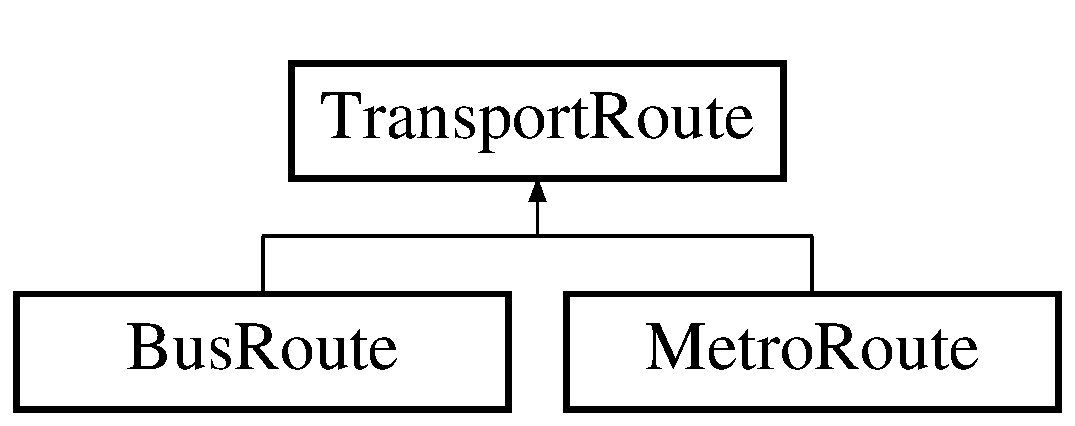
\includegraphics[height=2.000000cm]{class_transport_route}
\end{center}
\end{figure}
\subsection*{Public Member Functions}
\begin{DoxyCompactItemize}
\item 
\hyperlink{class_transport_route_a5eaa150e32517b46d0b642bdfdf28647}{Transport\+Route} (const std\+::string code, bool direction)
\begin{DoxyCompactList}\small\item\em class constructor \end{DoxyCompactList}\item 
\hypertarget{class_transport_route_a7b33d609c63e776244eca94632371a9f}{}const std\+::string \& \hyperlink{class_transport_route_a7b33d609c63e776244eca94632371a9f}{get\+Code} () const \label{class_transport_route_a7b33d609c63e776244eca94632371a9f}

\begin{DoxyCompactList}\small\item\em returns the route\textquotesingle{}s code \end{DoxyCompactList}\item 
virtual void \hyperlink{class_transport_route_a79f31c2682d702c1c0a44baed7dbf520}{add\+Stop} (\hyperlink{class_transport_stop}{Transport\+Stop} $\ast$transport\+Stop)
\begin{DoxyCompactList}\small\item\em adds a stop to the route \end{DoxyCompactList}\item 
void \hyperlink{class_transport_route_a3a358665ed7bf5d69d7135f4032c5da0}{set\+Stops} (std\+::vector$<$ \hyperlink{class_transport_stop}{Transport\+Stop} $\ast$ $>$ stops)
\begin{DoxyCompactList}\small\item\em sets the route\textquotesingle{}s stops to a given vector \end{DoxyCompactList}\item 
const std\+::vector$<$ \hyperlink{class_transport_stop}{Transport\+Stop} $\ast$ $>$ \& \hyperlink{class_transport_route_ada9ff1cd5c1a2c9ae57f6371a18f864f}{get\+Stops} () const 
\begin{DoxyCompactList}\small\item\em gets the set of stops of the route \end{DoxyCompactList}\item 
\hypertarget{class_transport_route_a76a8834e9595e973f61f3376ff3d9d34}{}virtual double \hyperlink{class_transport_route_a76a8834e9595e973f61f3376ff3d9d34}{get\+Speed} () const =0\label{class_transport_route_a76a8834e9595e973f61f3376ff3d9d34}

\begin{DoxyCompactList}\small\item\em returns the speed of the route\textquotesingle{}s transport \end{DoxyCompactList}\item 
\hypertarget{class_transport_route_a824d48902634ab05f08c348583584466}{}virtual \hyperlink{class_transport_route_a824d48902634ab05f08c348583584466}{$\sim$\+Transport\+Route} ()\label{class_transport_route_a824d48902634ab05f08c348583584466}

\begin{DoxyCompactList}\small\item\em class destructor \end{DoxyCompactList}\end{DoxyCompactItemize}
\subsection*{Protected Attributes}
\begin{DoxyCompactItemize}
\item 
\hypertarget{class_transport_route_a6184b1d4457a4a986619b9ab0c720461}{}std\+::string {\bfseries code}\label{class_transport_route_a6184b1d4457a4a986619b9ab0c720461}

\item 
\hypertarget{class_transport_route_a3b429737a6897a21ef4ef328e9a517db}{}bool {\bfseries direction}\label{class_transport_route_a3b429737a6897a21ef4ef328e9a517db}

\item 
\hypertarget{class_transport_route_a6d5816ad9c6821cd5bea3a5cf8ca7cd6}{}std\+::vector$<$ \hyperlink{class_transport_stop}{Transport\+Stop} $\ast$ $>$ {\bfseries transport\+Stops}\label{class_transport_route_a6d5816ad9c6821cd5bea3a5cf8ca7cd6}

\end{DoxyCompactItemize}


\subsection{Detailed Description}
represents a route, i.\+e., the set of stops that a \char`\"{}line\char`\"{} is made of 

\subsection{Constructor \& Destructor Documentation}
\hypertarget{class_transport_route_a5eaa150e32517b46d0b642bdfdf28647}{}\index{Transport\+Route@{Transport\+Route}!Transport\+Route@{Transport\+Route}}
\index{Transport\+Route@{Transport\+Route}!Transport\+Route@{Transport\+Route}}
\subsubsection[{Transport\+Route}]{\setlength{\rightskip}{0pt plus 5cm}Transport\+Route\+::\+Transport\+Route (
\begin{DoxyParamCaption}
\item[{const std\+::string}]{code, }
\item[{bool}]{direction}
\end{DoxyParamCaption}
)\hspace{0.3cm}{\ttfamily [inline]}}\label{class_transport_route_a5eaa150e32517b46d0b642bdfdf28647}


class constructor 


\begin{DoxyParams}{Parameters}
{\em code} & Codename for the route (e.\+x. 603) \\
\hline
{\em direction} & each value represents a direction, each being the reverse of the other \\
\hline
\end{DoxyParams}


\subsection{Member Function Documentation}
\hypertarget{class_transport_route_a79f31c2682d702c1c0a44baed7dbf520}{}\index{Transport\+Route@{Transport\+Route}!add\+Stop@{add\+Stop}}
\index{add\+Stop@{add\+Stop}!Transport\+Route@{Transport\+Route}}
\subsubsection[{add\+Stop}]{\setlength{\rightskip}{0pt plus 5cm}void Transport\+Route\+::add\+Stop (
\begin{DoxyParamCaption}
\item[{{\bf Transport\+Stop} $\ast$}]{transport\+Stop}
\end{DoxyParamCaption}
)\hspace{0.3cm}{\ttfamily [virtual]}}\label{class_transport_route_a79f31c2682d702c1c0a44baed7dbf520}


adds a stop to the route 


\begin{DoxyParams}{Parameters}
{\em transport\+Stop} & Stop to be added \\
\hline
\end{DoxyParams}
\hypertarget{class_transport_route_ada9ff1cd5c1a2c9ae57f6371a18f864f}{}\index{Transport\+Route@{Transport\+Route}!get\+Stops@{get\+Stops}}
\index{get\+Stops@{get\+Stops}!Transport\+Route@{Transport\+Route}}
\subsubsection[{get\+Stops}]{\setlength{\rightskip}{0pt plus 5cm}const vector$<$ {\bf Transport\+Stop} $\ast$ $>$ \& Transport\+Route\+::get\+Stops (
\begin{DoxyParamCaption}
{}
\end{DoxyParamCaption}
) const}\label{class_transport_route_ada9ff1cd5c1a2c9ae57f6371a18f864f}


gets the set of stops of the route 

\begin{DoxyReturn}{Returns}
vector of stops 
\end{DoxyReturn}
\hypertarget{class_transport_route_a3a358665ed7bf5d69d7135f4032c5da0}{}\index{Transport\+Route@{Transport\+Route}!set\+Stops@{set\+Stops}}
\index{set\+Stops@{set\+Stops}!Transport\+Route@{Transport\+Route}}
\subsubsection[{set\+Stops}]{\setlength{\rightskip}{0pt plus 5cm}void Transport\+Route\+::set\+Stops (
\begin{DoxyParamCaption}
\item[{std\+::vector$<$ {\bf Transport\+Stop} $\ast$ $>$}]{stops}
\end{DoxyParamCaption}
)}\label{class_transport_route_a3a358665ed7bf5d69d7135f4032c5da0}


sets the route\textquotesingle{}s stops to a given vector 


\begin{DoxyParams}{Parameters}
{\em stops} & vector with the new set of stops \\
\hline
\end{DoxyParams}


The documentation for this class was generated from the following files\+:\begin{DoxyCompactItemize}
\item 
C\+:/\+Users/\+André/\+Desktop/test/transport/Transport\+Route.\+h\item 
C\+:/\+Users/\+André/\+Desktop/test/transport/Transport\+Route.\+cpp\end{DoxyCompactItemize}

\hypertarget{class_transport_speeds}{}\section{Transport\+Speeds Class Reference}
\label{class_transport_speeds}\index{Transport\+Speeds@{Transport\+Speeds}}


generic inteface to preserve the speeds of the different means of transport  




{\ttfamily \#include $<$Transport\+Speeds.\+h$>$}

\subsection*{Static Public Member Functions}
\begin{DoxyCompactItemize}
\item 
\hypertarget{class_transport_speeds_adca751db60110762034338c76008801b}{}static double \hyperlink{class_transport_speeds_adca751db60110762034338c76008801b}{get\+Bus\+Speed} ()\label{class_transport_speeds_adca751db60110762034338c76008801b}

\begin{DoxyCompactList}\small\item\em Returns the estimated bus speed. \end{DoxyCompactList}\item 
\hypertarget{class_transport_speeds_a2d1b4983bdd67d6282a0439eaef4f5f6}{}static double \hyperlink{class_transport_speeds_a2d1b4983bdd67d6282a0439eaef4f5f6}{get\+Metro\+Speed} ()\label{class_transport_speeds_a2d1b4983bdd67d6282a0439eaef4f5f6}

\begin{DoxyCompactList}\small\item\em Returns the estimated metro speed. \end{DoxyCompactList}\item 
\hypertarget{class_transport_speeds_ae79691cf1d4716bbf301ebab34c2063a}{}static double \hyperlink{class_transport_speeds_ae79691cf1d4716bbf301ebab34c2063a}{get\+Walking\+Speed} ()\label{class_transport_speeds_ae79691cf1d4716bbf301ebab34c2063a}

\begin{DoxyCompactList}\small\item\em Returns the estimated walking speed. \end{DoxyCompactList}\item 
\hypertarget{class_transport_speeds_a799464f9b86baf4d742aceefd14bf0fb}{}static double \hyperlink{class_transport_speeds_a799464f9b86baf4d742aceefd14bf0fb}{get\+Max\+Speed} ()\label{class_transport_speeds_a799464f9b86baf4d742aceefd14bf0fb}

\begin{DoxyCompactList}\small\item\em Returns the maximum of the transport\textquotesingle{}s speed. \end{DoxyCompactList}\end{DoxyCompactItemize}


\subsection{Detailed Description}
generic inteface to preserve the speeds of the different means of transport 

The documentation for this class was generated from the following files\+:\begin{DoxyCompactItemize}
\item 
C\+:/\+Users/\+André/\+Desktop/test/transport/Transport\+Speeds.\+h\item 
C\+:/\+Users/\+André/\+Desktop/test/transport/Transport\+Speeds.\+cpp\end{DoxyCompactItemize}

\hypertarget{class_transport_stop}{}\section{Transport\+Stop Class Reference}
\label{class_transport_stop}\index{Transport\+Stop@{Transport\+Stop}}


represents a transport stop of any type  




{\ttfamily \#include $<$Transport\+Stop.\+h$>$}

Inheritance diagram for Transport\+Stop\+:\begin{figure}[H]
\begin{center}
\leavevmode
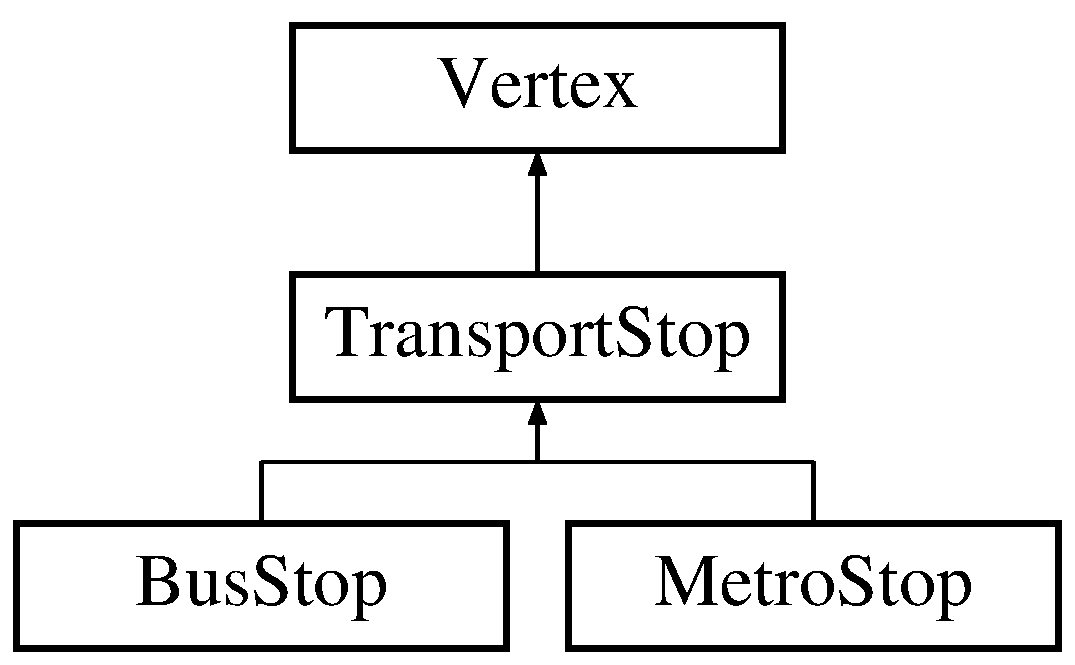
\includegraphics[height=3.000000cm]{class_transport_stop}
\end{center}
\end{figure}
\subsection*{Public Member Functions}
\begin{DoxyCompactItemize}
\item 
\hyperlink{class_transport_stop_af12f0e4489f285dc6d4ba723b8f026d1}{Transport\+Stop} (const std\+::string \&name, const \hyperlink{class_coordinates}{Coordinates} \&coords, const std\+::string \&route\+\_\+name)
\begin{DoxyCompactList}\small\item\em Default class constructor. \end{DoxyCompactList}\item 
\hypertarget{class_transport_stop_a6ff14aa5560dee86b741720a670eaf52}{}string {\bfseries get\+Route\+Name} () const \label{class_transport_stop_a6ff14aa5560dee86b741720a670eaf52}

\item 
std\+::string \hyperlink{class_transport_stop_a517602c38c031001c46bf176261fc8f3}{get\+Name} () const 
\begin{DoxyCompactList}\small\item\em Get Stop name. \end{DoxyCompactList}\item 
void \hyperlink{class_transport_stop_aaa6a1aa4b046a530ef443fcde0e04cfa}{set\+Route\+Name} (std\+::string name)
\begin{DoxyCompactList}\small\item\em set Stop name \end{DoxyCompactList}\item 
std\+::string \hyperlink{class_transport_stop_a22ed12a90c26edcc285b94bf9e345177}{get\+Route} () const 
\begin{DoxyCompactList}\small\item\em Get Stop\textquotesingle{}s route name. \end{DoxyCompactList}\item 
const \hyperlink{class_hour}{Hour} \& \hyperlink{class_transport_stop_a78b98922c8778bf781b6c194e2e6d39f}{get\+Arrival\+Time} () const 
\begin{DoxyCompactList}\small\item\em Get arrival time at stop. \end{DoxyCompactList}\item 
void \hyperlink{class_transport_stop_a5c5dabee8026a55ab610c5c57724adef}{add\+Hour} (const \hyperlink{class_hour}{Hour} \&hour)
\begin{DoxyCompactList}\small\item\em Adds an hour to the Stop. Every Stop has several \hyperlink{class_hour}{Hour}\textquotesingle{}s, representing all the moments when transports stop there. \end{DoxyCompactList}\item 
\hyperlink{class_transport_route}{Transport\+Route} $\ast$ \hyperlink{class_transport_stop_abc8403a9e107f7dcb8edc525aef7ed3c}{get\+Transport\+Route} () const 
\begin{DoxyCompactList}\small\item\em Gets the route in which the \hyperlink{class_transport_stop}{Transport\+Stop} is located. \end{DoxyCompactList}\item 
const std\+::vector$<$ \hyperlink{class_hour}{Hour} $>$ \& \hyperlink{class_transport_stop_a912501b3b2bb1a68ee443a0fb66575ad}{get\+Schedule} () const 
\begin{DoxyCompactList}\small\item\em Gets the set of times (\hyperlink{class_hour}{Hour}\textquotesingle{}s) when transports stop at this stop. \end{DoxyCompactList}\item 
void \hyperlink{class_transport_stop_a3de4faae6f399f1c7e844f3b4aeb9f56}{set\+Transport\+Route} (\hyperlink{class_transport_route}{Transport\+Route} $\ast$transport\+Route)
\begin{DoxyCompactList}\small\item\em Assign the Stop to a specific route. \end{DoxyCompactList}\item 
void \hyperlink{class_transport_stop_acf542b1d06522bd3971fc8400df331b2}{set\+Schedule} (std\+::vector$<$ \hyperlink{class_hour}{Hour} $>$ schedule)
\begin{DoxyCompactList}\small\item\em Sets the Stop\textquotesingle{}s schedule after a given one. \end{DoxyCompactList}\item 
bool \hyperlink{class_transport_stop_ade8b9ee395616a37616d05e4cb7a0421}{has\+Schedule} () const 
\begin{DoxyCompactList}\small\item\em Determines if there is any schedule assigned to the stop. \end{DoxyCompactList}\item 
virtual void \hyperlink{class_transport_stop_a862190c81155a2aca27493d268a6c1d6}{set\+Parent} (\hyperlink{class_edge}{Edge} $\ast$parent)
\begin{DoxyCompactList}\small\item\em Sets the stop\textquotesingle{}s vertex\textquotesingle{}s parent to the one specified. \end{DoxyCompactList}\item 
double \hyperlink{class_transport_stop_ac8451eda14c724048a7afcab1dfb0d3d}{calc\+Waiting\+Time} (\hyperlink{class_hour}{Hour} current\+Hour) const 
\begin{DoxyCompactList}\small\item\em Calculates the time between the arrival hour at the vertex and the next transport arriving. \end{DoxyCompactList}\item 
double \hyperlink{class_transport_stop_a2cce3ec4e28f8952981d14d5913f058e}{calculate\+H} (\hyperlink{class_vertex}{Vertex} $\ast$v)
\begin{DoxyCompactList}\small\item\em Calculates the value of the heuristic (A$\ast$ algorithm) to a certain destination vertex. \end{DoxyCompactList}\item 
virtual bool \hyperlink{class_transport_stop_a49e75a0fc1e7e2b62fe0a6894ba4e12a}{operator==} (const \hyperlink{class_transport_stop}{Transport\+Stop} \&transport\+Stop) const 
\begin{DoxyCompactList}\small\item\em Compares two \hyperlink{class_transport_stop}{Transport\+Stop}\textquotesingle{}s. \end{DoxyCompactList}\item 
\hypertarget{class_transport_stop_aa320bbb6a30f75d415cf7a37bb4ab6bd}{}virtual \hyperlink{class_transport_stop_aa320bbb6a30f75d415cf7a37bb4ab6bd}{$\sim$\+Transport\+Stop} ()\label{class_transport_stop_aa320bbb6a30f75d415cf7a37bb4ab6bd}

\begin{DoxyCompactList}\small\item\em destructor for the class \end{DoxyCompactList}\item 
void \hyperlink{class_transport_stop_aaa8fd2447f2d70ef03163e679620730a}{user\+Add\+To\+Graph} (\hyperlink{class_graph}{Graph} $\ast$g)
\begin{DoxyCompactList}\small\item\em adds the Stop\textquotesingle{}s vertex to the graph specified (used with user\textquotesingle{}s click position) \end{DoxyCompactList}\item 
void \hyperlink{class_transport_stop_a98fe1e72c2188413957cc39269a04874}{user\+Removefrom\+Graph} (\hyperlink{class_graph}{Graph} $\ast$g)
\begin{DoxyCompactList}\small\item\em removes the user added \hyperlink{class_vertex}{Vertex} from the graph \end{DoxyCompactList}\item 
virtual std\+::string \hyperlink{class_transport_stop_a245cff19d0ef473d56b93036042478ef}{get\+Name\+And\+Type} () const 
\begin{DoxyCompactList}\small\item\em returns a string with the Stop\textquotesingle{}s name and type (e.\+x. Bus\+: A\+V. D\+O\+S A\+L\+I\+A\+D\+O\+S) \end{DoxyCompactList}\item 
void \hyperlink{class_transport_stop_a55374e514b51c860efae36497636ef3d}{set\+Arrival\+Time} (\hyperlink{class_hour}{Hour} newarrival)
\begin{DoxyCompactList}\small\item\em sets the arrival time at the stop to the one specified \end{DoxyCompactList}\end{DoxyCompactItemize}
\subsection*{Protected Attributes}
\begin{DoxyCompactItemize}
\item 
\hypertarget{class_transport_stop_a1b3cfb83e138c05d6055007eb33dc7d4}{}std\+::string {\bfseries name}\label{class_transport_stop_a1b3cfb83e138c05d6055007eb33dc7d4}

\item 
\hypertarget{class_transport_stop_ab6588e60c61ec1c3e84f4d02bbd7cd5a}{}std\+::string {\bfseries route\+\_\+name}\label{class_transport_stop_ab6588e60c61ec1c3e84f4d02bbd7cd5a}

\item 
\hypertarget{class_transport_stop_ab2ed9888de5724ead0d7211d21cd8c8c}{}\hyperlink{class_transport_route}{Transport\+Route} $\ast$ {\bfseries transport\+Route}\label{class_transport_stop_ab2ed9888de5724ead0d7211d21cd8c8c}

\item 
\hypertarget{class_transport_stop_a4597a847ea2dcbfa294910658d9e1309}{}std\+::vector$<$ \hyperlink{class_hour}{Hour} $>$ {\bfseries schedule}\label{class_transport_stop_a4597a847ea2dcbfa294910658d9e1309}

\item 
\hypertarget{class_transport_stop_a38dccba7563c16328ff723468c474064}{}\hyperlink{class_hour}{Hour} {\bfseries arrival}\label{class_transport_stop_a38dccba7563c16328ff723468c474064}

\end{DoxyCompactItemize}


\subsection{Detailed Description}
represents a transport stop of any type 

\subsection{Constructor \& Destructor Documentation}
\hypertarget{class_transport_stop_af12f0e4489f285dc6d4ba723b8f026d1}{}\index{Transport\+Stop@{Transport\+Stop}!Transport\+Stop@{Transport\+Stop}}
\index{Transport\+Stop@{Transport\+Stop}!Transport\+Stop@{Transport\+Stop}}
\subsubsection[{Transport\+Stop}]{\setlength{\rightskip}{0pt plus 5cm}Transport\+Stop\+::\+Transport\+Stop (
\begin{DoxyParamCaption}
\item[{const std\+::string \&}]{name, }
\item[{const {\bf Coordinates} \&}]{coords, }
\item[{const std\+::string \&}]{route\+\_\+name}
\end{DoxyParamCaption}
)}\label{class_transport_stop_af12f0e4489f285dc6d4ba723b8f026d1}


Default class constructor. 


\begin{DoxyParams}{Parameters}
{\em name} & \hyperlink{class_transport_stop}{Transport\+Stop}\textquotesingle{}s name (e.\+x. \char`\"{}\+A\+V. D\+O\+S A\+L\+I\+A\+D\+O\+S\char`\"{}) \\
\hline
{\em coords} & \hyperlink{class_coordinates}{Coordinates} of the stop \\
\hline
{\em route\+\_\+name} & name for the Stop\textquotesingle{}s route \\
\hline
\end{DoxyParams}


\subsection{Member Function Documentation}
\hypertarget{class_transport_stop_a5c5dabee8026a55ab610c5c57724adef}{}\index{Transport\+Stop@{Transport\+Stop}!add\+Hour@{add\+Hour}}
\index{add\+Hour@{add\+Hour}!Transport\+Stop@{Transport\+Stop}}
\subsubsection[{add\+Hour}]{\setlength{\rightskip}{0pt plus 5cm}void Transport\+Stop\+::add\+Hour (
\begin{DoxyParamCaption}
\item[{const {\bf Hour} \&}]{hour}
\end{DoxyParamCaption}
)}\label{class_transport_stop_a5c5dabee8026a55ab610c5c57724adef}


Adds an hour to the Stop. Every Stop has several \hyperlink{class_hour}{Hour}\textquotesingle{}s, representing all the moments when transports stop there. 


\begin{DoxyParams}{Parameters}
{\em hour} & \hyperlink{class_hour}{Hour} to be added \\
\hline
\end{DoxyParams}
\hypertarget{class_transport_stop_a2cce3ec4e28f8952981d14d5913f058e}{}\index{Transport\+Stop@{Transport\+Stop}!calculate\+H@{calculate\+H}}
\index{calculate\+H@{calculate\+H}!Transport\+Stop@{Transport\+Stop}}
\subsubsection[{calculate\+H}]{\setlength{\rightskip}{0pt plus 5cm}double Transport\+Stop\+::calculate\+H (
\begin{DoxyParamCaption}
\item[{{\bf Vertex} $\ast$}]{v}
\end{DoxyParamCaption}
)\hspace{0.3cm}{\ttfamily [virtual]}}\label{class_transport_stop_a2cce3ec4e28f8952981d14d5913f058e}


Calculates the value of the heuristic (A$\ast$ algorithm) to a certain destination vertex. 


\begin{DoxyParams}{Parameters}
{\em v} & destination vertex \\
\hline
\end{DoxyParams}
\begin{DoxyReturn}{Returns}
value of the heuristic 
\end{DoxyReturn}


Reimplemented from \hyperlink{class_vertex_a17ef9b29d37ff0ddbc769802b2fb307e}{Vertex}.

\hypertarget{class_transport_stop_ac8451eda14c724048a7afcab1dfb0d3d}{}\index{Transport\+Stop@{Transport\+Stop}!calc\+Waiting\+Time@{calc\+Waiting\+Time}}
\index{calc\+Waiting\+Time@{calc\+Waiting\+Time}!Transport\+Stop@{Transport\+Stop}}
\subsubsection[{calc\+Waiting\+Time}]{\setlength{\rightskip}{0pt plus 5cm}double Transport\+Stop\+::calc\+Waiting\+Time (
\begin{DoxyParamCaption}
\item[{{\bf Hour}}]{current\+Hour}
\end{DoxyParamCaption}
) const}\label{class_transport_stop_ac8451eda14c724048a7afcab1dfb0d3d}


Calculates the time between the arrival hour at the vertex and the next transport arriving. 


\begin{DoxyParams}{Parameters}
{\em current\+Hour} & time of arrival at the stop \\
\hline
\end{DoxyParams}
\begin{DoxyReturn}{Returns}
ammount of seconds between the current\+Hour and the next transport 
\end{DoxyReturn}
\hypertarget{class_transport_stop_a78b98922c8778bf781b6c194e2e6d39f}{}\index{Transport\+Stop@{Transport\+Stop}!get\+Arrival\+Time@{get\+Arrival\+Time}}
\index{get\+Arrival\+Time@{get\+Arrival\+Time}!Transport\+Stop@{Transport\+Stop}}
\subsubsection[{get\+Arrival\+Time}]{\setlength{\rightskip}{0pt plus 5cm}const {\bf Hour}\& Transport\+Stop\+::get\+Arrival\+Time (
\begin{DoxyParamCaption}
{}
\end{DoxyParamCaption}
) const\hspace{0.3cm}{\ttfamily [inline]}}\label{class_transport_stop_a78b98922c8778bf781b6c194e2e6d39f}


Get arrival time at stop. 

\begin{DoxyReturn}{Returns}
The \hyperlink{class_hour}{Hour} the path arrived at the stop during path calculation. 
\end{DoxyReturn}
\hypertarget{class_transport_stop_a517602c38c031001c46bf176261fc8f3}{}\index{Transport\+Stop@{Transport\+Stop}!get\+Name@{get\+Name}}
\index{get\+Name@{get\+Name}!Transport\+Stop@{Transport\+Stop}}
\subsubsection[{get\+Name}]{\setlength{\rightskip}{0pt plus 5cm}std\+::string Transport\+Stop\+::get\+Name (
\begin{DoxyParamCaption}
{}
\end{DoxyParamCaption}
) const\hspace{0.3cm}{\ttfamily [inline]}}\label{class_transport_stop_a517602c38c031001c46bf176261fc8f3}


Get Stop name. 

\begin{DoxyReturn}{Returns}
Name of the transport stop 
\end{DoxyReturn}
\hypertarget{class_transport_stop_a245cff19d0ef473d56b93036042478ef}{}\index{Transport\+Stop@{Transport\+Stop}!get\+Name\+And\+Type@{get\+Name\+And\+Type}}
\index{get\+Name\+And\+Type@{get\+Name\+And\+Type}!Transport\+Stop@{Transport\+Stop}}
\subsubsection[{get\+Name\+And\+Type}]{\setlength{\rightskip}{0pt plus 5cm}virtual std\+::string Transport\+Stop\+::get\+Name\+And\+Type (
\begin{DoxyParamCaption}
{}
\end{DoxyParamCaption}
) const\hspace{0.3cm}{\ttfamily [inline]}, {\ttfamily [virtual]}}\label{class_transport_stop_a245cff19d0ef473d56b93036042478ef}


returns a string with the Stop\textquotesingle{}s name and type (e.\+x. Bus\+: A\+V. D\+O\+S A\+L\+I\+A\+D\+O\+S) 

\begin{DoxyReturn}{Returns}
string with the specified text 
\end{DoxyReturn}


Reimplemented in \hyperlink{class_bus_stop_a508c7cf008dcb6072ce4a5179cefd42d}{Bus\+Stop}, and \hyperlink{class_metro_stop_ab2805dfc9f452e981ca71028c64cef38}{Metro\+Stop}.

\hypertarget{class_transport_stop_a22ed12a90c26edcc285b94bf9e345177}{}\index{Transport\+Stop@{Transport\+Stop}!get\+Route@{get\+Route}}
\index{get\+Route@{get\+Route}!Transport\+Stop@{Transport\+Stop}}
\subsubsection[{get\+Route}]{\setlength{\rightskip}{0pt plus 5cm}std\+::string Transport\+Stop\+::get\+Route (
\begin{DoxyParamCaption}
{}
\end{DoxyParamCaption}
) const\hspace{0.3cm}{\ttfamily [inline]}}\label{class_transport_stop_a22ed12a90c26edcc285b94bf9e345177}


Get Stop\textquotesingle{}s route name. 

\begin{DoxyReturn}{Returns}
Name of the transport stop route 
\end{DoxyReturn}
\hypertarget{class_transport_stop_a912501b3b2bb1a68ee443a0fb66575ad}{}\index{Transport\+Stop@{Transport\+Stop}!get\+Schedule@{get\+Schedule}}
\index{get\+Schedule@{get\+Schedule}!Transport\+Stop@{Transport\+Stop}}
\subsubsection[{get\+Schedule}]{\setlength{\rightskip}{0pt plus 5cm}const vector$<$ {\bf Hour} $>$ \& Transport\+Stop\+::get\+Schedule (
\begin{DoxyParamCaption}
{}
\end{DoxyParamCaption}
) const}\label{class_transport_stop_a912501b3b2bb1a68ee443a0fb66575ad}


Gets the set of times (\hyperlink{class_hour}{Hour}\textquotesingle{}s) when transports stop at this stop. 

\begin{DoxyReturn}{Returns}
vector of \hyperlink{class_hour}{Hour} objets representing the schedule 
\end{DoxyReturn}
\hypertarget{class_transport_stop_abc8403a9e107f7dcb8edc525aef7ed3c}{}\index{Transport\+Stop@{Transport\+Stop}!get\+Transport\+Route@{get\+Transport\+Route}}
\index{get\+Transport\+Route@{get\+Transport\+Route}!Transport\+Stop@{Transport\+Stop}}
\subsubsection[{get\+Transport\+Route}]{\setlength{\rightskip}{0pt plus 5cm}{\bf Transport\+Route} $\ast$ Transport\+Stop\+::get\+Transport\+Route (
\begin{DoxyParamCaption}
{}
\end{DoxyParamCaption}
) const}\label{class_transport_stop_abc8403a9e107f7dcb8edc525aef7ed3c}


Gets the route in which the \hyperlink{class_transport_stop}{Transport\+Stop} is located. 

\begin{DoxyReturn}{Returns}
Stop\textquotesingle{}s route 
\end{DoxyReturn}
\hypertarget{class_transport_stop_ade8b9ee395616a37616d05e4cb7a0421}{}\index{Transport\+Stop@{Transport\+Stop}!has\+Schedule@{has\+Schedule}}
\index{has\+Schedule@{has\+Schedule}!Transport\+Stop@{Transport\+Stop}}
\subsubsection[{has\+Schedule}]{\setlength{\rightskip}{0pt plus 5cm}bool Transport\+Stop\+::has\+Schedule (
\begin{DoxyParamCaption}
{}
\end{DoxyParamCaption}
) const\hspace{0.3cm}{\ttfamily [inline]}}\label{class_transport_stop_ade8b9ee395616a37616d05e4cb7a0421}


Determines if there is any schedule assigned to the stop. 

\begin{DoxyReturn}{Returns}
true when the stop has a schedule, false otherwise 
\end{DoxyReturn}
\hypertarget{class_transport_stop_a49e75a0fc1e7e2b62fe0a6894ba4e12a}{}\index{Transport\+Stop@{Transport\+Stop}!operator==@{operator==}}
\index{operator==@{operator==}!Transport\+Stop@{Transport\+Stop}}
\subsubsection[{operator==}]{\setlength{\rightskip}{0pt plus 5cm}bool Transport\+Stop\+::operator== (
\begin{DoxyParamCaption}
\item[{const {\bf Transport\+Stop} \&}]{transport\+Stop}
\end{DoxyParamCaption}
) const\hspace{0.3cm}{\ttfamily [virtual]}}\label{class_transport_stop_a49e75a0fc1e7e2b62fe0a6894ba4e12a}


Compares two \hyperlink{class_transport_stop}{Transport\+Stop}\textquotesingle{}s. 


\begin{DoxyParams}{Parameters}
{\em transport\+Stop} & Stop to compare to \\
\hline
\end{DoxyParams}
\begin{DoxyReturn}{Returns}
true if both are equal, false otherwise 
\end{DoxyReturn}
\hypertarget{class_transport_stop_a55374e514b51c860efae36497636ef3d}{}\index{Transport\+Stop@{Transport\+Stop}!set\+Arrival\+Time@{set\+Arrival\+Time}}
\index{set\+Arrival\+Time@{set\+Arrival\+Time}!Transport\+Stop@{Transport\+Stop}}
\subsubsection[{set\+Arrival\+Time}]{\setlength{\rightskip}{0pt plus 5cm}void Transport\+Stop\+::set\+Arrival\+Time (
\begin{DoxyParamCaption}
\item[{{\bf Hour}}]{newarrival}
\end{DoxyParamCaption}
)\hspace{0.3cm}{\ttfamily [inline]}}\label{class_transport_stop_a55374e514b51c860efae36497636ef3d}


sets the arrival time at the stop to the one specified 


\begin{DoxyParams}{Parameters}
{\em newarrival} & \hyperlink{class_hour}{Hour} value to be set \\
\hline
\end{DoxyParams}
\hypertarget{class_transport_stop_a862190c81155a2aca27493d268a6c1d6}{}\index{Transport\+Stop@{Transport\+Stop}!set\+Parent@{set\+Parent}}
\index{set\+Parent@{set\+Parent}!Transport\+Stop@{Transport\+Stop}}
\subsubsection[{set\+Parent}]{\setlength{\rightskip}{0pt plus 5cm}void Transport\+Stop\+::set\+Parent (
\begin{DoxyParamCaption}
\item[{{\bf Edge} $\ast$}]{parent}
\end{DoxyParamCaption}
)\hspace{0.3cm}{\ttfamily [virtual]}}\label{class_transport_stop_a862190c81155a2aca27493d268a6c1d6}


Sets the stop\textquotesingle{}s vertex\textquotesingle{}s parent to the one specified. 


\begin{DoxyParams}{Parameters}
{\em parent} & \hyperlink{class_edge}{Edge} to be assigned as parent for the vertex \\
\hline
\end{DoxyParams}


Reimplemented from \hyperlink{class_vertex_a330546da58f086e183ae8ee41f5eb7fb}{Vertex}.

\hypertarget{class_transport_stop_aaa6a1aa4b046a530ef443fcde0e04cfa}{}\index{Transport\+Stop@{Transport\+Stop}!set\+Route\+Name@{set\+Route\+Name}}
\index{set\+Route\+Name@{set\+Route\+Name}!Transport\+Stop@{Transport\+Stop}}
\subsubsection[{set\+Route\+Name}]{\setlength{\rightskip}{0pt plus 5cm}void Transport\+Stop\+::set\+Route\+Name (
\begin{DoxyParamCaption}
\item[{std\+::string}]{name}
\end{DoxyParamCaption}
)\hspace{0.3cm}{\ttfamily [inline]}}\label{class_transport_stop_aaa6a1aa4b046a530ef443fcde0e04cfa}


set Stop name 

\begin{DoxyReturn}{Returns}
Name of the transport stop 
\end{DoxyReturn}
\hypertarget{class_transport_stop_acf542b1d06522bd3971fc8400df331b2}{}\index{Transport\+Stop@{Transport\+Stop}!set\+Schedule@{set\+Schedule}}
\index{set\+Schedule@{set\+Schedule}!Transport\+Stop@{Transport\+Stop}}
\subsubsection[{set\+Schedule}]{\setlength{\rightskip}{0pt plus 5cm}void Transport\+Stop\+::set\+Schedule (
\begin{DoxyParamCaption}
\item[{std\+::vector$<$ {\bf Hour} $>$}]{schedule}
\end{DoxyParamCaption}
)\hspace{0.3cm}{\ttfamily [inline]}}\label{class_transport_stop_acf542b1d06522bd3971fc8400df331b2}


Sets the Stop\textquotesingle{}s schedule after a given one. 


\begin{DoxyParams}{Parameters}
{\em schedule} & Vector of Hours to be set as the stop\textquotesingle{}s schedule \\
\hline
\end{DoxyParams}
\hypertarget{class_transport_stop_a3de4faae6f399f1c7e844f3b4aeb9f56}{}\index{Transport\+Stop@{Transport\+Stop}!set\+Transport\+Route@{set\+Transport\+Route}}
\index{set\+Transport\+Route@{set\+Transport\+Route}!Transport\+Stop@{Transport\+Stop}}
\subsubsection[{set\+Transport\+Route}]{\setlength{\rightskip}{0pt plus 5cm}void Transport\+Stop\+::set\+Transport\+Route (
\begin{DoxyParamCaption}
\item[{{\bf Transport\+Route} $\ast$}]{transport\+Route}
\end{DoxyParamCaption}
)}\label{class_transport_stop_a3de4faae6f399f1c7e844f3b4aeb9f56}


Assign the Stop to a specific route. 


\begin{DoxyParams}{Parameters}
{\em transport\+Route} & Route the stop is to be assigned to \\
\hline
\end{DoxyParams}
\hypertarget{class_transport_stop_aaa8fd2447f2d70ef03163e679620730a}{}\index{Transport\+Stop@{Transport\+Stop}!user\+Add\+To\+Graph@{user\+Add\+To\+Graph}}
\index{user\+Add\+To\+Graph@{user\+Add\+To\+Graph}!Transport\+Stop@{Transport\+Stop}}
\subsubsection[{user\+Add\+To\+Graph}]{\setlength{\rightskip}{0pt plus 5cm}void Transport\+Stop\+::user\+Add\+To\+Graph (
\begin{DoxyParamCaption}
\item[{{\bf Graph} $\ast$}]{g}
\end{DoxyParamCaption}
)}\label{class_transport_stop_aaa8fd2447f2d70ef03163e679620730a}


adds the Stop\textquotesingle{}s vertex to the graph specified (used with user\textquotesingle{}s click position) 


\begin{DoxyParams}{Parameters}
{\em g} & \hyperlink{class_graph}{Graph} to be changed \\
\hline
\end{DoxyParams}
\hypertarget{class_transport_stop_a98fe1e72c2188413957cc39269a04874}{}\index{Transport\+Stop@{Transport\+Stop}!user\+Removefrom\+Graph@{user\+Removefrom\+Graph}}
\index{user\+Removefrom\+Graph@{user\+Removefrom\+Graph}!Transport\+Stop@{Transport\+Stop}}
\subsubsection[{user\+Removefrom\+Graph}]{\setlength{\rightskip}{0pt plus 5cm}void Transport\+Stop\+::user\+Removefrom\+Graph (
\begin{DoxyParamCaption}
\item[{{\bf Graph} $\ast$}]{g}
\end{DoxyParamCaption}
)}\label{class_transport_stop_a98fe1e72c2188413957cc39269a04874}


removes the user added \hyperlink{class_vertex}{Vertex} from the graph 


\begin{DoxyParams}{Parameters}
{\em g} & \hyperlink{class_graph}{Graph} to remove vertex from \\
\hline
\end{DoxyParams}


The documentation for this class was generated from the following files\+:\begin{DoxyCompactItemize}
\item 
C\+:/\+Users/\+André/\+Desktop/test/transport/Transport\+Stop.\+h\item 
C\+:/\+Users/\+André/\+Desktop/test/transport/Transport\+Stop.\+cpp\end{DoxyCompactItemize}

\hypertarget{class_transport_stop_dist_compare}{}\section{Transport\+Stop\+Dist\+Compare Class Reference}
\label{class_transport_stop_dist_compare}\index{Transport\+Stop\+Dist\+Compare@{Transport\+Stop\+Dist\+Compare}}
\subsection*{Public Member Functions}
\begin{DoxyCompactItemize}
\item 
bool \hyperlink{class_transport_stop_dist_compare_a441844e7592efcc6be894750f9d7ff27}{operator()} (const \hyperlink{class_transport_stop}{Transport\+Stop} $\ast$ts1, const \hyperlink{class_transport_stop}{Transport\+Stop} $\ast$ts2)
\begin{DoxyCompactList}\small\item\em compares the distance between the two transport stops and the reference point \end{DoxyCompactList}\end{DoxyCompactItemize}
\subsection*{Static Public Attributes}
\begin{DoxyCompactItemize}
\item 
\hypertarget{class_transport_stop_dist_compare_aa004cc533ccecc23dd95d37d193da79d}{}static \hyperlink{class_coordinates}{Coordinates} {\bfseries reference} = \hyperlink{class_coordinates}{Coordinates}(0, 0)\label{class_transport_stop_dist_compare_aa004cc533ccecc23dd95d37d193da79d}

\end{DoxyCompactItemize}


\subsection{Member Function Documentation}
\hypertarget{class_transport_stop_dist_compare_a441844e7592efcc6be894750f9d7ff27}{}\index{Transport\+Stop\+Dist\+Compare@{Transport\+Stop\+Dist\+Compare}!operator()@{operator()}}
\index{operator()@{operator()}!Transport\+Stop\+Dist\+Compare@{Transport\+Stop\+Dist\+Compare}}
\subsubsection[{operator()}]{\setlength{\rightskip}{0pt plus 5cm}bool Transport\+Stop\+Dist\+Compare\+::operator() (
\begin{DoxyParamCaption}
\item[{const {\bf Transport\+Stop} $\ast$}]{ts1, }
\item[{const {\bf Transport\+Stop} $\ast$}]{ts2}
\end{DoxyParamCaption}
)\hspace{0.3cm}{\ttfamily [inline]}}\label{class_transport_stop_dist_compare_a441844e7592efcc6be894750f9d7ff27}


compares the distance between the two transport stops and the reference point 


\begin{DoxyParams}{Parameters}
{\em ts1} & first transportstop \\
\hline
{\em ts2} & second transportstop \\
\hline
\end{DoxyParams}
\begin{DoxyReturn}{Returns}
true if ts1 is closest to ts2 
\end{DoxyReturn}


The documentation for this class was generated from the following files\+:\begin{DoxyCompactItemize}
\item 
C\+:/\+Users/\+André/\+Desktop/test/transport/Transport\+Stop.\+h\item 
C\+:/\+Users/\+André/\+Desktop/test/transport/Transport\+Stop.\+cpp\end{DoxyCompactItemize}

\hypertarget{class_vertex}{}\section{Vertex Class Reference}
\label{class_vertex}\index{Vertex@{Vertex}}


generic inteface of a graph vertex  




{\ttfamily \#include $<$Vertex.\+h$>$}

Inheritance diagram for Vertex\+:\begin{figure}[H]
\begin{center}
\leavevmode
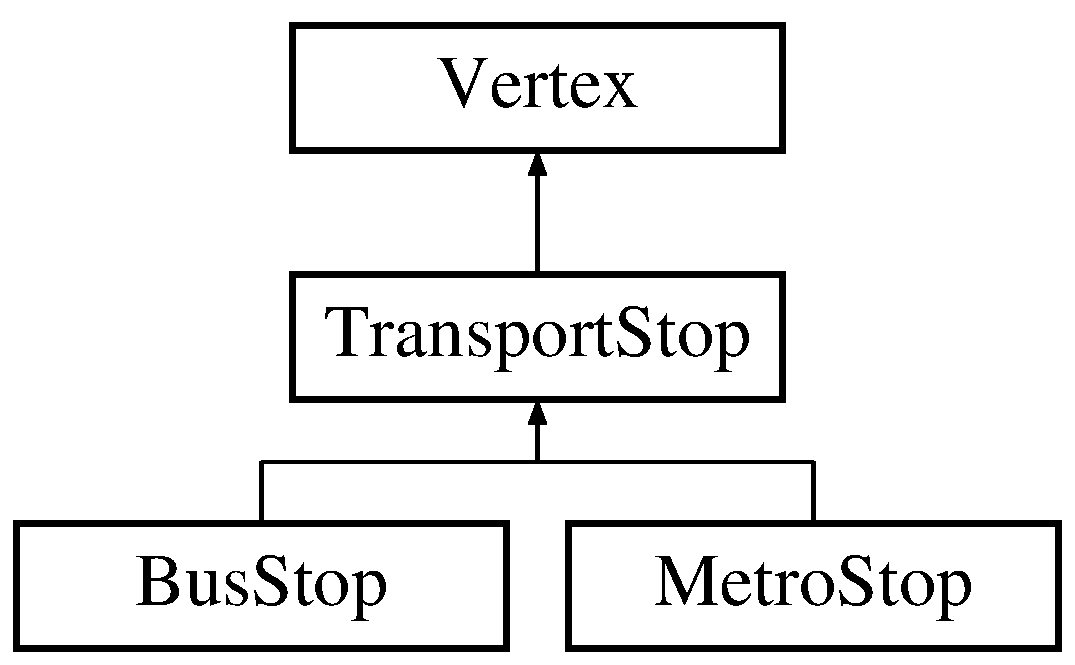
\includegraphics[height=3.000000cm]{class_vertex}
\end{center}
\end{figure}
\subsection*{Classes}
\begin{DoxyCompactItemize}
\item 
struct \hyperlink{struct_vertex_1_1_a_star_comp}{A\+Star\+Comp}
\begin{DoxyCompactList}\small\item\em comparison struct for ordering of vertex pointers for use in A$\ast$ algorithm \end{DoxyCompactList}\item 
struct \hyperlink{struct_vertex_1_1_dijs_comp}{Dijs\+Comp}
\begin{DoxyCompactList}\small\item\em comparison struct for ordering of vertex pointers for use in Dijkstra\textquotesingle{}s algorithm \end{DoxyCompactList}\end{DoxyCompactItemize}
\subsection*{Public Member Functions}
\begin{DoxyCompactItemize}
\item 
\hyperlink{class_vertex_ae86a694fcad11ed1078c3761deaa0d1f}{Vertex} (const \hyperlink{class_coordinates}{Coordinates} \&coords)
\begin{DoxyCompactList}\small\item\em vertex constructor \end{DoxyCompactList}\item 
std\+::vector$<$ \hyperlink{class_edge}{Edge} $\ast$ $>$ \hyperlink{class_vertex_abe6306ddafb1250080563fbe645e382f}{get\+Adj} () const 
\begin{DoxyCompactList}\small\item\em get the edges that exit this vertex \end{DoxyCompactList}\item 
void \hyperlink{class_vertex_a24b15df4ff9b1969ccad22db8187273a}{add\+Adj} (\hyperlink{class_vertex}{Vertex} $\ast$v, double weight=0)
\begin{DoxyCompactList}\small\item\em add vertex to list of adjacents \end{DoxyCompactList}\item 
void \hyperlink{class_vertex_a8680da16057ec72dde00eb7ebf43e4d7}{add\+Edge} (\hyperlink{class_edge}{Edge} $\ast$edge)
\begin{DoxyCompactList}\small\item\em add edge to vertex \end{DoxyCompactList}\item 
\hyperlink{class_coordinates}{Coordinates} \hyperlink{class_vertex_a383f8757d8642562efb1cd36523623fb}{get\+Coords} () const 
\begin{DoxyCompactList}\small\item\em get the coordinates of this vertex \end{DoxyCompactList}\item 
double \hyperlink{class_vertex_a5df81beb3e6f7577891665142da3a000}{get\+Render\+X} () const 
\begin{DoxyCompactList}\small\item\em get x position of vertex \end{DoxyCompactList}\item 
double \hyperlink{class_vertex_a1b50b9fe0d0581df53751c5085f4e077}{get\+Render\+Y} () const 
\begin{DoxyCompactList}\small\item\em get y position of vertex \end{DoxyCompactList}\item 
unsigned int \hyperlink{class_vertex_ab265879de21dc8c08ece53523ceab31f}{get\+Index} () const 
\begin{DoxyCompactList}\small\item\em get index of vertex, its position in vertex\+Set of its containing graph \end{DoxyCompactList}\item 
virtual unsigned int \hyperlink{class_vertex_a4f6652186dc60a82b78a631cf0fcbed7}{get\+Render\+X} ()
\begin{DoxyCompactList}\small\item\em get x position of vertex \end{DoxyCompactList}\item 
virtual unsigned int \hyperlink{class_vertex_a7daa9b7383e6514bdf3dcfa9d755cd64}{get\+Render\+Y} ()
\begin{DoxyCompactList}\small\item\em get x position of vertex \end{DoxyCompactList}\item 
\hypertarget{class_vertex_ad7a0ce588b7f688dc4488a0f567d9155}{}virtual \hyperlink{class_vertex_ad7a0ce588b7f688dc4488a0f567d9155}{$\sim$\+Vertex} ()\label{class_vertex_ad7a0ce588b7f688dc4488a0f567d9155}

\begin{DoxyCompactList}\small\item\em destructor for class \end{DoxyCompactList}\item 
void \hyperlink{class_vertex_a587727c9d4e4cb9bbd7d9cda6ad2bc50}{set\+Index} (unsigned int index)
\begin{DoxyCompactList}\small\item\em set index of vertex, its position in vertex\+Set of its containing graph \end{DoxyCompactList}\item 
double \hyperlink{class_vertex_ab014e707dfcbee8a7a0e6a4251600dce}{get\+Best\+Weight} () const 
\begin{DoxyCompactList}\small\item\em get the best value for edge weight obtained during the course of an algorithm \end{DoxyCompactList}\item 
void \hyperlink{class_vertex_a72550c460ff084a7d167688bd9b3d7c2}{set\+Best\+Weight} (double best\+Weight)
\begin{DoxyCompactList}\small\item\em set the best value for edge weight obtained during the course of an algorithm \end{DoxyCompactList}\item 
\hypertarget{class_vertex_ab9e1ca696e9322fd8d32316ef752eee4}{}void \hyperlink{class_vertex_ab9e1ca696e9322fd8d32316ef752eee4}{reset\+Best\+Weight} ()\label{class_vertex_ab9e1ca696e9322fd8d32316ef752eee4}

\begin{DoxyCompactList}\small\item\em reset the best value for edge weight obtained during the course of an algorithm, positive infinity, vertex unreached \end{DoxyCompactList}\item 
\hyperlink{class_edge}{Edge} $\ast$ \hyperlink{class_vertex_afa6a4c6fa429a1b1f4d707a226e0fc9a}{get\+Parent} () const 
\begin{DoxyCompactList}\small\item\em get the last edge of the path that produced the lowest weight so far \end{DoxyCompactList}\item 
virtual void \hyperlink{class_vertex_a330546da58f086e183ae8ee41f5eb7fb}{set\+Parent} (\hyperlink{class_edge}{Edge} $\ast$parent)
\begin{DoxyCompactList}\small\item\em set the last edge of the path that produced the lowest weight so far \end{DoxyCompactList}\item 
\hypertarget{class_vertex_a42a3c40617d40971eb5745738166b3a8}{}void \hyperlink{class_vertex_a42a3c40617d40971eb5745738166b3a8}{reset\+Processed} ()\label{class_vertex_a42a3c40617d40971eb5745738166b3a8}

\begin{DoxyCompactList}\small\item\em set the number of times the vertex has been processed to 0 \end{DoxyCompactList}\item 
\hypertarget{class_vertex_ae43f5e09052c8ae57f98f00d60d6c053}{}int \hyperlink{class_vertex_ae43f5e09052c8ae57f98f00d60d6c053}{get\+Processed} () const \label{class_vertex_ae43f5e09052c8ae57f98f00d60d6c053}

\begin{DoxyCompactList}\small\item\em get the number of times the vertex has been processed since the counter was reset \end{DoxyCompactList}\item 
\hypertarget{class_vertex_adf49c348f0412081ce1a479724797894}{}void \hyperlink{class_vertex_adf49c348f0412081ce1a479724797894}{inc\+Processed} ()\label{class_vertex_adf49c348f0412081ce1a479724797894}

\begin{DoxyCompactList}\small\item\em increment the number of times the vertex has been processed since the counter was reset \end{DoxyCompactList}\item 
\hypertarget{class_vertex_a625f7958571b972389493203547c5b42}{}int \hyperlink{class_vertex_a625f7958571b972389493203547c5b42}{get\+Visits} () const \label{class_vertex_a625f7958571b972389493203547c5b42}

\begin{DoxyCompactList}\small\item\em get the number of times the vertex has been visited since the counter was reset \end{DoxyCompactList}\item 
\hypertarget{class_vertex_a422fe102e53b0f35653fd22f250be8cf}{}void \hyperlink{class_vertex_a422fe102e53b0f35653fd22f250be8cf}{reset\+Visits} ()\label{class_vertex_a422fe102e53b0f35653fd22f250be8cf}

\begin{DoxyCompactList}\small\item\em reset the number of times the vertex has been visited \end{DoxyCompactList}\item 
\hypertarget{class_vertex_a6367bff88517bb53500eb1648c18b82e}{}void \hyperlink{class_vertex_a6367bff88517bb53500eb1648c18b82e}{inc\+Visits} ()\label{class_vertex_a6367bff88517bb53500eb1648c18b82e}

\begin{DoxyCompactList}\small\item\em increment the number of times the vertex has been visited \end{DoxyCompactList}\item 
virtual double \hyperlink{class_vertex_a17ef9b29d37ff0ddbc769802b2fb307e}{calculate\+H} (\hyperlink{class_vertex}{Vertex} $\ast$v)
\begin{DoxyCompactList}\small\item\em calculate and store heuristic value from this vertex to a destination vertex \end{DoxyCompactList}\item 
double \hyperlink{class_vertex_aaa2fa5fe6903406f9bef70617fb3a16e}{get\+Stored\+H} () const 
\begin{DoxyCompactList}\small\item\em retrive stored heuristic value \end{DoxyCompactList}\item 
\hypertarget{class_vertex_ab46427731c017d3cb63bdb9cf951bd71}{}void \hyperlink{class_vertex_ab46427731c017d3cb63bdb9cf951bd71}{reset\+Stored\+H} ()\label{class_vertex_ab46427731c017d3cb63bdb9cf951bd71}

\begin{DoxyCompactList}\small\item\em retrive stored heuristic value \end{DoxyCompactList}\item 
\hypertarget{class_vertex_a6c6def262e5b1950fc71bafe1d529899}{}void {\bfseries remove\+Edge} (int i)\label{class_vertex_a6c6def262e5b1950fc71bafe1d529899}

\end{DoxyCompactItemize}
\subsection*{Protected Attributes}
\begin{DoxyCompactItemize}
\item 
\hypertarget{class_vertex_a51e8014823c3d58071383d89bc3340a4}{}\hyperlink{class_coordinates}{Coordinates} {\bfseries coords}\label{class_vertex_a51e8014823c3d58071383d89bc3340a4}

\item 
\hypertarget{class_vertex_ab8a4928af1bf9d4039a55a9c938e20db}{}double {\bfseries stored\+H}\label{class_vertex_ab8a4928af1bf9d4039a55a9c938e20db}

\end{DoxyCompactItemize}


\subsection{Detailed Description}
generic inteface of a graph vertex 

\subsection{Constructor \& Destructor Documentation}
\hypertarget{class_vertex_ae86a694fcad11ed1078c3761deaa0d1f}{}\index{Vertex@{Vertex}!Vertex@{Vertex}}
\index{Vertex@{Vertex}!Vertex@{Vertex}}
\subsubsection[{Vertex}]{\setlength{\rightskip}{0pt plus 5cm}Vertex\+::\+Vertex (
\begin{DoxyParamCaption}
\item[{const {\bf Coordinates} \&}]{coords}
\end{DoxyParamCaption}
)}\label{class_vertex_ae86a694fcad11ed1078c3761deaa0d1f}


vertex constructor 


\begin{DoxyParams}{Parameters}
{\em coords} & coordinates of vertex \\
\hline
\end{DoxyParams}


\subsection{Member Function Documentation}
\hypertarget{class_vertex_a24b15df4ff9b1969ccad22db8187273a}{}\index{Vertex@{Vertex}!add\+Adj@{add\+Adj}}
\index{add\+Adj@{add\+Adj}!Vertex@{Vertex}}
\subsubsection[{add\+Adj}]{\setlength{\rightskip}{0pt plus 5cm}void Vertex\+::add\+Adj (
\begin{DoxyParamCaption}
\item[{{\bf Vertex} $\ast$}]{v, }
\item[{double}]{weight = {\ttfamily 0}}
\end{DoxyParamCaption}
)}\label{class_vertex_a24b15df4ff9b1969ccad22db8187273a}


add vertex to list of adjacents 


\begin{DoxyParams}{Parameters}
{\em v} & vertex to add \\
\hline
{\em weight} & weight of edge to create \\
\hline
\end{DoxyParams}
\hypertarget{class_vertex_a8680da16057ec72dde00eb7ebf43e4d7}{}\index{Vertex@{Vertex}!add\+Edge@{add\+Edge}}
\index{add\+Edge@{add\+Edge}!Vertex@{Vertex}}
\subsubsection[{add\+Edge}]{\setlength{\rightskip}{0pt plus 5cm}void Vertex\+::add\+Edge (
\begin{DoxyParamCaption}
\item[{{\bf Edge} $\ast$}]{edge}
\end{DoxyParamCaption}
)}\label{class_vertex_a8680da16057ec72dde00eb7ebf43e4d7}


add edge to vertex 


\begin{DoxyParams}{Parameters}
{\em edge} & edge to add \\
\hline
\end{DoxyParams}
\hypertarget{class_vertex_a17ef9b29d37ff0ddbc769802b2fb307e}{}\index{Vertex@{Vertex}!calculate\+H@{calculate\+H}}
\index{calculate\+H@{calculate\+H}!Vertex@{Vertex}}
\subsubsection[{calculate\+H}]{\setlength{\rightskip}{0pt plus 5cm}double Vertex\+::calculate\+H (
\begin{DoxyParamCaption}
\item[{{\bf Vertex} $\ast$}]{v}
\end{DoxyParamCaption}
)\hspace{0.3cm}{\ttfamily [virtual]}}\label{class_vertex_a17ef9b29d37ff0ddbc769802b2fb307e}


calculate and store heuristic value from this vertex to a destination vertex 


\begin{DoxyParams}{Parameters}
{\em v} & goal vertex \\
\hline
\end{DoxyParams}
\begin{DoxyReturn}{Returns}
heuristic value 
\end{DoxyReturn}


Reimplemented in \hyperlink{class_transport_stop_a2cce3ec4e28f8952981d14d5913f058e}{Transport\+Stop}.

\hypertarget{class_vertex_abe6306ddafb1250080563fbe645e382f}{}\index{Vertex@{Vertex}!get\+Adj@{get\+Adj}}
\index{get\+Adj@{get\+Adj}!Vertex@{Vertex}}
\subsubsection[{get\+Adj}]{\setlength{\rightskip}{0pt plus 5cm}std\+::vector$<$ {\bf Edge} $\ast$ $>$ Vertex\+::get\+Adj (
\begin{DoxyParamCaption}
{}
\end{DoxyParamCaption}
) const}\label{class_vertex_abe6306ddafb1250080563fbe645e382f}


get the edges that exit this vertex 

\begin{DoxyReturn}{Returns}
adjacent vertices 
\end{DoxyReturn}
\hypertarget{class_vertex_ab014e707dfcbee8a7a0e6a4251600dce}{}\index{Vertex@{Vertex}!get\+Best\+Weight@{get\+Best\+Weight}}
\index{get\+Best\+Weight@{get\+Best\+Weight}!Vertex@{Vertex}}
\subsubsection[{get\+Best\+Weight}]{\setlength{\rightskip}{0pt plus 5cm}double Vertex\+::get\+Best\+Weight (
\begin{DoxyParamCaption}
{}
\end{DoxyParamCaption}
) const}\label{class_vertex_ab014e707dfcbee8a7a0e6a4251600dce}


get the best value for edge weight obtained during the course of an algorithm 

\begin{DoxyReturn}{Returns}
best value for weight so far 
\end{DoxyReturn}
\hypertarget{class_vertex_a383f8757d8642562efb1cd36523623fb}{}\index{Vertex@{Vertex}!get\+Coords@{get\+Coords}}
\index{get\+Coords@{get\+Coords}!Vertex@{Vertex}}
\subsubsection[{get\+Coords}]{\setlength{\rightskip}{0pt plus 5cm}{\bf Coordinates} Vertex\+::get\+Coords (
\begin{DoxyParamCaption}
{}
\end{DoxyParamCaption}
) const}\label{class_vertex_a383f8757d8642562efb1cd36523623fb}


get the coordinates of this vertex 

\begin{DoxyReturn}{Returns}
coordinate of vertex 
\end{DoxyReturn}
\hypertarget{class_vertex_ab265879de21dc8c08ece53523ceab31f}{}\index{Vertex@{Vertex}!get\+Index@{get\+Index}}
\index{get\+Index@{get\+Index}!Vertex@{Vertex}}
\subsubsection[{get\+Index}]{\setlength{\rightskip}{0pt plus 5cm}unsigned int Vertex\+::get\+Index (
\begin{DoxyParamCaption}
{}
\end{DoxyParamCaption}
) const}\label{class_vertex_ab265879de21dc8c08ece53523ceab31f}


get index of vertex, its position in vertex\+Set of its containing graph 

\begin{DoxyReturn}{Returns}
index of vertex 
\end{DoxyReturn}
\hypertarget{class_vertex_afa6a4c6fa429a1b1f4d707a226e0fc9a}{}\index{Vertex@{Vertex}!get\+Parent@{get\+Parent}}
\index{get\+Parent@{get\+Parent}!Vertex@{Vertex}}
\subsubsection[{get\+Parent}]{\setlength{\rightskip}{0pt plus 5cm}{\bf Edge} $\ast$ Vertex\+::get\+Parent (
\begin{DoxyParamCaption}
{}
\end{DoxyParamCaption}
) const}\label{class_vertex_afa6a4c6fa429a1b1f4d707a226e0fc9a}


get the last edge of the path that produced the lowest weight so far 

\begin{DoxyReturn}{Returns}
edge with this vertex as dst 
\end{DoxyReturn}
\hypertarget{class_vertex_a5df81beb3e6f7577891665142da3a000}{}\index{Vertex@{Vertex}!get\+Render\+X@{get\+Render\+X}}
\index{get\+Render\+X@{get\+Render\+X}!Vertex@{Vertex}}
\subsubsection[{get\+Render\+X}]{\setlength{\rightskip}{0pt plus 5cm}double Vertex\+::get\+Render\+X (
\begin{DoxyParamCaption}
{}
\end{DoxyParamCaption}
) const}\label{class_vertex_a5df81beb3e6f7577891665142da3a000}


get x position of vertex 

\begin{DoxyReturn}{Returns}
x postiton of vertex 
\end{DoxyReturn}
\hypertarget{class_vertex_a4f6652186dc60a82b78a631cf0fcbed7}{}\index{Vertex@{Vertex}!get\+Render\+X@{get\+Render\+X}}
\index{get\+Render\+X@{get\+Render\+X}!Vertex@{Vertex}}
\subsubsection[{get\+Render\+X}]{\setlength{\rightskip}{0pt plus 5cm}unsigned int Vertex\+::get\+Render\+X (
\begin{DoxyParamCaption}
{}
\end{DoxyParamCaption}
)\hspace{0.3cm}{\ttfamily [virtual]}}\label{class_vertex_a4f6652186dc60a82b78a631cf0fcbed7}


get x position of vertex 

\begin{DoxyReturn}{Returns}
x postiton of vertex 
\end{DoxyReturn}
\hypertarget{class_vertex_a1b50b9fe0d0581df53751c5085f4e077}{}\index{Vertex@{Vertex}!get\+Render\+Y@{get\+Render\+Y}}
\index{get\+Render\+Y@{get\+Render\+Y}!Vertex@{Vertex}}
\subsubsection[{get\+Render\+Y}]{\setlength{\rightskip}{0pt plus 5cm}double Vertex\+::get\+Render\+Y (
\begin{DoxyParamCaption}
{}
\end{DoxyParamCaption}
) const}\label{class_vertex_a1b50b9fe0d0581df53751c5085f4e077}


get y position of vertex 

\begin{DoxyReturn}{Returns}
y postiton of vertex 
\end{DoxyReturn}
\hypertarget{class_vertex_a7daa9b7383e6514bdf3dcfa9d755cd64}{}\index{Vertex@{Vertex}!get\+Render\+Y@{get\+Render\+Y}}
\index{get\+Render\+Y@{get\+Render\+Y}!Vertex@{Vertex}}
\subsubsection[{get\+Render\+Y}]{\setlength{\rightskip}{0pt plus 5cm}unsigned int Vertex\+::get\+Render\+Y (
\begin{DoxyParamCaption}
{}
\end{DoxyParamCaption}
)\hspace{0.3cm}{\ttfamily [virtual]}}\label{class_vertex_a7daa9b7383e6514bdf3dcfa9d755cd64}


get x position of vertex 

\begin{DoxyReturn}{Returns}
x postiton of vertex 
\end{DoxyReturn}
\hypertarget{class_vertex_aaa2fa5fe6903406f9bef70617fb3a16e}{}\index{Vertex@{Vertex}!get\+Stored\+H@{get\+Stored\+H}}
\index{get\+Stored\+H@{get\+Stored\+H}!Vertex@{Vertex}}
\subsubsection[{get\+Stored\+H}]{\setlength{\rightskip}{0pt plus 5cm}double Vertex\+::get\+Stored\+H (
\begin{DoxyParamCaption}
{}
\end{DoxyParamCaption}
) const}\label{class_vertex_aaa2fa5fe6903406f9bef70617fb3a16e}


retrive stored heuristic value 

\begin{DoxyReturn}{Returns}
stored heuristic value 
\end{DoxyReturn}
\hypertarget{class_vertex_a72550c460ff084a7d167688bd9b3d7c2}{}\index{Vertex@{Vertex}!set\+Best\+Weight@{set\+Best\+Weight}}
\index{set\+Best\+Weight@{set\+Best\+Weight}!Vertex@{Vertex}}
\subsubsection[{set\+Best\+Weight}]{\setlength{\rightskip}{0pt plus 5cm}void Vertex\+::set\+Best\+Weight (
\begin{DoxyParamCaption}
\item[{double}]{best\+Weight}
\end{DoxyParamCaption}
)}\label{class_vertex_a72550c460ff084a7d167688bd9b3d7c2}


set the best value for edge weight obtained during the course of an algorithm 


\begin{DoxyParams}{Parameters}
{\em best\+Weight} & best value for weight so far \\
\hline
\end{DoxyParams}
\hypertarget{class_vertex_a587727c9d4e4cb9bbd7d9cda6ad2bc50}{}\index{Vertex@{Vertex}!set\+Index@{set\+Index}}
\index{set\+Index@{set\+Index}!Vertex@{Vertex}}
\subsubsection[{set\+Index}]{\setlength{\rightskip}{0pt plus 5cm}void Vertex\+::set\+Index (
\begin{DoxyParamCaption}
\item[{unsigned int}]{index}
\end{DoxyParamCaption}
)}\label{class_vertex_a587727c9d4e4cb9bbd7d9cda6ad2bc50}


set index of vertex, its position in vertex\+Set of its containing graph 


\begin{DoxyParams}{Parameters}
{\em new} & index in graph \\
\hline
\end{DoxyParams}
\hypertarget{class_vertex_a330546da58f086e183ae8ee41f5eb7fb}{}\index{Vertex@{Vertex}!set\+Parent@{set\+Parent}}
\index{set\+Parent@{set\+Parent}!Vertex@{Vertex}}
\subsubsection[{set\+Parent}]{\setlength{\rightskip}{0pt plus 5cm}void Vertex\+::set\+Parent (
\begin{DoxyParamCaption}
\item[{{\bf Edge} $\ast$}]{parent}
\end{DoxyParamCaption}
)\hspace{0.3cm}{\ttfamily [virtual]}}\label{class_vertex_a330546da58f086e183ae8ee41f5eb7fb}


set the last edge of the path that produced the lowest weight so far 

\begin{DoxyReturn}{Returns}
edge with this vertex as dst, to set as parent 
\end{DoxyReturn}


Reimplemented in \hyperlink{class_transport_stop_a862190c81155a2aca27493d268a6c1d6}{Transport\+Stop}.



The documentation for this class was generated from the following files\+:\begin{DoxyCompactItemize}
\item 
C\+:/\+Users/\+André/\+Desktop/test/graph/Vertex.\+h\item 
C\+:/\+Users/\+André/\+Desktop/test/graph/Vertex.\+cpp\end{DoxyCompactItemize}

\hypertarget{class_weight_info}{}\section{Weight\+Info Class Reference}
\label{class_weight_info}\index{Weight\+Info@{Weight\+Info}}


interface to save the user preferences about relative weights and also the different weights of an edge  




{\ttfamily \#include $<$Weight\+Info.\+h$>$}

\subsection*{Public Member Functions}
\begin{DoxyCompactItemize}
\item 
\hypertarget{class_weight_info_a926aa00bc0d9e6cc9007c9ec06bc9b73}{}\hyperlink{class_weight_info_a926aa00bc0d9e6cc9007c9ec06bc9b73}{Weight\+Info} ()\label{class_weight_info_a926aa00bc0d9e6cc9007c9ec06bc9b73}

\begin{DoxyCompactList}\small\item\em constructor \end{DoxyCompactList}\item 
double \hyperlink{class_weight_info_a71c15e39640780d0c7a6188bc9c5b1f7}{get\+Weight} () const 
\begin{DoxyCompactList}\small\item\em get the weight value \end{DoxyCompactList}\item 
double \hyperlink{class_weight_info_a95cd81eace69fa37d8200cbf503ecbbc}{get\+Cost} () const 
\begin{DoxyCompactList}\small\item\em get the monetary cost \end{DoxyCompactList}\item 
void \hyperlink{class_weight_info_abe97f95f7e4fbfda379879e56ba67b82}{set\+Cost} (double cost)
\begin{DoxyCompactList}\small\item\em set the monetary cost \end{DoxyCompactList}\item 
double \hyperlink{class_weight_info_a2939a18c59d106925c3ff1559eaae292}{get\+Distance} () const 
\begin{DoxyCompactList}\small\item\em get the distance \end{DoxyCompactList}\item 
void \hyperlink{class_weight_info_aeecd1a648ca9ca739a9009c2eff63fbb}{set\+Distance} (double distance)
\begin{DoxyCompactList}\small\item\em set the distance \end{DoxyCompactList}\item 
double \hyperlink{class_weight_info_a82dba83714cd8449f08ee632e73dd52c}{get\+Switchs} () const 
\begin{DoxyCompactList}\small\item\em get the number of switchs made \end{DoxyCompactList}\item 
void \hyperlink{class_weight_info_a2434a03bba38b88078d27c4de0a4964e}{set\+Switchs} (double switchs)
\begin{DoxyCompactList}\small\item\em set the number of switchs made \end{DoxyCompactList}\item 
double \hyperlink{class_weight_info_a97e79f7bf650ad7756d4e3257baa11da}{get\+Time} () const 
\begin{DoxyCompactList}\small\item\em get the amount of time \end{DoxyCompactList}\item 
void \hyperlink{class_weight_info_ac38800f9060360b80ee0d7547b228b60}{set\+Time} (double time)
\begin{DoxyCompactList}\small\item\em set the amount of time \end{DoxyCompactList}\item 
\hyperlink{class_weight_info}{Weight\+Info} \hyperlink{class_weight_info_a70f3f16d32900beda84d378e911de764}{operator+} (const \hyperlink{class_weight_info}{Weight\+Info} \&w) const 
\begin{DoxyCompactList}\small\item\em add two Weight\+Infos by adding their components \end{DoxyCompactList}\end{DoxyCompactItemize}
\subsection*{Static Public Member Functions}
\begin{DoxyCompactItemize}
\item 
static double \hyperlink{class_weight_info_ad567791b90595732893ea16e4abfba84}{get\+Cost\+Weight} ()
\begin{DoxyCompactList}\small\item\em get weight given to a unit of monetary cost \end{DoxyCompactList}\item 
static void \hyperlink{class_weight_info_ad6d08477ecfdcd4120d450a98b6cba12}{set\+Cost\+Weight} (double cost\+Weight)
\begin{DoxyCompactList}\small\item\em set weight given to a unit of monetary cost \end{DoxyCompactList}\item 
static double \hyperlink{class_weight_info_af8544ac25bd9b3502329730eea24e9a8}{get\+Distance\+Weight} ()
\begin{DoxyCompactList}\small\item\em get weight given to a unit of distance \end{DoxyCompactList}\item 
static void \hyperlink{class_weight_info_a11eb3bb70c15776f094c65604a8a0140}{set\+Distance\+Weight} (double distance\+Weight)
\begin{DoxyCompactList}\small\item\em set weight given to a unit of distance \end{DoxyCompactList}\item 
static double \hyperlink{class_weight_info_ae642c6aa8e14eeb72e5abbfc34e6b255}{get\+Switch\+Weight} ()
\begin{DoxyCompactList}\small\item\em get weight given to a switch \end{DoxyCompactList}\item 
static void \hyperlink{class_weight_info_a76c6ab9bfe61f4fe9b1f0124c11eeb17}{set\+Switch\+Weight} (double switch\+Weight)
\begin{DoxyCompactList}\small\item\em set weight given to a switch \end{DoxyCompactList}\item 
static double \hyperlink{class_weight_info_a1a9d3f5ebb45d737a84e55e337360bee}{get\+Time\+Weight} ()
\begin{DoxyCompactList}\small\item\em get weight given to a unit of time \end{DoxyCompactList}\item 
static void \hyperlink{class_weight_info_ad351b068742da448059711d5bdf2b996}{set\+Time\+Weight} (double time\+Weight)
\begin{DoxyCompactList}\small\item\em set weight given to a unit of time \end{DoxyCompactList}\end{DoxyCompactItemize}
\subsection*{Friends}
\begin{DoxyCompactItemize}
\item 
std\+::ostream \& \hyperlink{class_weight_info_a3600b20a06b83d7442e5b1d4a8a0f31f}{operator$<$$<$} (std\+::ostream \&os, \hyperlink{class_weight_info}{Weight\+Info} \&w)
\begin{DoxyCompactList}\small\item\em write weight\+Info to output stream \end{DoxyCompactList}\end{DoxyCompactItemize}


\subsection{Detailed Description}
interface to save the user preferences about relative weights and also the different weights of an edge 

\subsection{Member Function Documentation}
\hypertarget{class_weight_info_a95cd81eace69fa37d8200cbf503ecbbc}{}\index{Weight\+Info@{Weight\+Info}!get\+Cost@{get\+Cost}}
\index{get\+Cost@{get\+Cost}!Weight\+Info@{Weight\+Info}}
\subsubsection[{get\+Cost}]{\setlength{\rightskip}{0pt plus 5cm}double Weight\+Info\+::get\+Cost (
\begin{DoxyParamCaption}
{}
\end{DoxyParamCaption}
) const}\label{class_weight_info_a95cd81eace69fa37d8200cbf503ecbbc}


get the monetary cost 

\begin{DoxyReturn}{Returns}
monetary cost 
\end{DoxyReturn}
\hypertarget{class_weight_info_ad567791b90595732893ea16e4abfba84}{}\index{Weight\+Info@{Weight\+Info}!get\+Cost\+Weight@{get\+Cost\+Weight}}
\index{get\+Cost\+Weight@{get\+Cost\+Weight}!Weight\+Info@{Weight\+Info}}
\subsubsection[{get\+Cost\+Weight}]{\setlength{\rightskip}{0pt plus 5cm}double Weight\+Info\+::get\+Cost\+Weight (
\begin{DoxyParamCaption}
{}
\end{DoxyParamCaption}
)\hspace{0.3cm}{\ttfamily [static]}}\label{class_weight_info_ad567791b90595732893ea16e4abfba84}


get weight given to a unit of monetary cost 

\begin{DoxyReturn}{Returns}
weight of monetary cost 
\end{DoxyReturn}
\hypertarget{class_weight_info_a2939a18c59d106925c3ff1559eaae292}{}\index{Weight\+Info@{Weight\+Info}!get\+Distance@{get\+Distance}}
\index{get\+Distance@{get\+Distance}!Weight\+Info@{Weight\+Info}}
\subsubsection[{get\+Distance}]{\setlength{\rightskip}{0pt plus 5cm}double Weight\+Info\+::get\+Distance (
\begin{DoxyParamCaption}
{}
\end{DoxyParamCaption}
) const}\label{class_weight_info_a2939a18c59d106925c3ff1559eaae292}


get the distance 

\begin{DoxyReturn}{Returns}
distance 
\end{DoxyReturn}
\hypertarget{class_weight_info_af8544ac25bd9b3502329730eea24e9a8}{}\index{Weight\+Info@{Weight\+Info}!get\+Distance\+Weight@{get\+Distance\+Weight}}
\index{get\+Distance\+Weight@{get\+Distance\+Weight}!Weight\+Info@{Weight\+Info}}
\subsubsection[{get\+Distance\+Weight}]{\setlength{\rightskip}{0pt plus 5cm}double Weight\+Info\+::get\+Distance\+Weight (
\begin{DoxyParamCaption}
{}
\end{DoxyParamCaption}
)\hspace{0.3cm}{\ttfamily [static]}}\label{class_weight_info_af8544ac25bd9b3502329730eea24e9a8}


get weight given to a unit of distance 

\begin{DoxyReturn}{Returns}
weight of distance 
\end{DoxyReturn}
\hypertarget{class_weight_info_a82dba83714cd8449f08ee632e73dd52c}{}\index{Weight\+Info@{Weight\+Info}!get\+Switchs@{get\+Switchs}}
\index{get\+Switchs@{get\+Switchs}!Weight\+Info@{Weight\+Info}}
\subsubsection[{get\+Switchs}]{\setlength{\rightskip}{0pt plus 5cm}double Weight\+Info\+::get\+Switchs (
\begin{DoxyParamCaption}
{}
\end{DoxyParamCaption}
) const}\label{class_weight_info_a82dba83714cd8449f08ee632e73dd52c}


get the number of switchs made 

\begin{DoxyReturn}{Returns}
number of switchs 
\end{DoxyReturn}
\hypertarget{class_weight_info_ae642c6aa8e14eeb72e5abbfc34e6b255}{}\index{Weight\+Info@{Weight\+Info}!get\+Switch\+Weight@{get\+Switch\+Weight}}
\index{get\+Switch\+Weight@{get\+Switch\+Weight}!Weight\+Info@{Weight\+Info}}
\subsubsection[{get\+Switch\+Weight}]{\setlength{\rightskip}{0pt plus 5cm}double Weight\+Info\+::get\+Switch\+Weight (
\begin{DoxyParamCaption}
{}
\end{DoxyParamCaption}
)\hspace{0.3cm}{\ttfamily [static]}}\label{class_weight_info_ae642c6aa8e14eeb72e5abbfc34e6b255}


get weight given to a switch 

\begin{DoxyReturn}{Returns}
weight of switch 
\end{DoxyReturn}
\hypertarget{class_weight_info_a97e79f7bf650ad7756d4e3257baa11da}{}\index{Weight\+Info@{Weight\+Info}!get\+Time@{get\+Time}}
\index{get\+Time@{get\+Time}!Weight\+Info@{Weight\+Info}}
\subsubsection[{get\+Time}]{\setlength{\rightskip}{0pt plus 5cm}double Weight\+Info\+::get\+Time (
\begin{DoxyParamCaption}
{}
\end{DoxyParamCaption}
) const}\label{class_weight_info_a97e79f7bf650ad7756d4e3257baa11da}


get the amount of time 

\begin{DoxyReturn}{Returns}
amount of time 
\end{DoxyReturn}
\hypertarget{class_weight_info_a1a9d3f5ebb45d737a84e55e337360bee}{}\index{Weight\+Info@{Weight\+Info}!get\+Time\+Weight@{get\+Time\+Weight}}
\index{get\+Time\+Weight@{get\+Time\+Weight}!Weight\+Info@{Weight\+Info}}
\subsubsection[{get\+Time\+Weight}]{\setlength{\rightskip}{0pt plus 5cm}double Weight\+Info\+::get\+Time\+Weight (
\begin{DoxyParamCaption}
{}
\end{DoxyParamCaption}
)\hspace{0.3cm}{\ttfamily [static]}}\label{class_weight_info_a1a9d3f5ebb45d737a84e55e337360bee}


get weight given to a unit of time 

\begin{DoxyReturn}{Returns}
weight of time 
\end{DoxyReturn}
\hypertarget{class_weight_info_a71c15e39640780d0c7a6188bc9c5b1f7}{}\index{Weight\+Info@{Weight\+Info}!get\+Weight@{get\+Weight}}
\index{get\+Weight@{get\+Weight}!Weight\+Info@{Weight\+Info}}
\subsubsection[{get\+Weight}]{\setlength{\rightskip}{0pt plus 5cm}double Weight\+Info\+::get\+Weight (
\begin{DoxyParamCaption}
{}
\end{DoxyParamCaption}
) const}\label{class_weight_info_a71c15e39640780d0c7a6188bc9c5b1f7}


get the weight value 

\begin{DoxyReturn}{Returns}
weight value 
\end{DoxyReturn}
\hypertarget{class_weight_info_a70f3f16d32900beda84d378e911de764}{}\index{Weight\+Info@{Weight\+Info}!operator+@{operator+}}
\index{operator+@{operator+}!Weight\+Info@{Weight\+Info}}
\subsubsection[{operator+}]{\setlength{\rightskip}{0pt plus 5cm}{\bf Weight\+Info} Weight\+Info\+::operator+ (
\begin{DoxyParamCaption}
\item[{const {\bf Weight\+Info} \&}]{w}
\end{DoxyParamCaption}
) const}\label{class_weight_info_a70f3f16d32900beda84d378e911de764}


add two Weight\+Infos by adding their components 


\begin{DoxyParams}{Parameters}
{\em w} & other weightinfo object to add to \\
\hline
\end{DoxyParams}
\begin{DoxyReturn}{Returns}
new \hyperlink{class_weight_info}{Weight\+Info}, result of addition 
\end{DoxyReturn}
\hypertarget{class_weight_info_abe97f95f7e4fbfda379879e56ba67b82}{}\index{Weight\+Info@{Weight\+Info}!set\+Cost@{set\+Cost}}
\index{set\+Cost@{set\+Cost}!Weight\+Info@{Weight\+Info}}
\subsubsection[{set\+Cost}]{\setlength{\rightskip}{0pt plus 5cm}void Weight\+Info\+::set\+Cost (
\begin{DoxyParamCaption}
\item[{double}]{cost}
\end{DoxyParamCaption}
)}\label{class_weight_info_abe97f95f7e4fbfda379879e56ba67b82}


set the monetary cost 


\begin{DoxyParams}{Parameters}
{\em cost} & new monetary cost \\
\hline
\end{DoxyParams}
\hypertarget{class_weight_info_ad6d08477ecfdcd4120d450a98b6cba12}{}\index{Weight\+Info@{Weight\+Info}!set\+Cost\+Weight@{set\+Cost\+Weight}}
\index{set\+Cost\+Weight@{set\+Cost\+Weight}!Weight\+Info@{Weight\+Info}}
\subsubsection[{set\+Cost\+Weight}]{\setlength{\rightskip}{0pt plus 5cm}void Weight\+Info\+::set\+Cost\+Weight (
\begin{DoxyParamCaption}
\item[{double}]{cost\+Weight}
\end{DoxyParamCaption}
)\hspace{0.3cm}{\ttfamily [static]}}\label{class_weight_info_ad6d08477ecfdcd4120d450a98b6cba12}


set weight given to a unit of monetary cost 


\begin{DoxyParams}{Parameters}
{\em cost\+Weight} & new weight of monetary cost \\
\hline
\end{DoxyParams}
\hypertarget{class_weight_info_aeecd1a648ca9ca739a9009c2eff63fbb}{}\index{Weight\+Info@{Weight\+Info}!set\+Distance@{set\+Distance}}
\index{set\+Distance@{set\+Distance}!Weight\+Info@{Weight\+Info}}
\subsubsection[{set\+Distance}]{\setlength{\rightskip}{0pt plus 5cm}void Weight\+Info\+::set\+Distance (
\begin{DoxyParamCaption}
\item[{double}]{distance}
\end{DoxyParamCaption}
)}\label{class_weight_info_aeecd1a648ca9ca739a9009c2eff63fbb}


set the distance 


\begin{DoxyParams}{Parameters}
{\em distance} & new distance \\
\hline
\end{DoxyParams}
\hypertarget{class_weight_info_a11eb3bb70c15776f094c65604a8a0140}{}\index{Weight\+Info@{Weight\+Info}!set\+Distance\+Weight@{set\+Distance\+Weight}}
\index{set\+Distance\+Weight@{set\+Distance\+Weight}!Weight\+Info@{Weight\+Info}}
\subsubsection[{set\+Distance\+Weight}]{\setlength{\rightskip}{0pt plus 5cm}void Weight\+Info\+::set\+Distance\+Weight (
\begin{DoxyParamCaption}
\item[{double}]{distance\+Weight}
\end{DoxyParamCaption}
)\hspace{0.3cm}{\ttfamily [static]}}\label{class_weight_info_a11eb3bb70c15776f094c65604a8a0140}


set weight given to a unit of distance 


\begin{DoxyParams}{Parameters}
{\em distance\+Weight} & new weight of distance \\
\hline
\end{DoxyParams}
\hypertarget{class_weight_info_a2434a03bba38b88078d27c4de0a4964e}{}\index{Weight\+Info@{Weight\+Info}!set\+Switchs@{set\+Switchs}}
\index{set\+Switchs@{set\+Switchs}!Weight\+Info@{Weight\+Info}}
\subsubsection[{set\+Switchs}]{\setlength{\rightskip}{0pt plus 5cm}void Weight\+Info\+::set\+Switchs (
\begin{DoxyParamCaption}
\item[{double}]{switchs}
\end{DoxyParamCaption}
)}\label{class_weight_info_a2434a03bba38b88078d27c4de0a4964e}


set the number of switchs made 


\begin{DoxyParams}{Parameters}
{\em switchs} & new number of switchs \\
\hline
\end{DoxyParams}
\hypertarget{class_weight_info_a76c6ab9bfe61f4fe9b1f0124c11eeb17}{}\index{Weight\+Info@{Weight\+Info}!set\+Switch\+Weight@{set\+Switch\+Weight}}
\index{set\+Switch\+Weight@{set\+Switch\+Weight}!Weight\+Info@{Weight\+Info}}
\subsubsection[{set\+Switch\+Weight}]{\setlength{\rightskip}{0pt plus 5cm}void Weight\+Info\+::set\+Switch\+Weight (
\begin{DoxyParamCaption}
\item[{double}]{switch\+Weight}
\end{DoxyParamCaption}
)\hspace{0.3cm}{\ttfamily [static]}}\label{class_weight_info_a76c6ab9bfe61f4fe9b1f0124c11eeb17}


set weight given to a switch 


\begin{DoxyParams}{Parameters}
{\em switch\+Weight} & new weight of switch \\
\hline
\end{DoxyParams}
\hypertarget{class_weight_info_ac38800f9060360b80ee0d7547b228b60}{}\index{Weight\+Info@{Weight\+Info}!set\+Time@{set\+Time}}
\index{set\+Time@{set\+Time}!Weight\+Info@{Weight\+Info}}
\subsubsection[{set\+Time}]{\setlength{\rightskip}{0pt plus 5cm}void Weight\+Info\+::set\+Time (
\begin{DoxyParamCaption}
\item[{double}]{time}
\end{DoxyParamCaption}
)}\label{class_weight_info_ac38800f9060360b80ee0d7547b228b60}


set the amount of time 


\begin{DoxyParams}{Parameters}
{\em time} & new amount of time \\
\hline
\end{DoxyParams}
\hypertarget{class_weight_info_ad351b068742da448059711d5bdf2b996}{}\index{Weight\+Info@{Weight\+Info}!set\+Time\+Weight@{set\+Time\+Weight}}
\index{set\+Time\+Weight@{set\+Time\+Weight}!Weight\+Info@{Weight\+Info}}
\subsubsection[{set\+Time\+Weight}]{\setlength{\rightskip}{0pt plus 5cm}void Weight\+Info\+::set\+Time\+Weight (
\begin{DoxyParamCaption}
\item[{double}]{time\+Weight}
\end{DoxyParamCaption}
)\hspace{0.3cm}{\ttfamily [static]}}\label{class_weight_info_ad351b068742da448059711d5bdf2b996}


set weight given to a unit of time 


\begin{DoxyParams}{Parameters}
{\em time\+Weight} & new weight of time \\
\hline
\end{DoxyParams}


\subsection{Friends And Related Function Documentation}
\hypertarget{class_weight_info_a3600b20a06b83d7442e5b1d4a8a0f31f}{}\index{Weight\+Info@{Weight\+Info}!operator$<$$<$@{operator$<$$<$}}
\index{operator$<$$<$@{operator$<$$<$}!Weight\+Info@{Weight\+Info}}
\subsubsection[{operator$<$$<$}]{\setlength{\rightskip}{0pt plus 5cm}std\+::ostream\& operator$<$$<$ (
\begin{DoxyParamCaption}
\item[{std\+::ostream \&}]{os, }
\item[{{\bf Weight\+Info} \&}]{w}
\end{DoxyParamCaption}
)\hspace{0.3cm}{\ttfamily [friend]}}\label{class_weight_info_a3600b20a06b83d7442e5b1d4a8a0f31f}


write weight\+Info to output stream 


\begin{DoxyParams}{Parameters}
{\em os} & output stream to write \\
\hline
{\em w} & used outputstream \\
\hline
\end{DoxyParams}


The documentation for this class was generated from the following files\+:\begin{DoxyCompactItemize}
\item 
C\+:/\+Users/\+André/\+Desktop/test/transport/Weight\+Info.\+h\item 
C\+:/\+Users/\+André/\+Desktop/test/transport/Weight\+Info.\+cpp\end{DoxyCompactItemize}

%--- End generated contents ---

% Index
\backmatter
\newpage
\phantomsection
\clearemptydoublepage
\addcontentsline{toc}{chapter}{Index}
\printindex

\end{document}
